% !TeX spellcheck = de_DE_frami
\documentclass[fontsize=11pt, twoside=false, numbers=autoenddot]{scrbook}
\usepackage{bl_tafelanschriebe}

\pagestyle{plain}
% \pagestyle{scrheadings}
% % \chead{\headmark}
% \chead{\partmark}
% \renewcommand{\sectionmark}[1]{\markright{\textsl{#1}}}
% \renewcommand{\chaptermark}[1]{\markright{\textsl{#1}}{}}
% \renewcommand{\partmark}[1]{\markright{\textsl{#1}}}
\parindent0pt
\parskip\smallskipamount

\title{Tafelmitschriften zur Vorlesung \glqq Beschreibungslogik\grqq\\ im Sommersemester 2019}
\author{%
  Dr.\ Jean Christoph Jung, Prof.\ Dr.\ Thomas Schneider\\[1pt]
  AG Theorie der Künstlichen Intelligenz \\[1pt]
  Fachbereich 3 \\
  
\includegraphics[width=.4\linewidth]{logo_ub.jpg} \\[\baselineskip]~%
}
\date{Stand: \today}
\publishers{{\large Dieses Dokument ist noch unvollständig und wird regelmäßig aktualisiert.}}

\begin{document}

\maketitle
\tableofcontents

\refstepcounter{part}
% ===================================================================
% ===================================================================
% ===================================================================
\part{Grundlagen}

% ===================================================================
\section*{T2.1~ Beispiele für {\boldmath \ALC}-Konzepte}

Mit den Konzeptnamen
%
\parI
\begin{quote}
  \term{Student}, \term{Naturwissenschaft}, \term{Professor}, \term{Emeritus},
  \term{PflichtVL}, \term{VL}, \term{Einfach}, \\ \mbox{\term{Interessant}},
  $A,B$
\end{quote}
%
\parI
und den Rollennamen
%
\parI
\begin{quote}
  \term{studiert}, \term{hält}, \term{hatÜbungsaufgabe},\\
  $r$
\end{quote} 
%
\parI
kann man z.\,B.\ folgende zusammengesetzte \ALC-Konzepte bilden:
%
\parI
\begin{itemize}
  \item
    $\term{Student} \sqcap \exists\term{studiert}.\term{Naturwissenschaft}$ \\
    (beschreibt Studierende, die mindestens eine Naturwissenschaft studieren)
    \parI
  \item
    $\term{Professor} \sqcap \term{Emeritus} \sqcap \forall\term{hält}.\lnot\term{PflichtVL}$ \\
    (beschreibt Professor*innen im Ruhestand, die keine Pflichtvorlesungen halten)
    \parI
  \item 
    $\term{VL} \sqcap \lnot\term{PflichtVL} \sqcap \forall\term{hatÜbungsaufgabe}.(\term{Einfach} \sqcup \term{Interessant})$ \\
    (beschreibt Wahlvorlesungen, bei denen alle Übungsaufgaben einfach oder interessant sind)
    \parI
  \item
    $A \sqcap \exists r.(\lnot B \sqcup \forall r.A)$
\end{itemize}
%
\parI
(Die Beschreibungen in Klammern werden eigentlich erst richtig klar, wenn die Semantik definiert ist.)

% ===================================================================
\section*{T2.2~ Beispiele für Interpretationen und Extensionen}

Wir betrachten die Interpretation $\Imc = (\Delta^\Imc,\cdot^\Imc)$ mit
%
\begin{align*}
  \Delta^\Imc            & = \{s_1,s_2,s_3,v_1,v_2\} \\[4pt]
  \term{Mensch}^\Imc     & = \{s_1,s_2,s_3\}         \\
  \term{Student}^\Imc    & = \{s_1,s_2,s_3\}         \\
  \term{Vorlesung}^\Imc  & = \{v_1,v_2\}             \\
  \term{PflichtVL}^\Imc  & = \{v_1\}                 \\
  \term{WahlVL}^\Imc     & = \{v_2\}                 \\
  \term{hört}^\Imc       & = \{(s_1,v_1),(s_2,v_1),(s_2,v_2),(s_3,v_1)\} \\
  \term{bekanntMit}^\Imc & = \{(s_1,s_2),(s_2,s_1),(s_1,s_1),(s_2,s_2),(s_3,s_3)\}.
\end{align*}
%
Jede Interpretation kann in offensichtlicher Weise als (knoten- und kantenbeschrifteter)
gerichteter Graph aufgefasst werden; für unsere Beispielinterpretation \Imc:
%
\begin{center}
  \begin{tikzpicture}[%
    >=Latex,
    every state/.style={draw=black,thin,fill=black!10,inner sep=1mm,minimum size=8mm},
    every edge/.style={draw=black,thin}
  ]
    \node[state] (s1)                                   {$s_1$};
    \node[state] (s2) [right=35mm of s1]                {$s_2$};
    \node[state] (s3) [right=35mm of s2]                {$s_3$};
    \node[state] (v1) [below right=25mm and 17mm of s1] {$v_1$};
    \node[state] (v2) [right=35mm of v1]                {$v_2$};
    
    \node [above=-1mm of s1] {\begin{tabular}{@{}c@{}}\term{Student}\\\term{Mensch}\end{tabular}};
    \node [above=-1mm of s2] {\begin{tabular}{@{}c@{}}\term{Student}\\\term{Mensch}\end{tabular}};
    \node [above=-1mm of s3] {\begin{tabular}{@{}c@{}}\term{Student}\\\term{Mensch}\end{tabular}};
    \node [below=0mm of v1] {\begin{tabular}{@{}c@{}}\term{Vorlesung}\\\term{PflichtVL}\end{tabular}};
    \node [below=0mm of v2] {\begin{tabular}{@{}c@{}}\term{Vorlesung}\\\term{WahlVL}\end{tabular}};
    
    \path[->] (s1) edge[loop left]     node[left]             {\term{bekanntMit}} ()
              (s1) edge[bend left =10] node[above]            {\term{bekanntMit}} (s2)
              (s2) edge[bend left =10] node[below]            {\term{bekanntMit}} (s1)
              (s2) edge[loop right]    node[right]            {\term{bekanntMit}} ()
              (s3) edge[loop right]    node[right]            {\term{bekanntMit}} ()
              (s1) edge                node[left =1mm]        {\term{hört}}       (v1)
              (s2) edge                node[right=1mm]        {\term{hört}}       (v1)
              (s2) edge                node[right=1mm,pos=.7] {\term{hört}}       (v2)
              (s3) edge                node[right=3mm,pos=.3] {\term{hört}}       (v1)
    ;
  \end{tikzpicture}
\end{center}
%
Beispiele für die Extensionen einiger zusammengesetzter Konzepte in dieser Interpretation:
%
\begin{alignat*}{2}
  (\term{VL} \sqcap \term{PflichtVL})^\Imc & = \{v_1,v_2\} \cap \{v_1\}          && = \{v_1\} \\
  (\lnot\term{VL})^\Imc                    & = \Delta^\Imc \setminus \{v_1,v_2\} && = \{s_1,s_2,s_3\} \\
  (\term{Student} \sqcup \term{VL})^\Imc   & = \{s_1,s_2,s_3\} \cup \{v_1,v_2\} && = \Delta^\Imc \\
  (\exists\term{bekanntMit}.\term{Student})^\Imc & = \{s_1,s_2,s_3\} \\
  (\exists\term{bekanntMit}.\exists\term{bekanntMit}.\term{Student})^\Imc & = \{s_1,s_2,s_3\} \\
  (\forall\term{hört}.\term{PflichtVL})^\Imc & = \{s_1,s_3,v_1,v_2\}
\end{alignat*}
%
In der letzten Zeile beachte man die Besonderheit der Werterestriktion ($\forall$),
dass ein Domänenelement $d$, welches \emph{keine} ausgehenden $r$-Kanten besitzt,
immer eine Instanz von $\forall r.C$ ist, für jedes beliebige Konzept $C$.

% ===================================================================
\section*{T2.3~ Semantik von {\boldmath $\top$ und $\bot$}}

Es gelten:
%
\par\vspace*{-2.7\baselineskip}
\begin{alignat*}{4}
  \top^\Imc & = (A \sqcup \lnot A)^\Imc & = A^\Imc \cup (\Delta^\Imc \setminus A^\Imc) & = \Delta^\Imc \\
  \bot^\Imc & = (A \sqcap \lnot A)^\Imc & = A^\Imc \cap (\Delta^\Imc \setminus A^\Imc) & = \emptyset^\Imc
\end{alignat*}
%
Dabei folgt die erste Gleichheit jeder Zeile aus der Definition von $\top$ bzw.\ $\bot$
auf Folie~2.9,
die zweite Gleichheit aus der Semantik (Def.~2.2)
und die dritte aus der Mengenlehre.

\pagebreak
% ===================================================================
\section*{T2.4~ Beispiele für "`unerfüllbar"' und "`subsumiert"'}

\begin{enumerate}
  \item[(a)]
    Das Konzept $C = \exists r.A \sqcap \forall r. \lnot A$ is \emph{nicht} erfüllbar:
    \par\smallskip
    Angenommen, $C$ sei erfüllbar, d.\,h.\ es gibt eine Interpretation $\Imc$
    mit $C^\Imc \neq \emptyset$. Sei $d \in C^\Imc$.
    Wegen $d \in (\exists r.A)^\Imc$ gibt es ein Element $e \in A^\Imc$
    mit $(d,e) \in r^\Imc$. Wegen $d \in (\forall r.\lnot A)^\Imc$
    gilt aber $e \in (\lnot A)^\Imc$, also $e \notin A^\Imc$,
    was ein Widerspruch zu $e \in A^\Imc$ ist. Also ist die Annahme falsch.
    \par\medskip
  \item[(b)]
    $\exists r.(A \sqcap B) \sqsubseteq \exists r.A \sqcap \exists r.B$:
    \par\smallskip
    Sei \Imc eine Interpretation und $d \in (\exists r.(A \sqcap B))^\Imc$.
    Dann gibt es ein Element $e \in (A \sqcap B)^\Imc$ mit $(d,e) \in r^\Imc$.
    Wegen $e \in A^\Imc$ gilt $d \in (\exists r.A)^\Imc$;
    wegen $e \in B^\Imc$ gilt $d \in (\exists r.B)^\Imc$.
    Also ist $d \in (\exists r.A \sqcap \exists r.B)^\Imc$.
    \par\smallskip
    Die Rückrichtung dieser Subsumtion gilt nicht -- finde ein Gegenbeispiel, d.\,h.\
    eine Interpretation $\Imc$ mit
    $(\exists r.A \sqcap \exists r.B)^\Imc \nsubseteq (\exists r.(A \sqcap B))^\Imc$.
\end{enumerate}

% ===================================================================
\section*{T2.5~ Beispiele für TBoxen und deren Semantik}

Wir betrachten folgende TBox.
\[
  \begin{tboxarray}
    \Tmc = \{
      & \term{StudentIn}   & \equiv & \term{Mensch} \sqcap \exists\term{hört}.\term{Vorlesung} & \\
      & \term{Vorlesung} & \equiv & \term{PflichtVL} \sqcup \term{WahlVL}                    & \\
      & \term{StudentIn} \sqcap \exists\term{hört}.\term{Vorlesung} & \sqsubseteq & \exists\term{bekanntMit}.\term{StudentIn} & \\
      & \term{PflichtVL} \sqcap \term{WahlVL} & \sqsubseteq & \bot & \}
  \end{tboxarray}
\]
Die Interpretation aus T2.2 ist Modell von \Tmc.
Sie erfüllt z.\,B.\ auch die folgende Konzeptinklusion.
\begin{equation}
  \label{eq:zusaetzl_KI}
  \term{StudentIn} \sqsubseteq \exists\term{bekanntMit}.\term{Mensch}
\end{equation}

Ein weiteres Modell ist z.\,B. folgende Interpretation \Jmc.
%
\begin{center}
  \begin{tikzpicture}[%
    >=Latex,
    every state/.style={draw=black,thin,fill=black!10,inner sep=1mm,minimum size=8mm},
    every edge/.style={draw=black,thin}
  ]
    \node[state] (s1)                    {$s_1$};
    \node[state] (s2) [right=35mm of s1] {$s_2$};
    \node[state] (v1) [below=15mm of s1] {$v_1$};
    
    \node [above=-1mm of s1] {\begin{tabular}{@{}c@{}}\term{StudentIn}\\\term{Mensch}\end{tabular}};
    \node [above=.4mm of s2]  {\term{Mensch}};
    \node [below=0mm of v1] {\begin{tabular}{@{}c@{}}\term{Vorlesung}\\\term{PflichtVL}\end{tabular}};
    
    \path[->] (s1) edge[loop left] node[left]  {\term{bekanntMit}} ()
              (s1) edge            node[above] {\term{bekanntMit}} (s2)
              (s1) edge            node[right] {\term{hört}}       (v1)
    ;
  \end{tikzpicture}
\end{center}
%
\Jmc erfüllt ebenfalls die Konzeptinklusion~\eqref{eq:zusaetzl_KI}
sowie z.\,B.\ $\term{VL} \equiv \term{PflichtVL}$.

\goodbreak
% ===================================================================
\section*{T2.6~ Beispiele für "`erfüllbar"' und "`subsumiert"' bzgl.\ TBoxen}

Sei \Tmc die TBox aus dem vorangehenden Beispiel.

\begin{enumerate}
  \item[(a)]
    Das Konzept
    \[
      C = \term{StudentIn} \sqcap \forall\term{hört}.\term{PflichtVL}
    \]
    ist erfüllbar bezüglich \Tmc, denn folgende Interpretation 
    $\Imc'$ ist ein Modell von \Tmc mit $s_1 \in C^{\Imc'}$:
    %
    \begin{center}
      \begin{tikzpicture}[%
        >=Latex,
        every state/.style={draw=black,thin,fill=black!10,inner sep=1mm,minimum size=8mm},
        every edge/.style={draw=black,thin}
      ]
        \node[state] (s1)                    {$s_1$};
        \node[state] (v1) [below=10mm of s1] {$v_1$};
        
        \node [above=-1mm of s1] {\begin{tabular}{@{}c@{}}\term{StudentIn}\\\term{Mensch}\end{tabular}};
        \node [below=0mm of v1] {\begin{tabular}{@{}c@{}}\term{Vorlesung}\\\term{PflichtVL}\end{tabular}};
        
        \path[->] (s1) edge[loop left] node[left]  {\term{bekanntMit}} ()
                  (s1) edge            node[right] {\term{hört}}       (v1)
        ;
      \end{tikzpicture}
    \end{center}
    %
    Ebenso ist die Interpretation \Imc aus T2.2 ein Modell von \Tmc mit $s_1 \in C^\Imc$.
    \parII
  \item[(b)]
    Das Konzept
    \[
      C = \term{StudentIn} \sqcap \forall\term{hört}.\term{PflichtVL} \sqcap \exists\term{hört}.\term{WahlVL}
    \]
    ist \emph{un}erfüllbar bezüglich \Tmc:
    Angenommen, $C$ sei erfüllbar bzgl.\ \Tmc.
    Dann gibt es ein Modell \Imc von \Tmc mit einer Instanz $d \in C^\Imc$.
    Nach der Semantik von "`$\sqcap$"' (Def.~2.2) gelten
    (i) $d \in (\forall\term{hört}.\term{PflichtVL})^\Imc$ und
    (ii) $d \in (\exists\term{hört}.\term{WahlVL})^\Imc$.
    Wegen (ii) gibt es ein Element $e \in \term{WahlVL}^\Imc$ mit $(d,e) \in \term{hört}^\Imc$.
    Wegen (i) ist dann auch $e \in \term{PflichtVL}^\Imc$,
    also $e \in (\term{PflichtVL} \sqcap \term{WahlVL})^\Imc$.
    Weil \Imc jedoch ein Modell von \Tmc ist,
    kann es wegen der Konzeptinklusion $\term{PflichtVL} \sqcap \term{WahlVL} \sqsubseteq \bot$
    aus \Tmc ein solches Element $e$ nicht geben; ein Widerspruch.
    Also ist die Annahme falsch.
    \parII
  \item[(c)]
    Für die Konzepte
    \[
      C = \term{StudentIn}
      \qquad\text{und}\qquad
      D = \exists\term{bekanntMit}.\term{StudentIn}
    \]
    gilt $\Tmc \models C \sqsubseteq D$:
    Sei \Imc ein Modell von \Tmc und $d \in C^\Imc$, d.\,h.\ $d \in \term{StudentIn}^\Imc$.
    Zu zeigen ist $d \in D^\Imc$, d.\,h.\ $d \in (\exists\term{bekanntMit}.\term{StudentIn})^\Imc$.
    
    Wegen der ersten Zeile von~\Tmc gilt
    $d \in (\exists\term{hört}.\term{Vorlesung})^\Imc$,
    also auch $d \in (\term{StudentIn} \sqcap \exists\term{hört}.\term{Vorlesung})^\Imc$.
    Mit Zeile~3 von~\Tmc folgt dann $d \in (\exists\term{bekanntMit}.\term{StudentIn})^\Imc$.    
\end{enumerate}
%
Dies ist bereits Schlussfolgern, denn wir haben implizites Wissen aus \Tmc abgeleitet:
%
\begin{enumerate}
  \item[(a)]
    Es \emph{kann} Student*innen geben, die nur Pflichtvorlesungen hören.
  \item[(b)]
    Es kann \emph{keine} Student*innen geben, die nur Pflichtvorlesungen,
    aber mindestens eine Wahlvorlesung hören.
  \item[(c)]
    Jede*r Student*in ist mit mindestens einer/m Student*in bekannt.
\end{enumerate}

% ===================================================================
\section*{T2.7~ Beweis der Monotonie von {\boldmath \ALC} (Lemma~2.7)}

\textsfbf{Lemma 2.7}~
Seien $\Tmc_1$ und $\Tmc_2$ TBoxen mit $\Tmc_1 \subseteq \Tmc_2$\,. Dann gilt:
%
\begin{enumerate}
  \item[(1)]
    Wenn $C$ erfüllbar bezüglich $\Tmc_2$ ist, dann ist $C$ erfüllbar bezüglich $\Tmc_1$.
  \item[(2)]
    Wenn $\Tmc_1 \models C \sqsubseteq D$, dann $\Tmc_2 \models C \sqsubseteq D$.
\end{enumerate}

\par\medskip\noindent
\begin{beweis}
  \begin{enumerate}
    \item[\textsfbf{(1)}]
      Sei $C$ erfüllbar bezüglich $\Tmc_2$.
      Dann gibt es ein Modell \Imc von $\Tmc_2$ mit $C^\Imc \neq \emptyset$.
      Da \Imc Modell von $\Tmc_2$ ist, erfüllt \Imc alle Konzeptinklusionen in $\Tmc_2$,
      also wegen $\Tmc_1 \subseteq \Tmc_2$ auch alle Konzeptinklusionen in $\Tmc_1$,
      und somit ist \Imc auch Modell von $\Tmc_1$.
      Also gibt es ein Modell \Imc von $\Tmc_1$ mit $C^\Imc \neq \emptyset$;
      d.\,h.\ $C$ ist erfüllbar bezüglich $\Tmc_1$.
    \item[\textsfbf{(2)}]
      Wir beweisen die Kontraposition.
      Es gelte $\Tmc_2 \not\models C \sqsubseteq D$.%
      \footnote{%
        Das Zeichen $\not\models$ steht für "`nicht $\models$"',
        also bedeutet $\Tmc \not\models C \sqsubseteq D$,
        dass die Beziehung $\Tmc \models C \sqsubseteq D$ \emph{nicht} gilt
        (d.\,h.\ bezüglich \Tmc wird $C$ \emph{nicht} von $D$ subsumiert).
%        Vergleiche auch $=$ versus $\neq$ oder $\subseteq$ versus $\nsubseteq$.
      }
      Dann gibt es ein Modell \Imc von $\Tmc_2$ mit $C^\Imc \nsubseteq D^\Imc$.
      Wie in (1) ist \Imc auch Modell von $\Tmc_1$,
      also $\Tmc_1 \not\models C \sqsubseteq D$.
      \qedhere
  \end{enumerate}
\end{beweis}
%
\par\noindent
Auf der Folie steht auch: "`Die Umkehrungen von~(1) und~(2) sind im Allgemeinen \emph{nicht} richtig."'
Davon kann man sich mittels einfacher Gegenbeispiele überzeugen:
z.\,B.\ ist mit $\Tmc_1=\emptyset$ und $\Tmc_2=\{A \sqsubseteq B\}$
die Umkehrung von~(2) widerlegt, denn $\Tmc_2 \models A \sqsubseteq B$,
aber $\Tmc_1 \not\models A \sqsubseteq B$.

\enlargethispage{10mm}
% ===================================================================
\section*{T2.8~ Beispiel für Subsumtion als Ordnungsrelation}

Wir betrachten folgende TBox.
\[
  \begin{tboxarray}
    \Tmc = \{
      & \term{PC}        & \sqsubseteq & \term{Gerät} \sqcap \exists\term{hatTeil}.\term{CPU} & \\
      & \term{PC}        & \equiv      & \term{Desktop} \sqcup \term{Laptop}                  & \\
      & \term{Desktop}   & \sqsubseteq & \lnot\term{Laptop}                                   & \\
      & \term{MobilerPC} & \equiv      & \term{PC} \sqcap \lnot \term{Desktop}                & \}
  \end{tboxarray}
\]
Die dritte Zeile von \Tmc ist äquivalent zu $\term{Desktop} \sqcap \term{Laptop} \sqsubseteq \bot$, wie man leicht zeigt (probiere es selbst aus).

Die Ordnung "`$\sqsubseteq$ bezüglich \Tmc{}"' kann man durch folgendes Hasse-Diagramm darstellen:
%
\begin{center}
  \begin{tikzpicture}[%
    sibling distance=20mm, level distance=10mm,
    every node/.style = {draw=none, fill=none, inner sep=1mm, minimum size=1mm},
    edge from parent/.style = {draw=black, thin, -}%
  ]
    \node(root) {\term{Gerät}}
      child {
        node {\term{PC}}
        child {
          node {\term{Desktop}}
        }
        child {
          node (Laptop) {\term{Laptop}}
        }
      };
      
    \node[below=0mm of Laptop] {\term{MobilerPC}};

    \node[right=30mm of root] {\term{CPU}};    
  \end{tikzpicture}%
\end{center}
%
Dass die Relation "`$\sqsubseteq$ bezüglich \Tmc{}"' \emph{nicht} antisymmetrisch ist,
zeigt sich in diesem Beispiel dadurch, dass der Knoten unten rechts zwei Beschriftungen hat,
also $\Tmc \models \term{Laptop} \equiv \term{MobilerPC}$.
Wäre die Relation antisymmetrisch, dann dürfte nicht gleichzeitig
$\Tmc \models \term{Laptop} \sqsubseteq \term{MobilerPC}$
und $\Tmc \models \term{MobilerPC} \sqsubseteq \term{Laptop}$ gelten.

% ===================================================================
%\section*{T2.9~ Wechselseitige Reduktion der Schlussfolgerungsprobleme}
\newcommand{\Interreduktionen}{T2.9}
\section*{\hypertarget{Interreduktionen}{\Interreduktionen}~ Wechselseitige Reduktion der Schlussfolgerungsprobleme}

\textsfbf{Lemma 2.9}~
\begin{enumerate}
  \item[(1)]
    Subsumtion ist polynomiell reduzierbar auf (Un)erfüllbarkeit:
    \par\smallskip
    $\Tmc \models C \sqsubseteq D$ ~~gdw.~~ $C \sqcap \neg D$ unerfüllbar bezüglich \Tmc
    \par\smallskip
  \item[(2)]
    Erfüllbarkeit ist polynomiell reduzierbar auf (Nicht-)Äquivalenz:
    \par\smallskip
    $C$ erfüllbar bezüglich \Tmc ~~gdw.~~ $\Tmc \not\models C \equiv \bot$
    \par\smallskip
  \item[(3)]
    Äquivalenz ist polynomiell reduzierbar auf Subsumtion:
    \par\smallskip
    $\Tmc \models C \equiv D$ ~~gdw.~~ $\Tmc \models \top \sqsubseteq (C \sqcap D) \sqcup (\neg C \sqcap \neg D)$
\end{enumerate}

\par\medskip\noindent
\begin{beweis}
  Wir beweisen exemplarisch Punkt~(1). Die Beweise der anderen zwei Punkte sind analog.
  %
%  \begin{center}
%    \renewcommand{\arraystretch}{1.2}
%    \begin{tabular}{@{}lcl@{}}
%      $\Tmc \models C \sqsubseteq D$
%      & gdw. & für alle Modelle \Imc von \Tmc gilt $C^\Imc \subseteq D^\Imc$ \\
%      & gdw. & es gibt kein Modell \Imc von \Tmc mit $C^\Imc \nsubseteq D^\Imc$ \\
%      & gdw. & es gibt kein Modell \Imc von \Tmc mit $C^\Imc \cap (\Delta^\Imc \setminus D^\Imc) \neq \emptyset$ \\
%      & gdw. & es gibt kein Modell \Imc von \Tmc mit $(C \sqcap \lnot D)^\Imc \neq \emptyset$ \\
%      & gdw. & $C \sqcap \lnot D$ unerfüllbar bezüglich \Tmc
%    \end{tabular}
%  \end{center}
%  %
%  Hier gilt das erste "`gdw."' wegen der Definition von Subsumtion (Def.~2.6),
%  und die zweite Zeile ist eine logisch äquivalente Umformulierung der ersten.
%  Die dritte Zeile ist äquivalent zur zweiten, weil für beliebige Mengen $M_1,M_2$ gilt,
%  dass $M_1 \nsubseteq M_2$ gdw.\ $M_1 \cap \overline{M_2} \neq \emptyset$,
%  wobei $\overline{M_2}$ das Komplement von $M_2$ ist.
%  Man überzeuge sich davon anhand eines Venn-Diagramms.
%  Die vierte Zeile ist schließlich äquivalent zur dritten wegen der
%  Semantik von $\sqcap$ und $\lnot$ (Def.~2.2),
%  und die fünfte ist äquivalent dazu wegen der Definition von Unerfüllbarkeit (Def.~2.6).
  \begin{center}
    \renewcommand{\arraystretch}{1.2}
    \begin{tabular}{@{}lcl@{}}
      $\Tmc \models C \sqsubseteq D$
      & gdw. & für alle Modelle \Imc von \Tmc gilt $C^\Imc \subseteq D^\Imc$ \\
      & gdw. & für alle Modelle \Imc von \Tmc gilt  $C^\Imc \cap (\Delta^\Imc \setminus D^\Imc) = \emptyset$ \\
      & gdw. & für alle Modelle \Imc von \Tmc gilt  $(C \sqcap \lnot D)^\Imc = \emptyset$ \\
      & gdw. & $C \sqcap \lnot D$ unerfüllbar bezüglich \Tmc
    \end{tabular}
  \end{center}
  %
  Hier gilt das erste "`gdw."' wegen der Definition von Subsumtion (Def.~2.6),
  und die zweite Zeile ist äquivalent zur ersten, weil für beliebige Mengen $M_1,M_2$ gilt,
  dass $M_1 \subseteq M_2$ gdw.\ $M_1 \cap \overline{M_2} = \emptyset$,
  wobei $\overline{M_2}$ das Komplement von $M_2$ ist.
  Man überzeuge sich davon anhand eines Venn-Diagramms.
  Die dritte Zeile ist schließlich äquivalent zur dritten wegen der
  Semantik von $\sqcap$ und $\lnot$ (Def.~2.2),
  und die vierte ist äquivalent dazu wegen der Definition von Unerfüllbarkeit (Def.~2.6).
  \qedhere
\end{beweis}

\vspace*{-.5\baselineskip}
\enlargethispage{5mm}
% ===================================================================
\section*{T2.10~ Beispiel für inverse Rollen}

Betrachte folgende \ALC-TBox:
\[
  \begin{tboxarray}
    \Tmc = \{
      & \term{Professor} & \sqsubseteq & \term{Verrückt} \sqcap \exists\term{gibt}.\term{Vorlesung} & \\
      & \term{Vorlesung} & \sqsubseteq & \forall\term{wirdGegebenVon}.\lnot\term{Verrückt}    & \}
  \end{tboxarray}
\]
Intuitiv sollte \term{Professor} unerfüllbar bezüglich \Tmc sein;
dies ist aber nicht der Fall, weil \term{Professor} in folgendem Modell von \Tmc
eine Instanz hat:
%
\begin{center}
  \begin{tikzpicture}[%
    >=Latex,
    every state/.style={draw=black,thin,fill=black!10,inner sep=1mm,minimum size=8mm},
    every edge/.style={draw=black,thin}
  ]
    \node[state] (p)                   {$p$};
    \node[state] (v) [right=30mm of p] {$v$};
    \node[state] (d) [right=30mm of v] {$d$};
    
    \node [below=-.5mm of p] {\begin{tabular}{@{}c@{}}\term{Professor}\\\term{Verrückt}\end{tabular}};
    \node [below=0mm of v] {\term{Vorlesung}};
    \node [below=0mm of d] {\term{Dozent}};
    
    \path[->] (p) edge node[above] {\term{gibt}} (v)
              (v) edge node[above] {\term{wirdGegebenVon}} (d)
    ;
  \end{tikzpicture}
\end{center}
%
In \ALCI kann man die zweite Konzeptinklusion in \Tmc durch
\[
  \term{Vorlesung} \,\sqsubseteq\, \forall\term{gibt}^-.\lnot\term{Verrückt}
\]
ersetzen. Dann wird \term{Professor} unerfüllbar bezüglich \Tmc
(aber \Tmc hat immer noch Modelle).

\goodbreak
% ===================================================================
\section*{T2.11~ Beispiele für Zahlenrestriktionen}

Definition einer Hand als ein Organ mit genau fünf Fingern:
\[
  \term{Hand} \,\equiv\, \term{Organ} \sqcap \qnrgeq 5 {\term{hatTeil}}{\term{Finger}}
                                      \sqcap \qnrleq 5 {\term{hatTeil}}{\term{Finger}}
\]
%
\parI
Forderung, dass in jedem Semester mindestens zwei Wahlpflichtmodule angeboten werden:
\[
  \term{Semester} \,\sqsubseteq\, \qnrgeq 2 {\term{angeboten}}{\term{Wahlpflichtmodul}}
\]

% ===================================================================
\section*{T2.12~ Beispiele für die Übersetzung von {\boldmath \ALC} nach FO}

Wir betrachten folgendes \ALC-Konzept.
\[
  C = \term{Mensch} \sqcap \exists \term{hört}.\term{Vorlesung}
\]
Wir erhalten $\pi_x(C)$ anhand der induktiven Definition auf der Folie,
indem wir mit den Konzeptnamen beginnen und uns zu komplexeren Konzepten
"`hocharbeiten"':
%
\begin{align*}
  \pi_x(\term{Mensch}) & = \term{Mensch}(x)    \\
  \pi_y(\term{Vorlesung}) & = \term{Vorlesung}(y) \\
  \pi_x(\exists \term{hört}.\term{Vorlesung}) & = \exists y\big(\term{hört}(x,y) \land \term{Vorlesung}(y)\big) \\
  \pi_x(\term{Mensch} \sqcap \exists \term{hört}.\term{Vorlesung}) & = \term{Mensch}(x) \land \exists y\big(\term{hört}(x,y) \land \term{Vorlesung}(y)\big) \\[12pt]
  \text{also}\qquad
  \pi_x(C) & = \term{Mensch}(x) \land \exists y\big(\term{hört}(x,y) \land \term{Vorlesung}(y)\big)
\end{align*}
%
Wenn wir außerdem die TBox
\[
  \Tmc = \{\term{StudentIn} \equiv \term{Mensch} \sqcap \exists \term{hört}.\term{Vorlesung}\}
\]
gegeben haben, dann ist
\[
  \pi(\Tmc) = \forall x\Big(
    \term{StudentIn}(x) \leftrightarrow 
    \term{Mensch}(x) \land \exists y\big(\term{hört}(x,y) \land \term{Vorlesung}(y)\big)
  \Big).
\]

% ===================================================================
% ===================================================================
% ===================================================================
\part{Ausdrucksstärke und Modellkonstruktionen}

% ===================================================================
\section*{T3.1~ Beispiele für Bisimulationen}

\begin{enumerate}
  \item
    Für die Interpretationen
    %
    \parI
    \begin{center}
      \parbox[t]{.3\linewidth}{%
        \begin{tikzpicture}[%
          >=Latex,baseline=.2pt,
          every state/.style={draw=black,thin,fill=black!10,inner sep=1mm,minimum size=8mm},
          every edge/.style={draw=black,thin}
        ]
          \node[state] (d) {$d$};
          
          \node [left=0mm of d] (dlab) {$A$};
          
          \node [above left=0mm and 5mm of d] {$\Imc_1$};
          
          \path[->] (d) edge [loop right] node[right] {$r$} ()
          ;
        \end{tikzpicture}%
      }%
      \hspace*{.1\linewidth}
      \parbox[t]{.5\linewidth}{%
        \begin{tikzpicture}[%
          >=Latex,baseline=.2pt,
          every state/.style={draw=black,thin,fill=black!10,inner sep=1mm,minimum size=8mm},
          every edge/.style={draw=black,thin}
        ]
          \node[state]                     (x0)                    {$x_0$};
          \node[state]                     (x1) [right=10mm of x0] {$x_1$};
          \node[state]                     (x2) [right=10mm of x1] {$x_2$};
          \node[state,draw=none,fill=none] (x3) [right=10mm of x2] {$\cdots$};
          
          \node [below=0mm of x0]              {$A$};
          \node [below=0mm of x1]              {$A$};
          \node [below=0mm of x2]              {$A$};

          \node [above left=0mm and 1mm of x0] {$\Imc_2$};
          
          \path[->] (x0) edge node[above] {$r$} (x1)
                    (x1) edge node[above] {$r$} (x2)
                    (x2) edge node[above] {$r$} (x3)
          ;
        \end{tikzpicture}%
      }
    \end{center}
    %
    ist $\rho = \Delta^{\Imc_1} \times \Delta^{\Imc_2}$ eine Bisimulation.
    \parIII
  \item
    Für die Interpretationen
    %
    \parI
    \begin{center}
      \parbox[t]{.3\linewidth}{%
        \begin{tikzpicture}[%
          >=Latex,baseline=.2pt,
          every state/.style={draw=black,thin,fill=black!10,inner sep=1mm,minimum size=8mm},
          every edge/.style={draw=black,thin}
        ]
          \node[state] (d)                  {$d$};
          \node[state] (e) [below=6mm of d] {$e$};
          
          \node [left=0mm of d] {$A$};
          \node [left=0mm of e] {$A,B$};
          
          \node [above left=0mm and 12mm of d] {$\Imc_1$};
          
          \path[->] (d) edge node[right] {$r$} (e)
          ;
        \end{tikzpicture}%
      }%
      \hspace*{.1\linewidth}
      \parbox[t]{.5\linewidth}{%
        \begin{tikzpicture}[%
          >=Latex,baseline=.2pt,
          every state/.style={draw=black,thin,fill=black!10,inner sep=1mm,minimum size=8mm},
          every edge/.style={draw=black,thin}
        ]
          \node[state] (x)                                 {$x$};
          \node[state] (y)  [below left =6mm and 5mm of x] {$y$};
          \node[state] (y') [below right=6mm and 5mm of x] {$y'$};
          
          \node [above right=-2.5mm and .5mm of x]  {$A$};
          \node [left =0mm of y]                {$A,B$};
          \node [right=0mm of y']               {$A,B$};

          \node [above left=0mm and 23mm of x] {$\Imc_2$};
          
          \path[->] (x) edge node[pos=.3,left] {$r$} (y)
                    (x) edge node[pos=.3,right] {$r$} (y')
          ;
        \end{tikzpicture}%
      }
    \end{center}
    %
    \parI
    ist $\rho = \{(d,x),\,(e,y),\,(e,y')\}$ eine Bisimulation.
    \parIII
  \item
    Für die Interpretationen
    %
    \parI
    \begin{center}
      \parbox[t]{.3\linewidth}{%
        \begin{tikzpicture}[%
          >=Latex,baseline=.2pt,
          every state/.style={draw=black,thin,fill=black!10,inner sep=1mm,minimum size=8mm},
          every edge/.style={draw=black,thin}
        ]
          \node[state] (d)                   {$d$};
          \node[state] (e) [below=10mm of d] {$e$};
          
          \node[left =0mm of d] {$A,B$};
          \node[left =0mm of e] {$A$};
          
          \node [above left=0mm and 12mm of d] {$\Imc_1$};
          
          \path[->]
            (d) edge [loop right,right]    node {$r$} ()
            (d) edge [left, bend right=15] node {$s$} (e)
            (e) edge [right,bend right=15] node {$r$} (d)
          ;
        \end{tikzpicture}%
      }%
      \hspace*{.1\linewidth}
      \parbox[t]{.5\linewidth}{%
        \begin{tikzpicture}[%
          >=Latex,baseline=.2pt,
          every state/.style={draw=black,thin,fill=black!10,inner sep=1mm,minimum size=8mm},
          every edge/.style={draw=black,thin}
        ]
          \node[state] (x)                                 {$x$};
          \node[state] (y) [below left =10mm and 5mm of x] {$y$};
          \node[state] (z) [below right=10mm and 5mm of x] {$z$};
          
          \node[right=0mm of x] {$A,B$};
          \node[left =0mm of y] {$A,B$};
          \node[right=0mm of z] {$A$};

          \node [above left=0mm and 23mm of x] {$\Imc_2$};
          
          \path[->]
            (x) edge [left, bend right=15] node {$r$} (y)
            (y) edge [right,bend right=15] node {$r$} (x)
            (x) edge [right] node               {$s$} (z)
            (y) edge [below,bend right=15] node {$s$} (z)
            (z) edge [above,bend right=15] node[pos=.35] {$r$} (y)
          ;
        \end{tikzpicture}%
      }
    \end{center}
    %
    \parI
    ist $\rho = \{(d,x),\,(d,y),\,(e,z)\}$ eine Bisimulation.
\end{enumerate}

% ===================================================================
\section*{T3.2~ Beweis des Bisimulationstheorems}

\textsfbf{Theorem 3.2}~
Seien $\Imc_1,\Imc_2$ Interpretationen, $d_1 \in \Delta^{\Imc_1}$ und $d_2 \in \Delta^{\Imc_2}$.

\par\smallskip
Wenn $(\Imc_1,d_1) \sim (\Imc_2,d_2)$,~ dann gilt f\"ur alle \ALC-Konzepte $C$:
\[
  d_1 \in C^{\Imc_1}\qquad\text{gdw.}\qquad d_2 \in C^{\Imc_2}
\]      

\par\noindent
\begin{beweis}
  Sei $\rho$ eine Bisimulation zwischen $\Imc_1$ und $\Imc_2$ mit $d_1\rho d_2$.
  Wir beweisen die Behauptung per Induktion über die Struktur von $C$.
  %
  \begin{description}
    \item[Induktionsanfang.]
      Hier ist $C=A$ für einen Konzeptnamen $A$.
      Nach Bedingung (1) für Bisimulationen (Definition~3.1) gilt wie gewünscht:
      $d_1 \in A^{\Imc_1}$ gdw. $d_2 \in A^{\Imc_2}$
    \item[Induktionsschritt.]
      Wir müssen fünf Fälle gemäß des äußersten Konstruktors
      von $C$ unterscheiden $(\lnot,\sqcap,\sqcup,\exists,\forall)$.
      Wegen der (leicht nachzuweisenden) Äquivalenzen
      %
      \[
        C \sqcup D  \,\equiv\, \lnot(\lnot C \sqcap \lnot D)
        \qquad\text{und}\qquad
        \forall r.C \,\equiv\, \lnot \exists r.\lnot C
      \]
      %
      genügt es, wenn wir uns auf die drei Fälle $\lnot,\sqcap,\exists$ beschränken.
      %
      \begin{description}
        \item[{\boldmath $C=\lnot D$}]
          ~ %Dann gilt:
          %
          \parI
          \begin{center}
            \begin{tabular}{@{}llp{40mm}l@{}}
              $d_1 \in C^{\Imc_1}$ & gdw. & $d_1 \notin D^{\Imc_1}$ & (Semantik "`$\lnot$"') \\
                                   & gdw. & $d_2 \notin D^{\Imc_2}$ & (Induktionsvoraussetzung) \\
                                   & gdw. & $d_2 \in C^{\Imc_2}$    & (Semantik "`$\lnot$"')
            \end{tabular}
          \end{center}
          \parI
        \item[{\boldmath $C=D \sqcap E$}]
          ~ %Dann gilt:
          %
          \parI
          \begin{center}
            \begin{tabular}{@{}llp{40mm}l@{}}
              $d_1 \in C^{\Imc_1}$
              & gdw. & $d_1 \in D^{\Imc_1}$ und $d_1 \in E^{\Imc_1}$ & (Semantik "`$\sqcap$"') \\
              & gdw. & $d_2 \in D^{\Imc_2}$ und $d_2 \in E^{\Imc_2}$ & (Induktionsvoraussetzung)\\
              & gdw. & $d_2 \in C^{\Imc_2}$                          & (Semantik "`$\sqcap$"')
            \end{tabular}
          \end{center}
          \parI
        \item[{\boldmath $C=\exists r.D$}]
          ~\par
          Für die Richtung "`$\Rightarrow$"' argumentieren wir so:
          %
          \parIII
          $d_1 \in C^{\Imc_1}$ \\
          %
          \begin{tabular}{@{}l@{}l@{~\,}l@{~~}l@{}}
            & $\Rightarrow$ & es gibt $e_1 \in \Delta^{\Imc_1}$ mit $(d_1,e_1) \in r^{\Imc_1}$ und $e_1 \in D^{\Imc_1}$ & (Semantik "`$\exists$"') \\
            & $\Rightarrow$ & es gibt $e_2 \in \Delta^{\Imc_2}$ mit $(d_2,e_2) \in r^{\Imc_2}$ und $e_1\rho e_2$ & (Bedingung~(2) Bisim.) \\
            & $\Rightarrow$ & $e_2 \in D^{\Imc_2}$ & (Induktionsvorauss.) \\
            & $\Rightarrow$ & $d_2 \in (\exists r.D)^{\Imc_2}$ & (Semantik "`$\exists$"')
          \end{tabular}
          %
          \parIII
          Das Argument für die Richtung "`$\Leftarrow$"' ist analog,
          unter Verwendung von Bedingung~(3) für Bisimulationen.
          \qedhere
      \end{description}
  \end{description}
\end{beweis}

% ===================================================================
\section*{T3.3~ Nichtausdrückbarkeit konkreter Eigenschaften}

\textsfbf{Theorem 3.4}~
In \ALC sind \emph{nicht ausdr\"uckbar:}
%
\begin{itemize}
  \item
    das \ALCI-Konzept $\exists r^- . \top$
  \item
    die \ALCQ-Konzepte 
    %
    \begin{itemize}
      \item
        $\qnrleq n r {\top}$,~ f\"ur alle $n > 0$
      \item
        $\qnrgeq n r {\top}$,~ f\"ur alle $n > 1$
    \end{itemize}
\end{itemize}

\par\noindent
\begin{beweis}
  Siehe Proposition~3.3 und~3.4 in~\cite{DLintro}.
\end{beweis}

\goodbreak
% ===================================================================

\section*{T3.4~ Gegenbeispiel für Rückrichtung Bisimulationstheorem}

\textsfbf{Behauptung.}~
Es gibt Interpretationen \Imc und \Jmc und $d \in \Imc$, $e \in \Jmc$, so dass
\begin{enumerate}
  \item[(i)]
    $d \in C^\Imc$ gdw.\ $e \in C^\Jmc$ für alle \ALC-Konzepte $C$,
  \item[(ii)]
    aber $(\Imc,d) \not\sim (\Jmc,e)$.
\end{enumerate}

\par\noindent
\begin{beweis}
  Betrachte die folgenden Interpretationen \Imc und \Jmc.
  %
  \begin{center}
    \dots\ Bild folgt \dots
  \end{center}
  %
  Es gilt (ii):
  versucht man, eine Bisimulation $\rho$ mit $d\mathbin{\rho}e$ zu konstruieren,
  so benötigt man wegen $(e,e') \in r^\Imc$ einen $r$-Nachfolger $d'$ von $d$
  mit $d' \mathbin{\rho} e'$.
  Da jeder $r$-Nachfolger von $d$ aber nur endlich viele weitere Nachfolger hat,
  kann man wegen des unendlichen $r$-Pfads unterhalb von $e'$
  irgendwann nicht mehr Bedingung~(3) von Bisimulationen gewährleisten.
  
  \parII
  Außerdem kann man mittels struktureller Induktion zeigen, dass (i) gilt.
  \qedhere
\end{beweis}

% ===================================================================
\section*{T3.5~ Beispiel für ein Baummodell}

Sei $C = A \sqcap \exists s.B \sqcap \forall s.\exists r.A$
und $\Tmc = \{\top \sqsubseteq \exists s.A\}$.
Ein Baummodell von $C$ und \Tmc:
%
\begin{center}
  \begin{tikzpicture}[%
    >=Latex,baseline=.2pt,
    every state/.style={draw=black,thin,fill=black!10,inner sep=1mm,minimum size=4mm},
    every edge/.style={draw=black,thin}
  ]
    \node[state] (eps)                                   {};
    \node[state] (0)   [below left =6mm and 14mm of eps] {};
    \node[state] (1)   [below right=6mm and 14mm of eps] {};
    \node[state] (00)  [below left =7mm and 4mm of 0]    {};
    \node[state] (01)  [below right=7mm and 4mm of 0]    {};
    \node[state] (10)  [below left =7mm and 4mm of 1]    {};
    \node[state] (11)  [below right=7mm and 4mm of 1]    {};
    \node[state] (000) [below=8mm of 00]                 {};
    \node[state] (010) [below=8mm of 01]                 {};
    \node[state] (100) [below=8mm of 10]                 {};
    \node[state] (110) [below=8mm of 11]                 {};
    
    \node [above right=-.5mm and -.5mm of eps] {$A$};
    \node [above left =-.5mm and -.5mm of 0]   {$B$};
    \node [above right=-.5mm and -.5mm of 1]   {$A$};
    \node [right=-.5mm of 00]                  {$A$};
    \node [right=-.5mm of 01]                  {$A$};
    \node [right=-.5mm of 10]                  {$A$};
    \node [right=-.5mm of 11]                  {$A$};
    \node [right=-.5mm of 000]                 {$A$};
    \node [right=-.5mm of 010]                 {$A$};
    \node [right=-.5mm of 100]                 {$A$};
    \node [right=-.5mm of 110]                 {$A$};

    \node [inner sep=0mm,minimum size=4mm,below=8mm of 000] (0000) {$\vdots$};
    \node [inner sep=0mm,minimum size=4mm,below=8mm of 010] (0100) {$\vdots$};
    \node [inner sep=0mm,minimum size=4mm,below=8mm of 100] (1000) {$\vdots$};
    \node [inner sep=0mm,minimum size=4mm,below=8mm of 110] (1100) {$\vdots$};

    \path[->]
      (eps) edge node[pos=.25,left =2mm] {$s$} (0)
      (eps) edge node[pos=.25,right=2mm] {$s$} (1)
      (0)   edge node[pos=.3,left]       {$s$} (00)
      (0)   edge node[pos=.3,right]      {$r$} (01)
      (1)   edge node[pos=.3,left]       {$s$} (10)
      (1)   edge node[pos=.3,right]      {$r$} (11)
      (00)  edge node[right]             {$s$} (000)
      (01)  edge node[right]             {$s$} (010)
      (10)  edge node[right]             {$s$} (100)
      (11)  edge node[right]             {$s$} (110)
      (000) edge node[right]             {$s$} (0000)
      (010) edge node[right]             {$s$} (0100)
      (100) edge node[right]             {$s$} (1000)
      (110) edge node[right]             {$s$} (1100)
    ;
  \end{tikzpicture}%
\end{center}

% ===================================================================
\section*{T3.6~ Beispiel für das Unravelling}

Wir betrachten folgende Interpretation \Imc.
%
\begin{center}
  \begin{tikzpicture}[%
    >=Latex,baseline=.2pt,
    every state/.style={draw=black,thin,fill=black!10,inner sep=1mm,minimum size=8mm},
    every edge/.style={draw=black,thin}
  ]
    \node[state] (d)                   {$d$};
    \node[state] (e) [right=20mm of d] {$e$};
    
    \node[above=0mm of d] {$A,B$};
    \node[above=0mm of e] {$B$};
    
    \node [above left=0mm and 6mm of d] {$\Imc$};
    
    \path[->]
      (d) edge [loop below,below]    node {$r$} ()
      (d) edge [above, bend left=15]  node {$r$} (e)
      (e) edge [below,bend left=15]  node {$s$} (d)
      (e) edge [loop below,below]    node {$r$} ()
    ;
  \end{tikzpicture}%
\end{center}
%
Dann gibt es beispielsweise folgende $d$-Pfade:
%
\begin{itemize}
  \item
    $\rho = ddedee$ mit $\textsf{end}(\rho) = e$
  \item
    $\rho' = deeed$ mit $\textsf{end}(\rho') = d$
\end{itemize}
%
\parII
Das Unravelling von \Imc an Stelle $d$ gemäß Definition~3.7 ist
folgende Interpretation \Jmc.
%
\begin{center}
  \begin{tikzpicture}[%
    >=Latex,baseline=.2pt,
    every state/.style={draw=black,thin,fill=black!10,inner sep=.5mm,minimum size=8.5mm},
    every edge/.style={draw=black,thin}
  ]
    \node[state] (eps)                                   {$d$};
    \node[state] (0)   [below left =6mm and 20mm of eps] {$dd$};
    \node[state] (1)   [below right=6mm and 20mm of eps] {$de$};
    \node[state] (00)  [below left =7mm and 6mm of 0]    {$ddd$};
    \node[state] (01)  [below right=7mm and 6mm of 0]    {$dde$};
    \node[state] (10)  [below left =7mm and 6mm of 1]    {$ded$};
    \node[state] (11)  [below right=7mm and 6mm of 1]    {$dee$};
    
    \node [above right=-1mm and -.5mm of eps]  {$A,B$};
    \node [above left =-1mm and -.5mm of 0]    {$A,B$};
    \node [above right=-.5mm and -.5mm of 1]   {$B$};
    \node [right=-.5mm of 00]                  {\rule{0pt}{10pt}$A,B$};
    \node [right=-.5mm of 01]                  {$B$};
    \node [right=-.5mm of 10]                  {\rule{0pt}{10pt}$A,B$};
    \node [right=-.5mm of 11]                  {$B$};

%    \node [inner sep=0mm,minimum size=4mm,below=8mm of 00] (000) {$\vdots$};
%    \node [inner sep=0mm,minimum size=4mm,below=8mm of 01] (010) {$\vdots$};
%    \node [inner sep=0mm,minimum size=4mm,below=8mm of 10] (100) {$\vdots$};
%    \node [inner sep=0mm,minimum size=4mm,below=8mm of 11] (110) {$\vdots$};
%
    \node [inner sep=0mm,minimum size=4mm,below=0mm of 00] {$\vdots$};
    \node [inner sep=0mm,minimum size=4mm,below=0mm of 01] {$\vdots$};
    \node [inner sep=0mm,minimum size=4mm,below=0mm of 10] {$\vdots$};
    \node [inner sep=0mm,minimum size=4mm,below=0mm of 11] {$\vdots$};

    \node [above left=0mm and 36mm of eps] {$\Jmc$};
    
    \path[->]
      (eps) edge node[pos=.25,left =2mm] {$r$} (0)
      (eps) edge node[pos=.25,right=2mm] {$r$} (1)
      (0)   edge node[pos=.3,left]       {$r$} (00)
      (0)   edge node[pos=.3,right]      {$r$} (01)
      (1)   edge node[pos=.3,left]       {$s$} (10)
      (1)   edge node[pos=.3,right]      {$r$} (11)
%      (00)  edge node[right]             {$s$} (000)
%      (01)  edge node[right]             {$s$} (010)
%      (10)  edge node[right]             {$s$} (100)
%      (11)  edge node[right]             {$s$} (110)
    ;
  \end{tikzpicture}%
\end{center}

\goodbreak
% ===================================================================
\section*{T3.7~ Beweis des Unravelling-Lemmas}

\textsfbf{Lemma 3.8}~
Für alle \ALC-Konzepte $C$ und alle $p \in \Delta^\Jmc$ gilt:
\[
  \textsf{end}(p) \in C^\Imc \qquad\text{gdw.}\qquad p \in C^\Jmc
\]

\par\noindent
\begin{beweis}
  Mit dem Bisimulationstheorem (Theorem~3.2) genügt es zu zeigen,
  dass $\textsf{end}(p)$ und $p$ bisimilar sind,
  d.\,h.\ $\big(\Imc,\textsf{end}(p)\big) \sim (\Jmc,p)$.
  Siehe dazu Lemma~3.22 in~\cite{DLintro}.
\end{beweis}

% ===================================================================
\section*{T3.8~ Beweis der Baummodelleigenschaft von {\boldmath \ALC}}

\textsfbf{Theorem 3.6}~
Wenn ein \ALC-Konzept $C$ bezüglich einer \ALC-TBox \Tmc erfüllbar ist,
dann haben $C$ und \Tmc ein gemeinsames Baummodell \Imc.

\par\noindent
\begin{beweis}
  Siehe Theorem~3.24 in~\cite{DLintro}.
\end{beweis}

% ===================================================================
\section*{T3.9~ Beispiel für Teilkonzepte}

Sei $C = \forall r.\exists r.(A \sqcap B)$.
Dann ist $\textsf{sub}(C) = \{A,\, B,\, A \sqcap B,\, \exists r.(A \sqcap B),\, \forall r.\exists r.(A \sqcap B)\}$.

\parII
Sei $\Tmc = \{A \sqsubseteq \exists r.B,~ \forall r.B \sqsubseteq A\}$.
Dann ist $\textsf{sub}(\Tmc) = \{A,\, B,\, \exists r.B,\, \forall r.B\}$.

% ===================================================================
\section*{T3.10~ Beispiel für Typen und Filtration}

Seien $C = A \sqcap B$ und $\Tmc = \{A \sqsubseteq \exists r.A\}$.
Dann ist $\textsf{sub}(C,\Tmc) = \{A,\, B,\, A \sqcap B,\, \exists r.A\}$.

Wir betrachten die folgende Interpretation \Imc.
%
\begin{center}
  \begin{tikzpicture}[%
    >=Latex,baseline=.2pt,
    every state/.style={draw=black,thin,fill=black!10,inner sep=1mm,minimum size=8mm},
    every edge/.style={draw=black,thin}
  ]
    \node[state] (d)                   {$d$};
    \node[state] (f) [below=7mm of d] {$f$};
    \node[state] (e) [right=20mm of d] {$e$};
    \node[state] (g) [right=20mm of f] {$g$};
    
    \node[above=0mm of d] {$A$};
    \node[above=0mm of e] {$A$};
    \node[below=0mm of f] {$A,B$};
    \node[below=0mm of g] {$A$};
    
    \node [above left=0mm and 6mm of d] {$\Imc$};
    
    \path[->]
      (d) edge [above,bend left=15]  node {$r$} (e)
      (e) edge [below,bend left=15]  node {$r$} (d)
      (d) edge [left]                node {$r$} (f)
      (e) edge [right]               node {$r$} (g)
      (f) edge [below]               node {$r$} (g)
      
      (e) edge [loop right,right]    node {$r$} ()
      (g) edge [loop right,right]    node {$r$} ()
    ;
  \end{tikzpicture}%
\end{center}
%
Dann gilt für $d$ und die vier Teilkonzepte in $\textsf{sub}(C,\Tmc)$:
$d \in A^\Imc$, $d \notin B^\Imc$, $d \notin (A \sqcap B)^\Imc$ und $d \in (\exists r.A)^\Imc$.
Also ist
\[
  t_\Imc(d) = \{A,\, \exists r.A\}.
\]
Analog erhält man:
\[
  t_\Imc(e) = \{A,\, \exists r.A\}
  \qquad
  t_\Imc(f) = \{A,\, B,\, A \sqcap B,\, \exists r.A\}
  \qquad
  t_\Imc(g) = \{A,\, \exists r.A\}
\]
Es gilt also $d \simeq e \simeq g \not\simeq f$, und somit gibt es zwei Äquivalenzklassen bezüglich $\simeq$\,:
\[
  [d] = \{d,e,g\}
  \qquad
  [f] = \{f\}
\]
Die Filtration von \Imc bezüglich $C$ und \Tmc gemäß Definition~3.17 ist dann
folgende Interpretation \Jmc.
%
\begin{center}
  \begin{tikzpicture}[%
    >=Latex,baseline=.2pt,
    every state/.style={draw=black,thin,fill=black!10,inner sep=1mm,minimum size=8.5mm},
    every edge/.style={draw=black,thin}
  ]
    \node[state] (d)                   {$[d]$};
%    \node[state] (f) [below=7mm of d] {$[f]$};
    \node[state] (f) [right=20mm of d] {$[f]$};
    
    \node[above=0mm of d] {$A$};
    \node[above=0mm of f] {$A,B$};
    
    \node [above left=0mm and 12mm of d] {$\Jmc$};
    
    \path[->]
      (d) edge [above,bend left=15]  node {$r$} (f)
      (f) edge [below,bend left=15]  node {$r$} (d)
      
      (d) edge [loop left,left]      node {$r$} ()
    ;
  \end{tikzpicture}%
\end{center}

%\pagebreak[4]
% ===================================================================
\section*{T3.11~ Beweis des Filtrationstheorems}

\textsfbf{Theorem 3.17}~
Sei \Imc ein Modell von $C$ und \Tmc, und sei \Jmc die Filtration von \Imc bezüglich $C$ und \Tmc.
Dann ist auch \Jmc ein Modell von $C$ und \Tmc.

\par\noindent
\begin{beweis}
  Wir verwenden die folgende Hilfsaussage.
  %
  \begin{quote}
    Für alle $d \in \Delta^\Imc$ und $D \in \textsf{sub}(C,\Tmc)$ gilt:
    \qquad
    $d \in D^\Imc$
    \quad gdw.\quad
    $[d] \in D^\Jmc$
  \end{quote}
  %
  Für den Beweis dieser Hilfsaussage siehe Lemma~3.15 in~\cite{DLintro}.
  
  \parII
  Da \Imc ein Modell von $C$ und \Tmc ist,
  gibt es ein Element $d \in C^\Imc$.
  Mit der Hilfsaussage folgt $[d] \in C^\Jmc$; somit ist $\Jmc$ ein Modell von $C$.
  
  Um zu zeigen, dass $\Jmc$ auch ein Modell von \Tmc ist,
  betrachten wir eine beliebige Konzeptinklusion $D \sqsubseteq E \in \Tmc$
  und eine beliebige Instanz $[d] \in D^\Jmc$.
  Mit der Hilfsaussage folgt $d \in D^\Imc$;
  also $d \in E^\Imc$ (da \Tmc Modell von \Imc ist);
  also mit der Hilfsaussage $[d] \in E^\Jmc$.
  \qedhere
\end{beweis}

% ===================================================================
\section*{T3.12~ {\boldmath \ALCQI} hat nicht die endliche Modelleigenschaft}

Betrachte die TBox $\Tmc = \{(1)~ \top \sqsubseteq \exists r.\neg A,~ (2)~\top \sqsubseteq \qnrleq 1 {r^-} {\top}\}$.
Dann hat der Konzeptname $A$ bezüglich \Tmc nur \emph{unendliche Modelle}:

Sei \Imc ein Modell von $A$ und \Tmc und $d_0 \in \Delta^\Imc$.
Wir müssen zeigen, dass $|\Delta^\Imc| = \infty$.


Da \Imc Modell von \Tmc ist, muss es wegen~(1) einen $r$-Nachfolger $d_1$ von $d_0$ geben
mit $d_1 \in (\lnot A)^\Imc$. Da $d_0 \in A^\Imc$, muss $d_1 \neq d_0$ gelten.

Wegen~(1) muss es wiederum einen $r$-Nachfolger $d_2$ von $d_1$ geben
mit $d_2 \in (\lnot A)^\Imc$. Wie im vorigen Fall muss $d_1 \neq d_0$ gelten.
Außerdem muss $d_2 \neq d_1$ gelten, da sonst $d_1$ zwei $r$-Vorgänger hätte ($d_0$ und $d_1$)
und dann~(2) verletzt wäre.

Dieses Argument kann man so fortsetzen und immer wieder die Existenz eines neuen Elements
$d_{i+1}$ folgern, dass verschieden von allen $d_0,\dots,d_i$ sein muss.
Deshalb muss $\Delta^\Imc$ unendlich sein.

% ===================================================================
\section*{T3.13~ Anzahl der Interpretationen der Größe {\boldmath $\leq 2^n$}}

\textsfbf{Behauptung.}~
Sei $n = |C| + |\Tmc|$.
Dann gibt es höchstens $2^{2^{5n}}$ Interpretationen \Imc mit $|\Delta^\Imc| \leq 2^n$.

\par\noindent
\begin{beweis}
  Zunächst betrachten wir die Anzahl aller Interpretationen \Imc mit $|\Delta^\Imc| = 2^n$.
  
  Jedes Element $d \in \Delta^\Imc$ kann in $A^\Imc$ sein oder nicht,
  für jeden der $\leq n$ Konzeptnamen $A$ in $\textsf{sub}(C,\Tmc)$.
  Also gibt es $2^{2^n \cdot n}$ Möglichkeiten für die Extensionen
  der Konzeptnamen in $C$ und \Tmc.

  Jedes Paar von Elementen $(d,e) \in \Delta^\Imc \times \Delta^\Imc$
  kann in $r^\Imc$ sein oder nicht,
  für jeden der $\leq n$ Rollennamen $r$ in $\textsf{sub}(C,\Tmc)$.
  Also gibt es $2^{2^n \cdot 2^n \cdot n}$ Möglichkeiten für die Extensionen
  der Rollenamen in $C$ und \Tmc.
  
  Die Gesamtzahl der möglichen Extensionen aller Konzept- und Rollennamen
  in $C$ und \Tmc ist dann das Produkt dieser beiden Zahlen, also:
  %
  \begin{align*}
    2^{2^n \cdot n} \cdot 2^{2^n \cdot 2^n \cdot n}
    & = 2^{2^n \cdot n + 2^{2n} \cdot n}             \\
    & \leq 2^{2^{2n} + 2^{3n}}                       \\
    & \leq 2^{2 \cdot 2^{3n}}                        \\
    & = 2^{2^{3n+1}}                                 \\
    & \leq 2^{2^{4n}}
  \end{align*}
  %
  Betrachtet man nun die Anzahl der Interpretationen \Imc mit $|\Delta^\Imc| \leq 2^n$,
  dann sind dies maximal $2^n \cdot 2^{2^{4n}} = 2^{2^{4n}+n} \leq 2^{2^{5n}}$.
  \qedhere
\end{beweis}



% ===================================================================
% ===================================================================
% ===================================================================
\part{Tableau-Algorithmen}

% ===================================================================
\section*{T4.1~ Umwandlung in NNF}

\textsfbf{Lemma 4.2.}~
Jedes Konzept kann in Linearzeit in ein \"aquivalentes Konzept in NNF
umgewandelt werden.

\par\noindent
\begin{beweis}
  Dies geschieht durch erschöpfendes Anwenden folgender Regeln.
  %
  \begin{itemize}
    \item
      Auf"|lösen doppelter Negation:~
      ersetze $\lnot\lnot C$ durch $C$
    \item
      de Morgan:~
      ersetze $\lnot(C \sqcap D)$ durch $\lnot C \sqcup \lnot D$;
      ersetze $\lnot(C \sqcup D)$ durch $\lnot C \sqcap \lnot D$
    \item
      Dualität von $\exists$ und $\forall$:~
      ersetze $\lnot \exists r.C$ durch $\forall r.\lnot C$;
      ersetze $\lnot \forall r.C$ durch $\exists r.\lnot C$
  \end{itemize}
  %
  Jede Regelanwendung ist äquivalenzerhaltend und schiebt die entsprechende Negation
  weiter nach innen (oder löst sie auf).
  
  Man kann zeigen, dass linear viele Regelanwendungen ausreichen.
  \qedhere
\end{beweis}%

% ===================================================================
\section*{T4.2~ Beispiel I-Baum}

Sei $C_0 = A \sqcap \forall r.(\lnot A \sqcap \exists r.B)$.

Dann ist $\textsf{sub}(C_0) = \{A,\,B,\,\lnot A,\,\exists r.B,\,\lnot A \sqcap \exists r.B,\,
\forall r.(\lnot A \sqcap \exists r.B), C_0\}$.

Der folgende Baum ist ein I-Baum für $C_0$.
%
\begin{center}
  \begin{tikzpicture}[%
    >=Latex,baseline=.2pt,
    every state/.style={draw=black,thin,fill=black!10,inner sep=.5mm,minimum size=6mm},
    every edge/.style={draw=black,thin}
  ]
    \node[state] (eps)                                    {};
    \node[state] (0)   [below left =11mm and 20mm of eps] {};
    \node[state] (1)   [below      = 9mm          of eps] {};
    \node[state] (2)   [below right=11mm and 24mm of eps] {};
    \node[state] (00)  [below      = 9mm          of 0]   {};
    
    \node [above right=-4mm and .5mm of eps] {$\{A,B,\exists r.B\}$};
    \node [      left =         0mm of 0]   {$\{B,\lnot A\}$};
    \node [      right=         0mm of 1]   {$\{\exists r.B\}$};
    \node [      right=         0mm of 2]   {$\{A,\lnot A\}$};
    \node [      left =         0mm of 00]  {$\{\exists r.B\}$};

    \path[->]
      (eps) edge node[pos=.3,left =2mm] {$r$} (0)
      (eps) edge node[pos=.5,right]      {$s$} (1)
      (eps) edge node[pos=.3,right=2mm] {$s$} (2)
      (0)   edge node[pos=.5,left]       {$s$} (00)
    ;
  \end{tikzpicture}%
\end{center}
%
Beachte, dass die Knotenbeschriftung im Allgemeinen nicht der Semantik genügen muss;
die Tableau-Regeln werden jedoch dafür sorgen, dass sie das (größtenteils) tut.

% ===================================================================
\section*{T4.3~ Beispiel Tableau-Algorithmus}

Sei $C_0 = (\exists r.A \sqcap \exists r.\lnot A) \sqcap (\forall r.A \sqcup \forall r.B)$.
Im Folgenden ist ein möglicher%
\footnote{%
  Da die Reihenfolge der Regelanwendungen nicht festgelegt ist,
  gibt es im Allgemeinen mehrere Läufe.
  Das Ergebnis (Menge der vollständigen I-Bäume) ist jedoch
  nicht von der Reihenfolge abhängig.%
}
Lauf des Tableau-Algorithmus auf $C_0$ angegeben.
Nach den ersten drei Schritten liefert dieser folgendes Zwischenergebnis:
%
\begin{center}
  \begin{tikzpicture}[%
    >=Latex,baseline=.2pt,
    every state/.style={draw=black,thin,fill=black!10,inner sep=.5mm,minimum size=6mm},
    every edge/.style={draw=black,thin}
  ]
    \node[state] (eps)                                    {};
    
    \node [right=1mm of eps] {%
      \begin{tabular}{@{}ll@{}}
        $C_0$                                  & (1)  \\
        $\exists r.A \sqcap \exists r.\lnot A$ & (2a) \\
        $\forall r.A \sqcup \forall r.B$       & (2b) \\
        $\exists r.A, \exists r.\lnot A$       & (3)
      \end{tabular}
    };

  \end{tikzpicture}%
\end{center}
%
Dabei wurden folgende Regeln angewendet.
%
\begin{center}
  \begin{tabular}{@{}ll@{}}
    (1)        & initialer Baum $\Bmc_{\textsf{ini}}$  \\
    (2a), (2b) & $\sqcap$-Regel auf (1)             \\
    (3)        & $\sqcap$-Regel auf (2a)
  \end{tabular}
\end{center}
%
Als nächstes wenden wir die $\sqcup$-Regel auf $\forall r.A \sqcup \forall r.B$ (2b) an.
Dadurch erhalten wir zwei I-Bäume $\Bmc_1$ und $\Bmc_2$:
%
\begin{center}
  \begin{tikzpicture}[%
    >=Latex,baseline=.2pt,
    every state/.style={draw=black,thin,fill=black!10,inner sep=.5mm,minimum size=6mm},
    every edge/.style={draw=black,thin}
  ]
    \node[state] (eps)                                    {};
    
    \node [right=1mm of eps] {%
      \begin{tabular}{@{}ll@{}}
        $C_0$                                  & (1)  \\
        $\exists r.A \sqcap \exists r.\lnot A$ & (2a) \\
        $\forall r.A \sqcup \forall r.B$       & (2b) \\
        $\exists r.A,~ \exists r.\lnot A$      & (3)  \\
        $\forall r.A$                          & (4a)
      \end{tabular}
    };
    
    \node [above left=0mm and 3mm of eps] {$\Bmc_1$};

  \end{tikzpicture}%
  \hspace*{.12\linewidth}
  \begin{tikzpicture}[%
    >=Latex,baseline=.2pt,
    every state/.style={draw=black,thin,fill=black!10,inner sep=.5mm,minimum size=6mm},
    every edge/.style={draw=black,thin}
  ]
    \node[state] (eps)                                    {};
    
    \node [right=1mm of eps] {%
      \begin{tabular}{@{}ll@{}}
        $C_0$                                  & (1)  \\
        $\exists r.A \sqcap \exists r.\lnot A$ & (2a) \\
        $\forall r.A \sqcup \forall r.B$       & (2b) \\
        $\exists r.A,~ \exists r.\lnot A$      & (3)  \\
        $\forall r.B$                          & (4b)
      \end{tabular}
    };

    \node [above left=0mm and 3mm of eps] {$\Bmc_2$};

  \end{tikzpicture}%
\end{center}
%
In $\Bmc_1$ lässt sich die $\exists$-Regel auf die beiden Konzepte in (3) anwenden,
wodurch jeweils ein neuer $r$-Nachfolger des Wurzelknotens erzeugt wird:
%
\begin{center}
  \begin{tikzpicture}[%
    >=Latex,baseline=.2pt,
    every state/.style={draw=black,thin,fill=black!10,inner sep=.5mm,minimum size=6mm},
    every edge/.style={draw=black,thin}
  ]
    \node[state] (eps)                                    {};
    \node[state] (0) [below left =20mm and 15mm of eps]   {};
    \node[state] (1) [below right=20mm and  0mm of eps]   {};
    
    \node [right=1mm of eps] {%
      \begin{tabular}{@{}ll@{}}
        $C_0$                                  & (1)  \\
        $\exists r.A \sqcap \exists r.\lnot A$ & (2a) \\
        $\forall r.A \sqcup \forall r.B$       & (2b) \\
        $\exists r.A,~ \exists r.\lnot A$      & (3)  \\
        $\forall r.A$                          & (4a)
      \end{tabular}
    };

    \node [right=0mm of 0] {%
      \begin{tabular}{@{}l@{~\,}l@{}}
        $A$ & (5)
      \end{tabular}
    };

    \node [right=0mm of 1] {%
      \begin{tabular}{@{}l@{~\,}l@{}}
        $\lnot A$ & (6)
      \end{tabular}
    };

    \path[->]
      (eps) edge node[pos=.4,left =1mm] {$r$} (0)
      (eps) edge node[pos=.5,left]      {$r$} (1)
    ;
  \end{tikzpicture}%
\end{center}
%
Nun lässt sich die $\forall$-Regel auf (4a) und den rechten Nachfolger anwenden
(der linke ist bereits mit $A$ beschriftet), und wir erhalten:
%
\begin{center}
  \begin{tikzpicture}[%
    >=Latex,baseline=.2pt,
    every state/.style={draw=black,thin,fill=black!10,inner sep=.5mm,minimum size=6mm},
    every edge/.style={draw=black,thin}
  ]
    \node[state] (eps)                                    {};
    \node[state] (0) [below left =20mm and 15mm of eps]   {};
    \node[state] (1) [below right=20mm and  0mm of eps]   {};
    
    \node [right=1mm of eps] {%
      \begin{tabular}{@{}ll@{}}
        $C_0$                                  & (1)  \\
        $\exists r.A \sqcap \exists r.\lnot A$ & (2a) \\
        $\forall r.A \sqcup \forall r.B$       & (2b) \\
        $\exists r.A,~ \exists r.\lnot A$      & (3)  \\
        $\forall r.A$                          & (4a)
      \end{tabular}
    };

    \node [right=0mm of 0] {%
      \begin{tabular}{@{}l@{~\,}l@{}}
        $A$ & (5)
      \end{tabular}
    };

    \node (clash) [right=0mm of 1] {%
      \begin{tabular}{@{}l@{~\,}l@{}}
        $\lnot A$ & (6) \\
        $A$       & (7)
      \end{tabular}
    };
    
    \node [right=0mm of clash] {{\Large \lightning}};

    \path[->]
      (eps) edge node[pos=.4,left =1mm] {$r$} (0)
      (eps) edge node[pos=.5,left]      {$r$} (1)
    ;
  \end{tikzpicture}%
\end{center}
%
Dieser I-Baum ist vollständig (denn es ist keine weitere Regel anwendbar),
und er enthält einen offensichtlichen Widerspruch
wegen (6) und (7) -- ab jetzt immer mit dem Symbol~\lightning\ gekennzeichnet.

\parI
Schließlich wenden wir in $\Bmc_2$ dieselben Regeln an und erhalten
folgenden I-Baum:
%
\begin{center}
  \begin{tikzpicture}[%
    >=Latex,baseline=.2pt,
    every state/.style={draw=black,thin,fill=black!10,inner sep=.5mm,minimum size=6mm},
    every edge/.style={draw=black,thin}
  ]
    \node[state] (eps)                                    {};
    \node[state] (0) [below left =20mm and 15mm of eps]   {};
    \node[state] (1) [below right=20mm and  0mm of eps]   {};
    
    \node [right=1mm of eps] {%
      \begin{tabular}{@{}ll@{}}
        $C_0$                                  & (1)  \\
        $\exists r.A \sqcap \exists r.\lnot A$ & (2a) \\
        $\forall r.A \sqcup \forall r.B$       & (2b) \\
        $\exists r.A,~ \exists r.\lnot A$      & (3)  \\
        $\forall r.B$                          & (4b)
      \end{tabular}
    };

    \node [right=0mm of 0] {%
      \begin{tabular}{@{}l@{~\,}l@{}}
        $A$ & (8) \\
        $B$ & (10)
      \end{tabular}
    };

    \node [right=0mm of 1] {%
      \begin{tabular}{@{}l@{~\,}l@{}}
        $\lnot A$ & (9) \\
        $B$       & (11)
      \end{tabular}
    };
    
    \path[->]
      (eps) edge node[pos=.4,left =1mm] {$r$} (0)
      (eps) edge node[pos=.5,left]      {$r$} (1)
    ;
  \end{tikzpicture}%
\end{center}
%
Es wurden also folgende Regeln angewendet:
%
\begin{center}
  \begin{tabular}{@{}ll@{}}
    (8)  & $\exists$-Regel auf $\exists r.A$ (3)               \\
    (9)  & $\exists$-Regel auf $\exists r.\lnot A$ (3)         \\
    (10) & $\forall$-Regel auf (4b) und linken $r$-Nachfolger  \\
    (11) & $\forall$-Regel auf (4b) und rechten $r$-Nachfolger
  \end{tabular}
\end{center}
%
Dieser Baum ist vollständig, enthält aber \emph{keinen} offensichtlichen Widerspruch.
Somit gibt der Algorithmus auf der Eingabe $C_0$ "`erfüllbar"' zurück.

% ===================================================================
\section*{T4.4~ Verzweigungsgrad der I-Bäume}

\textsfbf{Behauptung 1.}~
Es werden nur I-Bäume mit einem
Verzweigungsgrad von maximal $|C_0|$ generiert.

\par\noindent
\begin{beweis}
  Nur die $\exists$-Regel generiert Nachfolgerknoten,
  und zwar höchstens einen pro Konzept $\exists r.C$ in $\textsf{sub}(C_0)$.
  Nach Lemma 3.13 ist aber $|\textsf{sub}(C_0)| \leq C_0$.
  \qedhere
\end{beweis}%

% ===================================================================
\section*{T4.5~ Tiefe der I-Bäume}

\textsfbf{Behauptung 2.}~
Es werden nur I-Bäume mit einer
Tiefe von maximal $|C_0|$ generiert.

\par\noindent
\begin{beweis}
  Dazu genügt es, folgende Behauptung zu beweisen:
  
  \parII
  \textsfbf{Behauptung 2a.}
  Wenn $v$ ein Knoten mit Tiefe $i$ ist,
  dann gilt für alle $C \in \Lmc(v)$:
  \[
    \textsf{rd}(C) \leq \textsf{rd}(C_0) - i
    \tag{$(*)$}
  \]
  
  \parII
  Dabei zählen wir die Tiefe eines Knotens beginnend von der Wurzel,
  welche die Tiefe 0 hat. Behauptung~2a besagt also, dass die Rollentiefe
  der Konzepte in den Knotenbeschriftungen mit der Tiefe eines Knotens abnimmt.
  
  Es ist leicht zu sehen, dass die gewünschte Behauptung~2
  bereits aus Behauptung~2a folgt:
  Wegen der Tableau-Regeln ist jeder Knoten mit mindestens einem Konzept
  beschriftet (der initiale Knoten mit $C_0$ und alle weiteren Knoten mit dem
  $C$ aus der $\exists$-Regel).
  Wenn ein generierter I-Baum also eine Tiefe $k > |C_0|$ hätte,
  dann gäbe es einen Knoten $v$ der Tiefe $k$ und in dessen Beschriftung $\Lmc(v)$
  ein Konzept $C$. Wegen Behauptung~2a wäre dann aber $\textsf{rd}(C) < 0$,
  was nicht möglich ist.
  
  \parII
  \textsfbf{Beweis von Behauptung~2a.}~
  Wir verwenden Induktion über die Anzahl der Regelanwendungen.
  %
  \begin{description}
    \item[Induktionsanfang.]
      Nach 0 Regelanwendungen gibt es nur den initialen Knoten $v_{\textsf{ini}}$
      mit $\Lmc(v_{\textsf{ini}}) = \{C_0\}$.
      Ungleichung~$(*)$ folgt, da $i=0$.
    \item[Induktionsschritt.]
      Hier unterscheiden wir vier Fälle nach der Regel, durch deren Anwendung
      das Konzept $C$ zur Knotenbeschriftung $\Lmc(v)$ hinzugefügt wurde.
      %
      \begin{description}
        \item[{\boldmath $\sqcap$-Regel.}]
          Vor der Anwendung der Regel gab es ein Konzept $C \sqcap D \in \Lmc(v)$,
          und durch die Anwendung wurden $C$ und $D$ zu $\Lmc(v)$ hinzugefügt.
          Nach Induktions\-voraussetzung ist
          $\textsf{rd}(C \sqcap D) \leq \textsf{rd}(C_0) - i$,
          also auch $\textsf{rd}(C) \leq \textsf{rd}(C_0) - i$
          wegen $\textsf{C} \leq \textsf{rd}(C \sqcap D)$.
          Analog für $\textsf{rd}(D)$.
        \item[{\boldmath $\sqcup$-Regel.}]
          Analog (probiert es selbst aus).
        \item[{\boldmath $\exists$-Regel.}]
          Vor der Anwendung der Regel gab es einen Vorgängerknoten $v'$ von $v$
          mit $\exists r.C \in \Lmc(v')$,
          und durch die Anwendung wurde $(v',r,v)$ zu $E$ hinzugefügt
          und $\Lmc(v)=\{C\}$ gesetzt.
          Nun gilt:
          %
          \begin{xalignat*}{2}
            \textsf{rd}(C)
            & = \textsf{rd}(\exists r.C) - 1 & & \text{(Definition \textsf{rd})} \\
            & \leq \Big(\textsf{rd}(C_0) - (i-1)\Big) - 1 & & \text{(Induktionsvorauss.; $v'$ hat Tiefe $i-1$)} \\
            & = \textsf{rd}(C_0) - i
          \end{xalignat*}
        \item[{\boldmath $\forall$-Regel.}]
          Ähnlich (probiert es selbst aus).
          \qedhere
      \end{description}
  \end{description}
\end{beweis}%

% ===================================================================
\section*{T4.6~ Anzahl der Regelanwendungen pro I-Baum}

Es bleibt nur noch zu zeigen, dass für $k := |C_0|$ gilt:
\[
  k^k \cdot k \leq 2^{2k^2}
\]
Das kann man wie folgt sehen:
%
\begin{xalignat*}{2}
  k^k \cdot k & = k^{k+1}                      & & \text{(Potenzgesetze)} \\
              & \leq k^{2k}                    & & \text{(da $k \geq 1$)} \\
              & = {\big(2^{\textsf{log} k}\big)}^{2k}  & & \text{(Definition Zweierlogarithmus \textsf{log})}    \\
              & = 2^{\textsf{log} k \cdot 2k}  & & \text{(Potenzgesetze)}    \\
              & \leq 2^{k \cdot 2k}            & & \text{(da $\textsf{log}(k) \leq k$)} \\
              & = 2^{2k^2}                     & &
\end{xalignat*}
%
\qedhere

% ===================================================================
\section*{T4.7~ Letzter Schritt im Terminierungsbeweis}

Wir ordnen jeder Menge $M_i$ von I-Bäumen
eine Multimenge $\textsf{MM}_i$ wie folgt zu:
Für jeden Baum $\Bmc \in M_i$ enthält $\textsf{MM}_i$ die Zahl
%
\begin{quote}
  $m(\Bmc) = {}$%
  "`$n$ minus die Anzahl $j$ der Regelanwendungen,
  mittels derer \Bmc generiert wurde"'.
\end{quote}
%
Somit ist $\textsf{MM}_i$ eine Multimenge über der
Grundmenge $\mathbb{N}$.
Da $<$ auf $\mathbb{N}$ wohlfundiert ist,
ist mit Theorem~4.7 auch $<_{\textsf{mul}}$ auf $\textsf{MM}(\mathbb{N})$
wohlfundiert.
Außerdem gilt $\textsf{MM}_i >_{\textsf{mul}} \textsf{MM}_{i+1}$ für jedes $i \geq 0$,
denn mit jeder Regelanwendung wird in $M_i$ ein I-Baum
durch maximal zwei I-Bäume $\Bmc_1,\Bmc_2$ ersetzt mit $m(\Bmc_1),m(\Bmc_2) < m(\Bmc)$;
somit erhält man $\textsf{MM}_{i+1}$ aus $\textsf{MM}_i$,
indem man $m(\Bmc)$ durch die kleineren Zahlen $m(\Bmc_1),m(\Bmc_2)$ ersetzt.

Wegen der Wohlfundiertheit von $<_{\textsf{mul}}$ und der Beobachtung
$\textsf{MM}_i >_{\textsf{mul}} \textsf{MM}_{i+1}$
muss die Folge der $\textsf{MM}_i$ endlich sein.
\qedhere

% ===================================================================
%\section*{T4.8~ Verbleibender Beweis der Korrektheit}
\newcommand{\TBewKorrTableauxOhne}{T4.8}
\section*{\hypertarget{TBewKorrTableauxOhne}{\TBewKorrTableauxOhne}~ Verbleibender Beweis der Korrektheit}

\textsfbf{Behauptung.}~
Für alle Konzepte $C$ und Knoten $v \in V$ gilt:
~~
$C \in \Lmc(v)$
~impliziert~
$v \in C^\Imc$

\par\medskip
Zunächst zeigen wir, dass diese Behauptung die Aussage
des Theorems~4.8 impliziert.

Da $C_0 \in \Lmc(v_{\textsf{ini}})$ in $\Bmc_{\textsf{ini}}$,
gilt auch $C_0 \in \Lmc(v_{\textsf{ini}})$ in \Bmc,
denn Knotenbeschriftungen werden durch das Anwenden der Tableauregeln
nicht gelöscht.
Also ist wegen der obigen Behauptung $v_{\textsf{ini}} \in C_0^\Imc$,
und damit ist $C_0$ erfüllbar.

\par\medskip
\textsfbf{Beweis der Behauptung}~
per Induktion über die Struktur von $C$.
%
\begin{description}
  \item[Induktionsanfang.]
    Für Konzeptnamen $C=A$ gilt die Behauptung wegen der Definition von \Imc.
  \item[Induktionsschritt.]
    Hier müssen wir für jeden der Operatoren $\lnot,\sqcap,\sqcup,\exists,\forall$
    einen gesonderten Fall betrachten, denn wegen der NNF kann man nun
    nicht mehr annehmen, dass $\sqcup$ durch $\sqcap$ oder $\forall$ durch $\exists$
    ausgedrückt wird.
    %
    \begin{description}
      \item[{\boldmath $C = \lnot A$}]
        für einen Konzeptnamen $A$.
        Da der I-Baum \Bmc keinen offensichtlichen Widerspruch enthält,
        folgt aus $\lnot A \in \Lmc(v)$,
        dass $A \notin \Lmc(v)$.
        Nach Definition von \Imc gilt dann aber $v \notin A^\Imc$,
        also $v \in (\lnot A)^\Imc$.
      \item[{\boldmath $C = D_1 \sqcap D_2$.}]
        Wenn $C \in \Lmc(v)$ in \Bmc,
        dann auch $D_1 \in \Lmc(v)$
        und $D_2 \in \Lmc(v)$,
        da \Bmc vollständig ist und somit insbesondere die
        $\sqcap$-Regel nicht anwendbar ist.
        Mit der Induktionsvoraussetzung folgt daraus nun $v \in D_1^\Imc$ und $v \in D_2^\Imc$;
        wegen der Semantik von $\sqcap$ gilt damit $v \in (D_1 \sqcap D_2)^\Imc$.
      \item[{\boldmath $C = D_1 \sqcup D_2$.}]
        Analog.
      \item[{\boldmath $C = \exists r.D$.}]
        Wegen $C \in \Lmc(v)$
        und da die $\exists$-Regel nicht anwendbar ist,
        gibt es $v' \in V$ mit $(v,r,v') \in E$ und $D \in \Lmc(v')$.
        Nach Induktionsvoraussetzung folgt aus dem letzteren,
        dass $v' \in D^\Imc$.
        Da wegen Definition von \Imc auch $(v,v') \in r^\Imc$ sein muss,
        folgt $v \in (\exists r.D)^\Imc$ mit der Semantik von $\exists$.
      \item[{\boldmath $C = \forall r.D$.}]
        Ähnlich.
        \qedhere
    \end{description}
\end{description}

\goodbreak

% ===================================================================
\section*{T4.9~ Beispiel für Realisierbarkeit}

Das folgende Bild zeigt einen I-Baum \Bmc (links)
und eine Interpretation \Imc, die \Bmc realisiert, (rechts)
sowie die zugehörige Abbildung $\pi$ gemäß Definition~4.9 (gestrichelte Pfeile).
%
\begin{center}
  \begin{tikzpicture}[%
    >=Latex,baseline=.2pt,
    every state/.style={draw=black,thin,fill=black!10,inner sep=.5mm,minimum size=6mm},
    every edge/.style={draw=black,thin}
  ]
    \node[state] (leps)                                   {};
    \node[state] (l0)  [below left =12mm and 7mm of leps] {};
    \node[state] (l1)  [below right=12mm and 7mm of leps] {};
    \node[state] (l00) [below      =12mm         of l0]   {};
    \node[state] (l10) [below      =12mm         of l1]   {};
    
    \node[state] (reps) [right=65mm of leps]                {};
    \node[state] (r0)   [below left =12mm and 14mm of reps] {};
    \node[state] (r1)   [below right=12mm and  5mm of reps] {};
    \node[state] (r2)   [below right=12mm and 20mm of reps] {};
    \node[state] (r00)  [below      =12mm          of r0]   {};
    \node[state] (r10)  [below left =12mm and  2mm of r1]   {};
    \node[state] (r11)  [below right=12mm and  2mm of r1]   {};
    \node[state] (r100) [below      =12mm          of r10]  {};
    
    \node [left =0mm of leps] {$\{A,\,\exists t.B\}$};
    \node [left =0mm of l0]   {$\{B,\,\forall r.B\}$};
    \node [left =0mm of l1]   {$\emptyset$};
    \node [left =0mm of l00]  {$\{B\}$};
    \node [left =0mm of l10]  {$\{\exists r.A\}$};

    \node [right=0mm of reps] {$A$};
    \node [right=0mm of r0]   {$B$};
    \node [right=0mm of r2]   {$A,B$};
    \node [right=0mm of r00]  {$A,B$};
    \node [right=0mm of r11]  {$B$};
    \node [right=0mm of r100] {$A$};
    
    \node [above=5mm of leps] {I-Baum \Bmc};
    \node [above=5mm of reps] {realisierende Interpretation \Imc};

    \path[->]
      (leps) edge node[pos=.4,left =1mm] {$r$} (l0)
      (leps) edge node[pos=.3,right=1mm] {$s$} (l1)
      (l0)   edge node[left]             {$r$} (l00)
      (l1)   edge node[pos=.4,right]     {$r$} (l10)

      (reps) edge node[pos=.4, left =1mm]  {$r$} (r0)
      (reps) edge node[pos=.55,left =.5mm] {$s$} (r1)
      (reps) edge node[pos=.4, right=2mm]  {$t$} (r2)
      (r0)   edge node[pos=.6,left]        {$r$} (r00)
      (r1)   edge node[pos=.4, left =.5mm] {$r$} (r10)
      (r1)   edge node[pos=.4, right=.5mm] {$r$} (r11)
      (r10)  edge node[left]               {$r$} (r100)
    ;
    
    \path[->,densely dashed]
      (leps) edge [bend left =20] node [below]         {$\pi$} (reps)
      (l0)   edge [bend left =20] node [pos=.76,below] {$\pi$} (r0)
      (l1)   edge [bend right=17] node [pos=.32,above] {$\pi$} (r1)
      (l00)  edge [bend left =20] node [pos=.76,below] {$\pi$} (r00)
      (l10)  edge [bend right=22] node [pos=.355,above] {$\pi$} (r10)
    ;
  \end{tikzpicture}%
\end{center}
%
Man beachte, dass die Knoten von \Bmc (links) mit Mengen von Konzepten beschriftet sind,
aber die Elemente von \Imc (rechts) mit Konzept\emph{namen} -- so, wie wir Interpretationen
immer darstellen.

% ===================================================================
\section*{T4.10~ Verbleibender Beweis der Vollständigkeit}

\textsfbf{Behauptung.}~
Für alle $i \leq n$ ist $M_i$ realisierbar.

\begin{beweis}
  Per Induktion über $i$.
  %
  \begin{description}
    \item[Induktionsanfang.]
      $M_0 = \{\Bmc_{\textsf{ini}}\}$ ist realisierbar,
      da $\Bmc_{\textsf{ini}}$ realisierbar ist,
      und zwar durch ein beliebiges Modell von $C_0$
      (welches existiert, da $C_0$ nach Voraussetzung von Theorem~4.10 erfüllbar ist).
    \item[Induktionsschritt.]
      Wir nehmen an, dass $M_i$ realisierbar sei,
      und zeigen, dass dann auch $M_{i+1}$ realisierbar ist.
      Dazu unterscheiden wir vier Fälle gemäß der Regel,
      mit der $M_{i+1}$ aus $M_i$ erzeugt wird.
      Sei also $\Bmc=(V,E,\Lmc)$ ein realisierbarer Baum aus $M_i$,
      auf den eine Regel angewendet wird.
      \begin{description}
        \item[{\boldmath $\sqcup$-Regel.}]
          Dann entsteht $M_{i+1}$ aus $M_i$,
          indem \Bmc durch zwei Bäume $\Bmc' = (V,E,\Lmc')$ und $\Bmc'' = (V,E,\Lmc'')$
          ersetzt wird,
          und es gibt einen Knoten $v \in V$ mit
          %
          \begin{itemize}
            \item
              $C \sqcup D \in \Lmc(v)$;
            \item
              $\Lmc'(v) = \Lmc(v) \cup \{C\}$,\quad $\Lmc''(v) = \Lmc(v) \cup \{D\}$;
            \item
              $\Lmc'(u) = \Lmc''(u) = \Lmc(u)$ für alle $u \neq v$.
          \end{itemize}
          %
          Es genügt zu zeigen: wenn \Bmc realisierbar, dann $\Bmc'$ realisierbar
          \emph{oder} $\Bmc''$ realisierbar.
          
          Sei \Imc eine Interpretation, die \Bmc realisiert,
          und $\pi : V \to \Delta^\Imc$ die zugehörige Abbildung gemäß Definition~4.9.
          Dann gilt insbesondere $\pi(v) \in (C \sqcup D)^\Imc$.
          Nach Semantik von $\sqcup$ ist dann $\pi(v) \in C^\Imc$ oder $\pi(v) \in D^\Imc$.
          Im ersten Fall realisiert \Imc den Baum $\Bmc'$, im zweiten $\Bmc''$.
        \item[{\boldmath $\sqcap$-Regel.}]
          Analog, aber mit nur \emph{einem} Baum $\Bmc'$ (probiert es selbst aus).
        \item[{\boldmath $\exists$-Regel.}]
          Dann entsteht $M_{i+1}$ aus $M_i$,
          indem \Bmc durch einen Baum $\Bmc' = (V',E',\Lmc')$ ersetzt wird,
          und es gibt Knoten $v,v' \in V$ mit
          %
          \begin{itemize}
            \item
              $\exists r.C \in \Lmc(v)$;
            \item
              $V' = V \uplus \{v'\}$,\quad $E' = E \cup \{(v,r,v')\}$
            \item
              $\Lmc'(v') = \{C\}$;
            \item
              $\Lmc'(u) = \Lmc(u)$ für alle $u \neq v'$.
          \end{itemize}
          %
          Es genügt zu zeigen: wenn \Bmc realisierbar, dann $\Bmc'$ realisierbar.

          Sei \Imc eine Interpretation, die \Bmc realisiert,
          und $\pi : V \to \Delta^\Imc$ die zugehörige Abbildung gemäß Definition~4.9.
          Dann gilt insbesondere $\pi(v) \in (\exists r.C)^\Imc$,
          also gibt es ein $d \in \Delta^\Imc$ mit $(\pi(v),d) \in r^\Imc$
          und $d \in C^\Imc$.
          Wenn man nun $\pi$ erweitert um $\pi(v') = d$,
          dann bezeugt die resultierende Funktion,
          dass $\Bmc'$ durch \Imc realisiert wird.
        \item[{\boldmath $\forall$-Regel.}]
          Ähnlich (probiert es selbst aus).
          \qedhere
      \end{description}
  \end{description}
\end{beweis}

% ===================================================================
\section*{T4.11~ Beispiel für den Worst Case bei der Komplexitätsanalyse}

Wir betrachten $n=2$, also das Konzept $C_2 = \forall r^0.(\exists r.B \sqcap \exists r.\lnot B) \sqcap
       \forall r^1.(\exists r.B \sqcap \exists r.\lnot B)$.
(Folie~4.25).
Kürzt man nun das doppelt vorkommende Teilkonzept ab mit
%
%\begin{align*}
%  D & = \exists r.B \sqcap \exists r.\lnot B,
%  \intertext{dann ist}
%  C & = D \sqcap \forall r.D.
%\end{align*}
%
$D = \exists r.B \sqcap \exists r.\lnot B$, dann ist
\[
  C_2 = D \sqcap \forall r.D.
\]
Der Tableau-Algorithmus erzeugt mit der Eingabe $C_2$ folgenden I-Baum, 
der auf dem vollständigen Binärbaum der Tiefe 2 basiert:
%
\vspace*{-\baselineskip}
\begin{center}
  \begin{tikzpicture}[%
    >=Latex,baseline=.2pt,
    every state/.style={draw=black,thin,fill=black!10,inner sep=.5mm,minimum size=6mm},
    every edge/.style={draw=black,thin}
  ]
    \node[state] (eps)                                   {};
    \node[state] (0)  [below left =12mm and 18mm of eps] {};
    \node[state] (1)  [below right=12mm and 18mm of eps] {};
    \node[state] (00) [below left =10mm and  4mm of 0]   {};
    \node[state] (01) [below right=10mm and  4mm of 0]   {};
    \node[state] (10) [below left =10mm and  4mm of 1]   {};
    \node[state] (11) [below right=10mm and  4mm of 1]   {};
    
    \node [above right=-8mm and 2mm of eps] {%
      \begin{tabular}{@{}l@{}}
        $C_2$                             \\
        $D,~ \forall r.D$                 \\
        $\exists r.B,~ \exists r.\lnot B$
      \end{tabular}
    };

    \node [left=1mm of 0] {%
      \begin{tabular}{@{}r@{}}
        $B,~D$                            \\
        $\exists r.B,~ \exists r.\lnot B$
      \end{tabular}
    };

    \node [right=1mm of 1] {%
      \begin{tabular}{@{}l@{}}
        $\lnot B,~D$                      \\
        $\exists r.B,~ \exists r.\lnot B$
      \end{tabular}
    };

    \node [left =0mm of 00] {$B$};
    \node [right=0mm of 01] {$\lnot B$};
    \node [left =0mm of 10] {$B$};
    \node [right=0mm of 11] {$\lnot B$};

    \path[->]
      (eps) edge node[pos=.45,left =1mm] {$r$} (0)
      (eps) edge node[pos=.45,right=1mm] {$r$} (1)
      (0)   edge node[pos=.5, left =1mm] {$r$} (00)
      (0)   edge node[pos=.5, right=1mm] {$r$} (01)
      (1)   edge node[pos=.5, left =1mm] {$r$} (10)
      (1)   edge node[pos=.5, right=1mm] {$r$} (11)
    ;
  \end{tikzpicture}%
\end{center}
%
Es sollte nun leicht zu sehen sein, dass für beliebiges $n$ der entsprechende I-Baum
auf dem vollständigen Binärbaum der Tiefe $n$ basiert, welcher $2^n$ Knoten hat.

\goodbreak

\newcommand{\nr}[1]{%
  \tikz[%
    baseline=-3pt,
    every state/.style={rectangle,rounded corners,draw=black,thin,fill=none,inner sep=.8mm,minimum size=4mm},
  ]{%
    \node[state] {{\footnotesize #1}};
  }
}
% ===================================================================
\section*{T4.12~ Beispiel für Backjumping}

Nehmen wir an, ein Knoten $v$ in einem I-Baum sei markiert wie folgt,
wobei die Konzepte in $\Lmc(v)$ durchnummeriert werden.
%
\begin{center}
  $\Lmc(v) = \{$%
  \begin{tikzpicture}[%
    >=Latex,baseline=-3pt,
    every state/.style={rectangle,rounded corners,draw=black,thin,fill=none,inner sep=.8mm,minimum size=4mm},
    every edge/.style={draw=black,thin}
  ]
  
    \node (1)                        {\strut $(\exists r.A) \sqcup B,$};
    \node (2)    [right=0mm of 1]    {\strut $A_1 \sqcup A_1',$};
    \node (dots) [right=0mm of 2]    {\strut $\dots,$};
    \node (n+1)  [right=0mm of dots] {\strut $A_n \sqcup A_n',$};
    \node (n+2)  [right=0mm of n+1]  {\strut $\forall r.\lnot A$};
    
    \node[state] (1')    [below=-1mm of 1]    {{\footnotesize 1}};
    \node[state] (2')    [below=-1mm of 2]    {{\footnotesize 2}};
    \node[state] (n+1')  [below=-1mm of n+1]  {{\footnotesize $n\!\!\:+\!\!\:1$}};
    \node[state] (n+2')  [below=-1mm of n+2]  {{\footnotesize $n\!\!\:+\!\!\:2$}};
  
  \end{tikzpicture}%
  $\}$
\end{center}
%
Nehmen wir weiterhin an, der Tableau-Algorithmus verarbeite die Konzepte aus $\Lmc(v)$ in der angegebenen Reihenfolge und wählt bei den Disjunktionen immer zuerst das linke Disjunkt.
Dann wird 
%
\begin{itemize}
  \item 
    im 1.\ Schritt das Konzept $\exists r.A$ zu $\Lmc(v)$ hinzugefügt \\
    ($\sqcup$-Regel auf \nr{1} angewendet);
  \item 
    im 2.\ Schritt ein $r$-Nachfolger $v'$ zu $v$ hinzugefügt und mit $\{A\}$ markiert \\
    ($\exists$-Regel auf $\exists r.A \in \Lmc(v)$ angewendet);
  \item
    im den nächsten $n$ Schritten die linken Disjunkte von \nr{2}--\nr{$n+1$}
    zu $\Lmc(v)$ hinzugefügt \\
    ($\sqcup$-Regel);
  \item
    im folgenden Schritt das Konzept $\lnot A$ zu $\Lmc(v')$ hinzugefügt \\ 
    ($\forall$-Regel auf $\forall r.\lnot A \in \Lmc(v)$ angewendet).
\end{itemize}
%
Danach sieht die "`Umgebung"' von $v$ im I-Baum wie folgt aus,
wobei die Einträge der Knotenlabels mit der Nummer des Konzeptes aus $\Lmc(v)$
versehen sind, von dem sie stammen (dies repräsentiert die "`Dependenzmenge"').
%
\begin{center}
  \begin{tikzpicture}[%
    >=Latex,baseline=.2pt,
    every state/.style={draw=black,thin,fill=black!10,inner sep=.5mm,minimum size=6mm},
    every edge/.style={draw=black,thin}
  ]
  
    \node[state] (v)                    {$v$};
    \node[state] (v') [below=14mm of v] {$v'$};
    
    \node (Lv)  [right=2mm of v]  {$\Lmc(v) \cup \{\exists r.A,\,A_1,\,\dots,\,A_n\}$};
    \node (Lv') [right=2mm of v'] {$\{A,~\lnot A\}$};

    \node (lightning) [below right=-6mm and -1mm of Lv']{{\Large \lightning}};
    
    \path[->] (v) edge node[right] (r) {$r$} (v');

    \begin{scope}[
      every node/.style={rectangle,rounded corners,draw=black,thin,fill=none,inner sep=.8mm,minimum size=4mm},
    ]
      
      \node (Lv1)    [below left=-1mm and -21mm of Lv] {{\footnotesize 1}};
      \node (Lv2)    [right=4mm of Lv1]                {{\footnotesize 2}};
      \node (Lvn+1)  [right=8mm of Lv2]               {{\footnotesize $n+1$}};
      \node (r1)     [right=-.5mm of r]                  {{\footnotesize 1}};
      \node (Lv'1)   [below left=-1mm and -6mm of Lv'] {{\footnotesize 1}};
      \node (Lv'n+2) [right=.5mm of Lv'1]               {{\footnotesize $n+2$}};
    \end{scope}
  \end{tikzpicture}
\end{center}
%
Wegen des offensichtlichen Widerspruchs in $v'$ (angezeigt durch \lightning)
muss Backtracking durchgeführt werden.
Einfaches Backtracking probiert hier aber $2^n$ sinnlose Alternativen aus,
nämlich sämtliche Kombination der jeweils zwei Disjunkte von \nr{2}--\nr{$n+1$},
und findet erst dann die Ursache des Problems:
Der Konflikt wurde letztlich durch das linke Disjunkt $\exists r.A$ von \nr{1}
und Konzept $\forall r.\lnot A$ \nr{$n+2$} ausgelöst.
Mit Backjumping hingegen wird wie im Bild angedeutet Buch über die Herkunft der Konzepte geführt; deshalb kann direkt zur Ursache des Problems zurückgesprungen werden -- hier zum 1.\ Schritt der obigen Aufzählung.

\pagebreak
% ===================================================================
\section*{T4.13~ Beispiel für Normalform der TBoxen}

Wir betrachten die TBox
\[
  \Tmc = \{A \sqsubseteq \exists r.B,~ A \sqcup B \sqsubseteq \forall r.B\}.
\]
Beim Umwandeln in Normalform werden zuerst die beiden Konzeptinklusionen
in eine einzige Konzeptinklusion mit $\top$ auf der linken Seite umgewandelt,
wie auf der Folie angegeben:
\[
  \{\top \sqsubseteq (\lnot A \sqcup \exists r.B) \sqcap (\lnot(A \sqcup B) \sqcup \forall r.B)\}
\]
Nun muss noch NNF hergestellt werden, indem die rechte Negation "`nach innen gezogen"' wird:
\[
  \Tmc' = \{\top \sqsubseteq (\lnot A \sqcup \exists r.B) \sqcap ((\lnot A \sqcap \lnot B) \sqcup \forall r.B)\}
\]
Es ist leicht zu zeigen, dass die bei resultierende TBox $\Tmc'$ immer äquivalent zur ursprünglichen TBox \Tmc ist, d.\,h.\ \Tmc und $\Tmc'$ haben dieselben Modelle.

% ===================================================================
\parbox[t]{.78\linewidth}{%
  \section*{T4.14~ Beispiel für Nicht-Terminierung}

  Sei $C_0 = A$ und $\Tmc = \{\top \sqsubseteq \exists r.A\}$ (bereits in Normalform).
  Wenn man das bisherige Tableau\-verfahren um die TBox-Regel erweitert,
  terminiert der Algorithmus auf der Eingabe $(C_0,\Tmc)$ nicht mehr,
  denn es sind immer abwechselnd die TBox-Regel und die $\exists$-Regel anwendbar,
  wodurch der nebenstehende unendliche I-Baum erzeugt wird.
}%
\hfill
\parbox[t]{.14\linewidth}{%
%%
%\begin{center}
  \begin{tikzpicture}[%
    >=Latex,baseline=24pt,
    every state/.style={draw=black,thin,fill=black!10,inner sep=.5mm,minimum size=4mm},
    every edge/.style={draw=black,thin}
  ]
  
    \node[state] (1)                      {};
    \node[state] (2)    [below=8mm of 1] {};
    \node[state] (3)    [below=8mm of 2] {};
    \node        (dots) [below=8mm of 3] {$\vdots$};
    
    \foreach \x in {1,2,3} \node [right=0mm of \x] {$A,\,\exists r.A$};
    
    \path[->]
      (1) edge node[right] {$r$} (2)
      (2) edge node[right] {$r$} (3)
      (3) edge node[right] {$r$} (dots)
    ;
  \end{tikzpicture}
%\end{center}
}

% ===================================================================
\section*{T4.15~ Beispiel für Blockierung}

\par\vspace*{-\baselineskip}
\parbox[t]{.4\linewidth}{%
  Im nebenstehenden I-Baum ist/sind
  %
  \begin{itemize}
    \item
      $v_1$ direkt blockiert durch $v_0$;
    \item
      $v_3$ direkt blockiert durch $v_0$;
    \item
      $v_1,v_3,v_4$ blockiert;
    \item
      $v_0,v_2$ \emph{nicht} blockiert.
  \end{itemize}
}%
\hfill
\parbox[t]{.48\linewidth}{%
%\begin{center}
  \begin{tikzpicture}[%
    >=Latex,baseline=.2pt,
    every state/.style={draw=black,thin,fill=black!10,inner sep=.2mm,minimum size=6mm},
    every edge/.style={draw=black,thin}
  ]
  
    \node[state] (v0)                                  {\strut $v_0$};
    \node[state] (v1) [below left =10mm and 5mm of v0] {\strut $v_1$};
    \node[state] (v2) [below right=10mm and 5mm of v0] {\strut $v_2$};
    \node[state] (v3) [below=10mm of v2]               {\strut $v_3$};
    \node[state] (v4) [below=10mm of v3]               {\strut $v_4$};    
    
%    \node [right=1mm of v0] {$A \sqcap \exists r.A,~ A,~ \exists r.A,~ \exists r.\exists r.(A \sqcap \exists r.A)$};
    \node [above right=-7mm and 1.5mm of v0] {\begin{tabular}{@{}l@{}}$A \sqcap \exists r.A$,\\$A,~ \exists r.A,~ \exists r.\exists r.(A \sqcap \exists r.A)$\end{tabular}};
    \node [left =1mm of v1] {$A$};
    \node [right=1mm of v2] {$\exists r.(A \sqcap \exists r.A)$};
    \node [right=1mm of v3] {$A \sqcap \exists r.A,~ A,~ \exists r.A$};
    \node [right=1mm of v4] {$A,~B$};
    
    \path[->]
      (v0) edge node[left=.4mm]  {$r$} (v1)
      (v0) edge node[right=.7mm] {$r$} (v2)
      (v2) edge node[right]     {$r$} (v3)
      (v3) edge node[right]     {$r$} (v4)
    ;
  \end{tikzpicture}
%\end{center}
}
%

% ===================================================================
\section*{{\boldmath T4.16~ Beispiel für die $\exists'$-Regel}}

Seien $C_0 = A \sqcap \exists r.\exists r.A$ und $\Tmc = \{\top \sqsubseteq \exists r.B\}$.
Dann erzeugt das Tableauverfahren mit der neuen $\exists'$-Regel (und Blockierung)
folgenden I-Baum.
%
\begin{center}
  \begin{tikzpicture}[%
    >=Latex,baseline=.2pt,
    every state/.style={draw=black,thin,fill=black!10,inner sep=.4mm,minimum size=5mm},
    every edge/.style={draw=black,thin}
  ]
  
    \node[state] (eps)                                    {$v_{\textsf{ini}}$};
    \node[state] (0)   [below left =10mm and 13mm of eps] {};
    \node[state] (1)   [below right=10mm and 13mm of eps] {};
    \node[state] (00)  [below left =10mm and  3mm of 0]   {};
    \node[state] (10)  [below left =10mm and  3mm of 1]   {};
    \node[state] (11)  [below right=10mm and  3mm of 1]   {};
    \node[state] (110) [below=10mm of 11]                 {};
    
    \node [right=1mm of eps] {$C_0,~ A,~ \exists r.\exists r.A,~ \exists r.B$};
    \node [left =1mm of 0]   {$\exists r.B,~ B$};
    \node [right=1mm of 1]   {$\exists r.A,~ \exists r.B$};
    \node [left =1mm of 00]  {$\exists r.B,~ B$};
    \node [left =1mm of 10]  {$A,~ \exists r.B$};
    \node [right=1mm of 11]  {$B,~ \exists r.B$};
    \node [right=1mm of 110] {$B,~ \exists r.B$};
    
    \path[->]
      (eps) edge node[pos=.3,left=.4mm]  {$r$} (0)
      (eps) edge node[pos=.3,right=.7mm] {$r$} (1)
      (0)   edge node[pos=.2,left=0mm]  {$r$} (00)
      (1)   edge node[pos=.2,left=0mm]  {$r$} (10)
      (1)   edge node[pos=.2,right=.3mm] {$r$} (11)
      (11)  edge node[pos=.2,right]      {$r$} (110)
    ;
    
    \path (0) --(00)  node[draw,cross out, pos=0.6] {};
    \path (1) --(10)  node[draw,cross out, pos=0.6] {};
    \path (11)--(110) node[draw,cross out, pos=0.6] {};
    
    \path[->,dashed]
      (0)  edge[out=290,in=350,looseness=12] (0)
      (1)  edge[out=180,in=270]              (eps)
      (11) edge[out=240,in=190,looseness=12] (11)
    ;
  \end{tikzpicture}
\end{center}
%
Blockierte Knoten sind dadurch gekennzeichnet, dass die eingehende $r$-Kante durchkreuzt ist.
Alle blockierten Knoten in diesem Beispiel sind direkt blockiert.

Die gestrichelten Pfeile zeigen an, durch welches Element der blockierte Nachfolger
blockiert wird.
Sie sind genau genommen nicht Bestandteil des I-Baums, aber sie werden
bei der Modellkonstruktion im Korrektheitsbeweis nützlich sein.

% ===================================================================
\section*{T4.17~ Verbleibender Beweis der Korrektheit (mit TBoxen)}

\textsfbf{Behauptung.}~
Für alle Konzepte $C$ und Knoten $v \in \Delta^\Imc$ gilt:
~~
$C \in \Lmc(v)$
~impliziert~
$v \in C^\Imc$

\parII
Man beachte, dass die Behauptung nur über die $v \in \Delta^\Imc$
eine Aussage macht, also über die im vollständigen I-Baum \Bmc \emph{unblockierten} Knoten.

\par\medskip
Zunächst zeigen wir, dass diese Behauptung die Aussage
des Theorems~4.13 impliziert.

Da $C_0 \in \Lmc(v_{\textsf{ini}})$,
gilt nach der obigen Behauptung $v_{\textsf{ini}} \in C_0^\Imc$.
Da außerdem die TBox-Regel nicht mehr anwendbar ist (\Bmc ist vollständig),
gilt $C_\Tmc \in \Lmc(v)$ für alle $v \in V$.
Wegen der Behauptung ist somit \Imc auch ein Modell von \Tmc.

\par\medskip
\textsfbf{Beweis der Behauptung}~
per Induktion über die Struktur von $C$.
Der Induktionsanfang ($C=A$) und die Fälle $C=\lnot A$, $C = D_1 \sqcap D_2$,
$C = D_1 \sqcup D_2$ im Induktionsschritt sind genauso wie in der Variante ohne TBoxen
(\textsf{\hyperlink{TBewKorrTableauxOhne}{\TBewKorrTableauxOhne}}). Für die übrigen zwei Fälle argumentieren wie wie folgt:
%
  \begin{description}
    \item[{\boldmath $C = \exists r.D$.}]
      Wegen $C \in \Lmc(v)$
      und da die $\exists'$-Regel nicht anwendbar ist,
      gibt es $v' \in V$ mit $(v,r,v') \in E$ und $D \in \Lmc(v')$.
      
      Falls $v'$ unblockiert ist, folgt $(v,v') \in r^\Imc$ nach Definition von \Imc
      und $v' \in D^\Imc$ nach Induktionsvoraussetzung.

      \parbox{.78\linewidth}{%      
        Falls $v'$ blockiert ist, argumentieren wir wie folgt:
        da der direkte Vorgänger von $v'$ der unblockierte Knoten $v$ ist,
        gibt es einen \emph{unblockierten} Vorgänger $u$ von $v'$,
        durch den $v'$ \emph{direkt} blockiert ist,
        siehe nebenstehende Skizze.
        (Der Knoten $u$ kann, aber muss nicht mit $v$ übereinstimmen;
        siehe das vorangehende Beispiel).
        Nach Definition von \Imc ist $(v,u) \in r^\Imc$.
        Da außerdem $D \in \Lmc(v') \subseteq \Lmc(u)$ gilt,
        ist $u \in D^\Imc$ nach Induktionsvoraussetzung.%
      }%
      \hfill
      \parbox{.14\linewidth}{%
        \begin{tikzpicture}[%
          >=Latex,baseline=.2pt,
          every state/.style={draw=black,thin,fill=black!10,inner sep=.5mm,minimum size=6mm},
          every edge/.style={draw=black,thin}
        ]
        
          \node[state] (u)                        {$u$};
%          \node        (dots) [below=4mm of u]    {$\vdots$};
          \node[circle,inner sep=0mm,minimum size=.2mm] (dots1) [below=3mm of u] {};
          \node[circle,inner sep=0mm,minimum size=.2mm] (dots2) [below=2mm of dots1] {};
          \node[state] (v)    [below=3mm of dots2] {$v$};
          \node[state] (v')   [below=8mm of v]    {$v'$};
          
          \path[->]
            (u)     edge (dots1)
            (dots1) edge[-,dotted,very thick] (dots2)
            (dots2) edge (v)
            (v)     edge node[pos=.2,right] {$r$} (v')
          ;
          
          \path (v)--(v') node[draw,cross out, pos=0.6] {};

          \path[->,dashed]
            (v) edge[out=10,in=350] (u)
          ;
          
        \end{tikzpicture}
      
      }
      
      In beiden Fällen folgt $v \in (\exists r.D)^\Imc$.
      
    \item[{\boldmath $C = \forall r.D$.}]
      Um zu zeigen, dass $v \in (\forall r.D)^\Imc$,
      betrachten wir ein beliebiges Element $u$ mit $(v,u) \in r^\Imc$
      und müssen zeigen, dass $u \in D^\Imc$.
      
      Nach Definition von $r^\Imc$ gibt es wegen $(v,u) \in r^\Imc$ zwei mögliche Fälle:
      
      (1) $(v,r,u) \in E$ für einen \emph{unblockierten} Knoten $u$.
      Da die $\forall$-Regel nicht anwendbar ist, gilt $D \in \Lmc(u)$,
      also nach Induktionsvoraussetzung $u \in D^\Imc$.
      
      (2) $(v,r,v') \in E$ für einen Knoten $v'$, der durch $u$ direkt blockiert wird;
      siehe wieder die obige Skizze.
      Da die $\forall$-Regel nicht anwendbar ist, gilt $D \in \Lmc(v')$.
      Da außerdem $\Lmc(v') \subseteq \Lmc(u)$, folgt auch hier $D \in \Lmc(u)$
      und nach IV $u \in D^\Imc$.
      \qedhere
  \end{description}

% ===================================================================
\section*{T4.18~ Tiefe der I-Bäume (mit TBoxen)}

\textsfbf{Behauptung.}~
Es werden nur I-Bäume mit einer Tiefe von maximal $2^k$ generiert,
wobei $k = |C_0| + |\Tmc|$.

\par\medskip
\textsfbf{Beweis.}~
Angenommen, es werde ein I-Baum der Tiefe $>2^k$ erzeugt.
Dazu muss irgendwann die $\exists'$-Regel auf einen Knoten $v$ der Tiefe $2^k$
angewendet werden.
Es gibt also einen Pfad $v_0,\dots,v_{2^k}$ von der Wurzel $v_0 = v_{\textsf{ini}}$
zum Knoten $v_{2^k} = v$ (zeichnet den Baum und den Pfad selbst auf).
Auf diesem Pfad gibt es $2^k+1$ Knoten.
Da es aber nur $2^{\textsf{sub}(C_0,\Tmc)} \leq 2^k$ mögliche Knotenbeschriftungen gibt,
muss es nach dem Schubfachprinzip zwei verschiedene Knoten $v_i,v_j$ auf dem Pfad geben
mit derselben Beschriftung $\Lmc(v_i) = \Lmc(v_j)$.
Also ist $v_j$ blockiert und damit auch $v$,
was ein Widerspruch zur oben gefolgerten Anwendung der $\exists'$-Regel ist.
Damit ist die Annahme widerlegt und die Behauptung bewiesen.
\qedhere

% ===================================================================
\section*{T4.19~ Beispiel für Absorption}

Wir betrachten die TBox, die aus folgenden zwei Konzeptinklusionen besteht.
%
%\begin{align*}
%  A           & \sqsubseteq C  \tag{1} \\
%  A \sqcap C' & \sqsubseteq D' \tag{2}
%\end{align*}
\[
  (1)~~ A \sqsubseteq C
  \qquad
  (2)~~ A \sqcap C' \sqsubseteq D'
\]
Die zweite kann man umformen in die äquivalente Konzeptinklusion
\[
  (2')~~ A \sqsubseteq \lnot C' \sqcup D'
\]
und dann in (1) "`absorbieren"', d.\,h.\ die folgende Konzeptinklusion ist äquivalent
zur ursprünglichen TBox:
\[
  A \sqsubseteq C \sqcap (\lnot C' \sqcup D')
\]
Bringt man diese Konzeptinklusion in Normalform $\top \sqsubseteq C_\Tmc$,
dann sind zwei Disjunktionen ineinander geschachtelt;
also erzeugt das Tableauverfahren 3 I-Bäume (probiert es aus).
Im Gegensatz dazu treten bei der Normalisierung von (1) und (2)
zwei Disjunktionen getrennt voneinander auf;
also erzeugt das Tableauverfahren 4 I-Bäume.
Durch Absorption hat man somit in diesem einfachen Beispiel
eine nichtdeterministische Auswahl gespart.

\goodbreak

% ===================================================================
% ===================================================================
% ===================================================================
\part{Komplexität}


% ===================================================================
\section*{T5.1~ Beispiel für Typen}

Wir betrachten die Eingabe $C_0=A$ und $\Tmc=\{\top\sqsubseteq
C_\Tmc\}$ mit
%
\begin{align*}
  %
  C_\Tmc & = \exists r.\exists r.A\sqcap \forall
    r.A'\sqcap (\neg A\sqcup \neg A')
  %
\end{align*}
%
Dann ist die Menge der Sub-Konzepte also: 
%
\[\textsf{sub}(C_0,\Tmc) = \{A,C_\Tmc,\exists r.\exists r.A,\exists r.A,
\forall r.A',A',\neg A\sqcup \neg A',\neg A,\neg A'\}\]
%
Wegen $C_\Tmc\in t$ für jeden Typen für $C_0$ und \Tmc und der
Typ-Bedingung für $\sqcap$, muss jeder Typ die Menge
$M=\{C_\Tmc,\exists r.\exists r.A,\forall r.A',\neg A\sqcup \neg
A'\}$ enthalten. 
Man kann sich leicht überzeugen, dass es insgesamt sechs Typen  
für $C_0$ und \Tmc gibt, nämlich: 
%
\begin{align*}
  %
  t_0 & = M\cup \{\neg A,\neg A'\} & t_0' & = M\cup\{ \neg A,\neg
  A',\exists r.A\} \\
  %
  t_1 & = M\cup \{\neg A, A'\} & t_2' & = M\cup\{ \neg A, A',\exists r.A\} \\
  %
  t_2 & = M\cup \{A,\neg A'\} & t_3' & = M\cup\{ A,\neg A',\exists r.A\}
  %
\end{align*}

\bigskip
Der Typ $t_0'$ ist schlecht in der Menge aller Typen: für $\exists
r.A\in t_0'$ ist die Menge aus Definition 5.3 $\{A,A'\}$, aber kein Typ
enthält $A$ und $A'$. Analog kann man sich überlegen, dass $t_1'$ und
$t_2'$ ebenfalls schlecht sind. 

Intuitiv ist $t_0'$ schlecht aus folgendem Grund. Angenommen, es gäbe
ein Modell \Imc von $C_0$ und $\Tmc$ in dem $t_0'$ realisiert wird,
das heißt $t_0'=\text{tp}_\Imc(d)$, für ein $d$. Da $\exists r.A\in
t_0'$ und $\forall r.A'\in t_0'$ muss es ein $e$ geben mit $e\in
A^\Imc$ und $e\in {A'}^\Imc$. Dann enthält aber der (semantische) Typ
$\text{tp}_\Imc(e)$ sowohl
$A$ als auch $A'$.  Da in Modellen von \Tmc jeder semantische Typ die Bedingungen für einen
syntaktischen Typen erfüllt, müsste es einen solchen Typen in der
Liste oben geben. Das ist jedoch nicht der Fall, also kann $t_0'$
nicht in einem Modell von $C_0,\Tmc$ realisiert werden. 

\bigskip
Das Typeliminationsverfahren berechnet folgende Mengen: 
%
\begin{align*}
  %
  \Gamma_0 & = \{t_0,t_1,t_2,t_0',t_1',t_2'\} \\
  %
  \Gamma_1 & = \{t_0,t_1,t_2\} \\
  %
  \Gamma_2 & = \emptyset
  %
\end{align*}
%
da man sich überlegen kann, dass $t_0,t_1,t_2$ schlecht in $\Gamma_1$
sind. 

\pagebreak
% ===================================================================
\section*{T5.2~ Verbleibender Beweis der Korrektheit}

\textsfbf{Beispiel.}
Wir beginnen mit einem Beispiel für die Modellkonstruktion aus dem
Korrektheitsbeweis. Sei $C_0=A$ und $\Tmc=\{\top\sqsubseteq C_\Tmc\}$
mit 
%
\[C_\Tmc = \forall r.\exists r.A\sqcap (\neg A\sqcup \exists r.A).\]
%
Damit ist die Menge der Teilkonzepte 
%
\[\textsf{sub}(C_0,\Tmc)=\{A,C_\Tmc,\forall r.\exists r.A,\exists
r.A,\neg A\sqcup\exists r.A,\neg A\}.\]
%
Ähnlich wie in T5.1 muss jeder Typ für $C_0$ und \Tmc die Menge
$M=\{C_\Tmc,\forall r.\exists r.A,\neg A\sqcup \exists r.A\}$
enthalten. Es gibt also die folgenden Typen: 
%
\begin{align*}
  %
  t_0 & = M\cup \{\neg A\} \\
  %
  t_1 & = M\cup \{A,\exists r.A\} \\
  %
  t_2 & = M\cup \{\neg A,\exists r.A\} 
  %
\end{align*}
%
Beachte, dass die Menge $M\cup\{A\}$ kein Typ ist wegen $\neg
A\sqcup \exists r.A\in M$ und der $\sqcup$-Bedingung von Typen. Man
kann sich leicht überzeugen, dass keiner von $t_0,t_1,t_2$ schlecht
ist.

Das konstruierte Modell ist nun wie folgt: 
%
\begin{center}
  \begin{tikzpicture}[%
    >=Latex,baseline=.2pt,
    every state/.style={draw=black,thin,fill=black!10,inner sep=.4mm,minimum size=5mm},
    every edge/.style={draw=black,thin}
  ]
  
    \node[state] (eps)                                    {$t_0$};
    \node[state] (0)   [below left =10mm and 13mm of eps] {$t_1$};
    \node[state] (1)   [below right=10mm and 13mm of eps] {$t_2$};
     
    \node [left =1mm of 0]   {$A$};
    
    \path[->]
      (eps) edge node[pos=.3,left=.4mm]  {$r$} (0)
      (eps) edge node[pos=.3,right=.7mm] {$r$} (1)
%       (0)   edge node[pos=.2,left=0mm]  {$r$} (00)
%       (1)   edge node[pos=.2,left=0mm]  {$r$} (10)
%       (1)   edge node[pos=.2,right=.3mm] {$r$} (11)
%       (11)  edge node[pos=.2,right]      {$r$} (110)
    ;
    
%     \path (0) --(00)  node[draw,cross out, pos=0.6] {};
%     \path (1) --(10)  node[draw,cross out, pos=0.6] {};
%     \path (11)--(110) node[draw,cross out, pos=0.6] {};
    
    \path[->]
    (0)  edge[out=240,in=300,looseness=12] node[pos=.3,left=.4mm] {$r$} (0)
    (1)  edge[out=240,in=300,looseness=12] node[pos=.7,right=.4mm] {$r$} (1)
    (0)  edge[out=20,in=160] node[pos=.5,above=.3mm] {$r$} (1)
    (1)  edge[out=200,in=340] node[pos=.5,below=.3mm] {$r$} (0)
%       (1)  edge[out=180,in=270]              (eps)
%       (11) edge[out=240,in=190,looseness=12] (11)
    ;
  \end{tikzpicture}
\end{center}
%

\textsfbf{Behauptung.}~ Für alle $C\in \textsf{sub}(C_0,\Tmc)$
und alle $t\in \Gamma_i$ gilt: 
%
\[C\in t\quad\quad\text{impliziert}\quad\quad t\in C^\Imc.\]

\textsfbf{Beweis.}~
Wir beweisen die Behauptung durch strukturelle Induktion über den
Aufbau der Konzepte. Für den Induktionsanfang unterscheiden wir die
beiden Fälle $C=A$ und $C=\neg A$, für einen Konzeptnamen $A$.
%
\begin{itemize}

  \item Für $C=A$, gilt die Behauptung per Definition von $\Imc$.

  \item Für $C=\neg A\in t$ gilt wegen Bedingung 1 von Typen, dass
    $A\notin t$, also $t\notin A^\Imc$, wegen der Definition von
    $\Imc$. Daher auch $t\in (\neg A)^\Imc$.

\end{itemize}

Für den Induktionsschritt müssen wir vier Fälle unterscheiden.
%
\begin{itemize}

  \item Falls $C=D\sqcap D'\in t$, dann auch $D,D'\in t$ wegen
    Bedingung 2 von Typen. Mit der Induktionsvoraussetzung bekommen
    wir $t\in D^\Imc$ und $t\in{D'}^\Imc$. Aus der Semantik folgt nun
    $t\in (D\sqcap D')^\Imc$.

  \item Falls $C=D\sqcup D'\in t$, dann auch $D\in t$ oder $D'\in t$ wegen
    Bedingung 3 von Typen. Mit der Induktionsvoraussetzung bekommen
    wir $t\in D^\Imc$ oder $t\in {D'}^\Imc$. Aus der Semantik folgt nun
    $t\in (D\sqcup D')^\Imc$.

  \item Falls $C=\exists r.D\in t$, dann gibt es einen Typen
    $t'\in\Gamma_i$ sodass $\{D\}\cup\{E\mid \forall r.E\in
    t\}\subseteq t'$, da $t$ nicht schlecht in $\Gamma_i$.
    Wegen der Definition von $r^\Imc$ gilt $(t,t')\in r^\Imc$.
    Außerdem bekommen wir $t'\in D^\Imc$ aus der
    Induktionsvoraussetzung. Daher auch $t\in (\exists r.D)^\Imc$.

  \item Falls $C=\forall r.D\in t$, dann sei $t'\in \Gamma_i$ ein
    beliebiger Typ mit $(t,t')\in r^\Imc$. Aus der Definition von
    $r^\Imc$ folgt dass $D\in t'$. Aus der Induktionsvoraussetzung
    bekommen wir $t'\in D^\Imc$. Daher auch $t\in (\forall r.D)^\Imc$.

\end{itemize}

Das beendet den Beweis der Behauptung und müssen nur noch
argumentieren, dass das konstruierte \Imc ein Modell von $C_0$ und
\Tmc ist. 
%
\begin{itemize}

  \item Wir haben angenommen, dass $C_0\in t_0$ für ein
    $t_0\in\Gamma_i$. Wegen der Behauptung gilt also $t_0\in
    C_0^\Imc$, also insbesondere $C_0^\Imc\neq \emptyset$.

  \item Aus Bedingung 4 für Typen folgt dass $C_\Tmc\in t$, für jedes
    $t\in \Gamma_i$. Wegen der Behauptung gilt also $t\in C_\Tmc^\Imc$
    für alle $t\in \Gamma_i=\Delta^\Imc$, 
%    und daher insbesondere $\Imc\models\Tmc$.  %%% Wir haben die Notation $\Imc\models\Tmc$ nicht eingeführt!
    und somit ist \Imc Modell von \Tmc.
    \qedhere

\end{itemize}

% ===================================================================
\section*{T5.3~ Verbleibender Beweis der Vollständigkeit}

\textsfbf{Behauptung.}~
$\Gamma\subseteq \Gamma_i$,
für alle $i\leq k$.

\parII
\textsfbf{Beweis}~
per Induktion über $i$.

\parI
\textsfbf{Induktionsanfang} $i=0$. Alle
(semantischen) Typen in $\Gamma$ erfüllen die Bedingungen~1-4 von
syntaktischen Typen, daher ist $\Gamma\subseteq \Gamma_0$.

\smallskip
\textsfbf{Induktionsschritt} Sei $i>0$ und $t\in \Gamma\subseteq
\Gamma_{i-1}$.  Zu zeigen: $t$ ist nicht schlecht in $\Gamma_{i-1}$. 

\smallskip

Sei $\exists r.C\in t$ und $S=\{C\}\cup\{D\mid \forall r.D\in t\}$. 

Da $t\in\Gamma$ gibt es $d\in\Delta^\Imc$ mit $t_\Imc(d)=t$. 

$\Rightarrow$\quad es gibt $e\in\Delta^\Imc$ mit $(d,e)\in r^\Imc$ und $e\in D^\Imc$, für alle $D\in S$. 

$\Rightarrow$\quad $S\subseteq t_\Imc(e)$ und
$t'=t_\Imc(e)\in \Gamma\subseteq\Gamma_{i-1}$. 

$\Rightarrow$\quad $t$ ist nicht schlecht in $\Gamma_{i-1}$.
\qedhere

\pagebreak
% ===================================================================
\section*{T5.4~ Beispiel für \textsf{ExpTime}-Spiele}

Wir betrachten folgende zwei Beispiele.

\parII
\textsfbf{Spiel (a)} ist wie folgt definiert.
%
\begin{itemize}
  \item
    $\varphi = \lnot(p_1 \leftrightarrow p_2) \land \lnot(q_1 \leftrightarrow q_2)$
  \item
    Spielerin 1 kontrolliert Variablen $p_1,q_1$;
    Spielerin 2 kontrolliert Variablen $p_2,q_2$.
  \item
    $\pi_0$ belegt alle Variablen mit 0.
\end{itemize}
Das heißt, dass Spielerin~1 nur gewinnen kann, wenn die Variablen $p_1,p_2$
unterschiedlich belegt sind und ebenso die Variablen $q_1,q_2$.

Folgendes ist ein möglicher Verlauf des Spiels.
%
\begin{center}
  \begin{tikzpicture}[%
    >=Latex,baseline=.2pt,
    every node/.style={draw=none,fill=none,inner sep=.4mm,minimum size=1mm},
    every edge/.style={draw=black,thin}
  ]
    \node (p1)                     {$p_1$};
    \node (p2)  [right=1mm of p1]  {$p_2$};
    \node (q1)  [right=1mm of p2]  {$q_1$};
    \node (q2)  [right=1mm of q1]  {$q_2$};
    
    \node (1p1) [below=3mm of p1]  {0};
    \node (1p2) [below=3mm of p2]  {0};
    \node (1q1) [below=3mm of q1]  {0};
    \node (1q2) [below=3mm of q2]  {0};
  
    \node (2p1) [below=2mm of 1p1] {1};
    \node (2p2) [below=2mm of 1p2] {0};
    \node (2q1) [below=2mm of 1q1] {0};
    \node (2q2) [below=2mm of 1q2] {0};
  
    \node (3p1) [below=2mm of 2p1] {1};
    \node (3p2) [below=2mm of 2p2] {1};
    \node (3q1) [below=2mm of 2q1] {0};
    \node (3q2) [below=2mm of 2q2] {0};
  
    \node (4p1) [below=2mm of 3p1] {1};
    \node (4p2) [below=2mm of 3p2] {1};
    \node (4q1) [below=2mm of 3q1] {1};
    \node (4q2) [below=2mm of 3q2] {0};
  
    \node (5p1) [below=2mm of 4p1] {1};
    \node (5p2) [below=2mm of 4p2] {1};
    \node (5q1) [below=2mm of 4q1] {1};
    \node (5q2) [below=2mm of 4q2] {1};
    
    \node (AB) [above left=1mm and 3mm of 1p1] {};
    \node      [left=0mm of AB] {{\footnotesize Anfangsbelegung $\pi_0$}};
  
    \path[->]
      (1p1) edge[out=200,in=160,looseness=2.7] node [pos=.55,left=1mm] {{\footnotesize Zug von Spielerin 1}} (2p1)
      (2p1) edge[out=200,in=160,looseness=2.7] node [pos=.55,left=1mm] {{\footnotesize Zug von Spielerin 2}} (3p1)
      (3p1) edge[out=200,in=160,looseness=2.7] node [pos=.55,left=1mm] {{\footnotesize Zug von Spielerin 1}} (4p1)
      (4p1) edge[out=200,in=160,looseness=2.7] node [pos=.55,left=1mm] {{\footnotesize Zug von Spielerin 2}} (5p1)
      (AB) edge[-] (1p1)
    ;
    
  \end{tikzpicture}
\end{center}
%
Ab diesem Spielstand kann Spielerin~2 gewinnen, wenn sie immer den letzten Zug von
Spielerin~1 "`rückgängig macht"' (bzw.\ passt, wenn Spielerin~1 das tut).

\parII
\textsfbf{Spiel (b)} ist definiert wie Spiel (a), außer dass die Formel geändert wird in
\[
    \varphi' = \varphi \lor (p_1 \land p_2 \land q_1 \land q_2).
\]
Durch das zusätzliche Disjunkt $(p_1 \land p_2 \land q_1 \land q_2)$ hat also
Spielerin~1 eine weitere Möglichkeit zu gewinnen, nämlich wenn alle Variablen
mit 1 belegt sind.

Drei mögliche Spielverläufe sind wie folgt dargestellt.
%
\begin{center}
  \begin{tikzpicture}[%
    >=Latex,baseline=.2pt,
    every node/.style={draw=none,fill=none,inner sep=.4mm,minimum size=1mm},
    every edge/.style={draw=black,thin}
  ]
    \node (p1)                     {$p_1$};
    \node (p2)  [right=1mm of p1]  {$p_2$};
    \node (q1)  [right=1mm of p2]  {$q_1$};
    \node (q2)  [right=1mm of q1]  {$q_2$};
    
    \node (1p1) [below=3mm of p1]  {0};
    \node (1p2) [below=3mm of p2]  {0};
    \node (1q1) [below=3mm of q1]  {0};
    \node (1q2) [below=3mm of q2]  {0};
  
    \node (2p1) [below=2mm of 1p1] {1};
    \node (2p2) [below=2mm of 1p2] {0};
    \node (2q1) [below=2mm of 1q1] {0};
    \node (2q2) [below=2mm of 1q2] {0};
  
    \node (3p1) [below=2mm of 2p1] {1};
    \node (3p2) [below=2mm of 2p2] {1};
    \node (3q1) [below=2mm of 2q1] {0};
    \node (3q2) [below=2mm of 2q2] {0};
  
    \node (4p1) [below=2mm of 3p1] {1};
    \node (4p2) [below=2mm of 3p2] {1};
    \node (4q1) [below=2mm of 3q1] {1};
    \node (4q2) [below=2mm of 3q2] {0};
    
    \node (4all) [fit=(4p1) (4p2) (4q1) (4q2)] {};
    
    \node (52)  [below=6mm of 4all] {1~0~1~0};
    \node (51)  [left =7mm of 52]   {1~1~1~1};
    \node (53)  [right=7mm of 52]   {1~1~1~0};
    
    \node (63)  [below=2mm of 53]   {0~1~1~0};
  
%    \node (AB) [above left=1mm and 3mm of 1p1] {};
%    \node      [left=0mm of AB] {{\footnotesize $\pi_0$}};
  
    \path[->]
      (1p1) edge[out=200,in=160,looseness=2.7] node [pos=.55,left=1mm] {{\footnotesize 1}} (2p1)
      (2p1) edge[out=200,in=160,looseness=2.7] node (s1) [pos=.55,left=1mm] {{\footnotesize 2}} (3p1)
      (3p1) edge[out=200,in=160,looseness=2.7] node [pos=.55,left=1mm] {{\footnotesize 1}} (4p1)
      (53) edge[out=350,in=10,looseness=2.7] node (s2) [pos=.55,right=1mm] {{\footnotesize 1}} (63)
      
      (4all) edge node [pos=.4,left=2mm]  {{\footnotesize 2}} (51)
      (4all) edge node [pos=.4,left=0mm]  {{\footnotesize 2}} (52)
      (4all) edge node [pos=.4,right=2mm] {{\footnotesize 2}} (53)
      
%      (AB) edge[-] (1p1)
    ;
    
    \node [left =0mm of s1] {{\footnotesize $(*)$}};
    \node [right=0mm of s2] {{\footnotesize $(**)$}};
    
  \end{tikzpicture}
\end{center}
%
Dabei bedeutet die Verzweigung, dass hier drei mögliche Züge von Spielerin~2 in Betracht
gezogen wurden. In den ersten beiden Fällen gewinnt Spielerin~1; im dritten Fall kann sie
durch den mit $(**)$ dargestellten Zug gewinnen. Also gewinnt Spielerin~1 in allen drei dargestellten Spielverläufen.

Allerdings kann es sein, dass Spielerin~2 statt des mit $(*)$ dargestellten Zuges einen anderen Zug macht. Darauf kommen wir im folgenden Beispiel zurück.

\goodbreak
% ===================================================================
\section*{T5.5~ Beispiel für Gewinnstrategien}

\textsfbf{In Spiel (a)}
aus dem vorigen Beispiel hat Spielerin~2 folgende Gewinnstrategie.
%
\begin{center}
  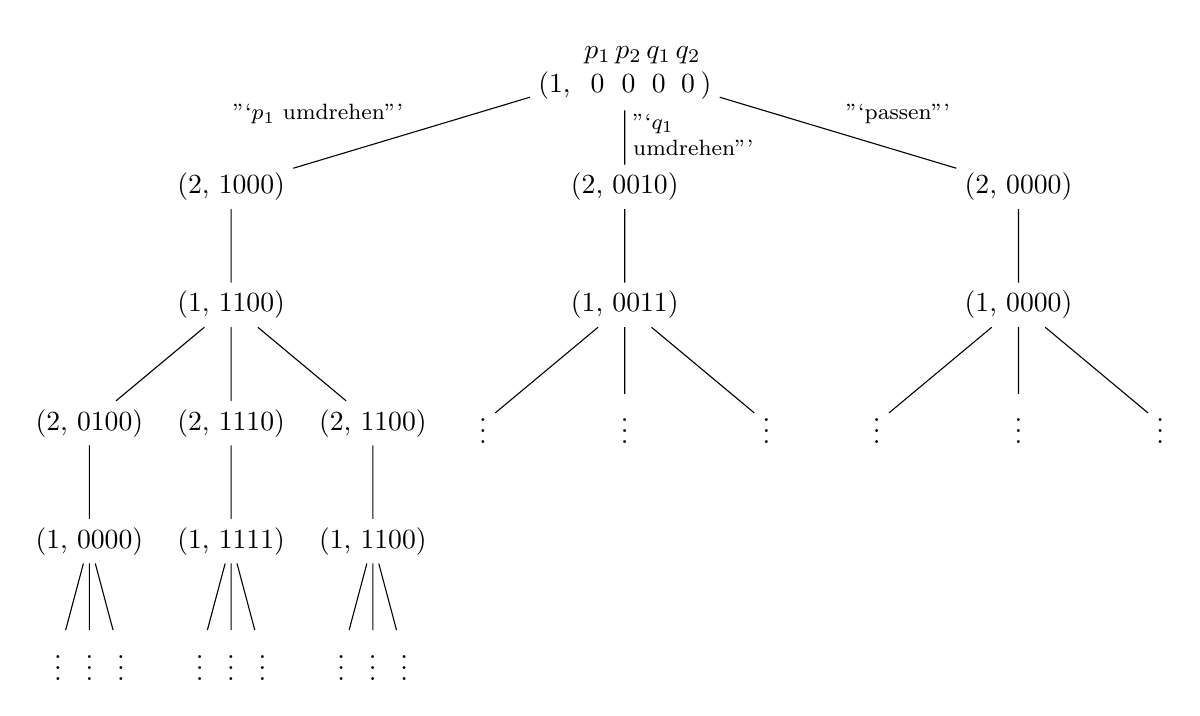
\begin{tikzpicture}[%
    every node/.style = {draw=none, fill=none, inner sep=1mm, minimum size=1mm},
    level 1/.style = {sibling distance = 50mm},
    level 2/.style = {sibling distance = 18mm},
    level 3/.style = {sibling distance = 18mm},
    level 4/.style = {sibling distance = 4mm},
    level 5/.style = {sibling distance = 4mm},
    edge from parent/.style = {draw=black, thin, -}%
  ]
    \node {(1,\, \begin{tabular}[b]{@{}c@{\,}c@{\,}c@{\,}c@{}}$p_1$&$p_2$&$q_1$&$q_2$\\0&0&0&0\end{tabular})}
      child {
        node {(2, 1000)}
        child {
          node {(1, 1100)}
          child {
            node {(2, 0100)}
            child {
              node {(1, 0000)}
              child {node {$\vdots$}}
              child {node {$\vdots$}}
              child {node {$\vdots$}}
            }
          }
          child {
            node {(2, 1110)}
            child {
              node {(1, 1111)}
              child {node {$\vdots$}}
              child {node {$\vdots$}}
              child {node {$\vdots$}}
            }
          }
          child {
            node {(2, 1100)}
            child {
              node {(1, 1100)}
              child {node {$\vdots$}}
              child {node {$\vdots$}}
              child {node {$\vdots$}}
            }
          }
        }
        edge from parent node[above left, draw=none, fill=none] {{\footnotesize "`$p_1$ umdrehen"'}}
      }
      child {
        node {(2, 0010)}
        child {
          node {(1, 0011)}
          child {node {$\vdots$}}
          child {node {$\vdots$}}
          child {node {$\vdots$}}
        }
%        edge from parent node[left=-1mm, draw=none, fill=none] {{\footnotesize \begin{tabular}{@{}rr@{}}"`$q_1$\\umdrehen"'\end{tabular}}}
        edge from parent node[right=0mm, draw=none, fill=none] {{\footnotesize \begin{tabular}{@{}ll@{}}"`$q_1$\\umdrehen"'\end{tabular}}}
      }
      child {
        node {(2, 0000)}
        child {
          node {(1, 0000)}
          child {node {$\vdots$}}
          child {node {$\vdots$}}
          child {node {$\vdots$}}
        }
        edge from parent node[above right, draw=none, fill=none] {{\footnotesize "`passen"'}}
      }
    ;
      
  \end{tikzpicture}%
\end{center}
%
Dabei zeigen die Kantenbeschriftungen in der 1.\ Ebene die Art des Zuges von Spielerin~2 an; die übrigen Beschriftungen kann man bei Bedarf leicht selbst ergänzen.

\par\vspace*{-.2\baselineskip}
Die Einträge \,$\vdots$\, bedeuten, dass der Baum ab dem entsprechenden Knoten
unendlich fortgesetzt wird.
Die Konfigurationen dieser Knoten kommen bis auf eine Ausnahme im bereits gezeichneten Baum vor; also ist deren Fortsetzung eindeutig bestimmt.
Die Ausnahme ist die Konfiguration $(1,1111)$;
dort kann man aber leicht selbst den Baum fortsetzen,
bis man in wenigen Schritten in allen Pfaden Positionen erreicht,
die bereits im gezeichneten Baum vorkommen.

\parII
\textsfbf{In Spiel (b)} hat Spielerin~2 \emph{keine} Gewinnstrategie,
denn wir haben im vorigen Beispiel bereits gesehen,
dass Spielerin~1 gewinnen kann.
Dazu muss man allerdings auch alle Spielverläufe betrachten,
die sich ergeben, wenn Spielerin~2 anstelle des mit $(*)$ markierten Zuges
die verbleibenden zwei möglichen Züge macht (vervollständige selbst!).

\pagebreak
% ===================================================================
\section*{T5.6~ Verbleibender Beweis der Korrektheit, {\boldmath "`$\Rightarrow$"'}}

\textsfbf{Behauptung.}~ $\Imc$ ist ein Modell von $W$ und $\Tmc_S$\,.

\parII
\textsfbf{Beweis.}~
Wegen $W^\Imc = \{w\}$ ist $W^\Imc \neq \emptyset$, und es bleibt zu zeigen,
dass \Imc jede der Konzeptinklusionen (1)--(8) erfüllt.
Wir zeigen hier, dass (2) erfüllt wird; die Argumentation für die übrigen Fälle
kann man leicht selbst ergänzen (probiere es aus!).

Um zu zeigen, dass
\[
  S_1 ~\sqsubseteq~ \exists r . (\neg V_0 \sqcap \cdots \sqcap \neg V_{n-1}) ~\sqcap~ \bigsqcap_{i < k} \exists r . V_i
  \tag{2}
\]
von \Imc erfüllt wird, betrachten wir eine beliebige Instanz von $S_1$,
d.\,h.\ ein Element $v \in S_1^\Imc$. Wir müssen zeigen, dass $v$ auch
eine Instanz der rechten Seite von (2) ist.

Da $\Delta^\Imc = V$ nach Definition von \Imc,
muss $v$ ein Knoten des Baums $B := (V,E,\ell)$ sein,
der die Gewinnstrategie repräsentiert.
Sei $\ell(v) = (i,\pi)$.
Nach Definition von $S_1^\Imc$ (Folie~5.29) ist $i=1$.
Da $B$ die Eigenschaft (c) von Gewinnstrategien erfüllt (Folie~5.23),
gibt es Knoten $v_0,\dots,v_k \in V$ mit $(v,v_i) \in E$ und $\ell(v_i) = (2,\pi_i)$
für alle $i \leq k$, so dass $\pi_0,\dots,\pi_k$ alle 1-Variationen von $\pi$ sind.
Nach Definition von $r^\Imc$ (Folie~5.29) folgt nun $(v,v_i) \in r^\Imc$ für alle  $i \leq k$,
und nach Definition von $V_j^\Imc$ gibt es
%
\begin{itemize}
  \item
    $u_i \in \{v_0,\dots,v_k\}$ mit $u_i \in V_i^\Imc$, für alle $i \leq k$,\quad und ein
  \item
    $u \in \{v_0,\dots,v_k\}$ mit $u \notin V_0^\Imc \cup \dots \cup V_{n-1}^\Imc$.
\end{itemize}
%
Also ist $v$ eine Instanz der rechten Seite von (2).
\qedhere

% ===================================================================
\section*{T5.7~ Verbleibender Beweis der Korrektheit, {\boldmath "`$\Leftarrow$"'}}

\textsfbf{Behauptung.}~ $(V,E,\ell)$ ist eine Gewinnstrategie für Spielerin~2.

\parII
\textsfbf{Beweis.}~
Wir zeigen, dass $(V,E,\ell)$ die vier Eigenschaften einer Gewinnstrategie (Folie~5.23) 
erfüllt. Dazu verwenden wir die Definition von $(V,E,\ell)$ von Folie~5.30
sowie die Tatsache, dass das zugrunde liegende Modell \Imc
die Konzeptinklusionen (1)--(8) erfüllt (Folien 5.27--5.28).
%
\begin{enumerate}
  \item[\textsfbf{(a)}]
    wird wegen (1) und der Definition von $(V,E,\ell)$ erfüllt.
  \item[\textsfbf{(b)}]
    Sei $\ell(v) = (2,\pi)$.
    Dann ist $v \in S_2^\Imc$.
    Wegen~(3) gibt es ein Element $v' \in \Delta^\Imc$
    mit $(v,v') \in r^\Imc$
    sowie 
    %
    \begin{enumerate}
      \item[(i)] 
        $v' \in (\lnot V_0 \sqcap \dots \sqcap \lnot V_{n-1})^\Imc$\quad oder
      \item[(ii)] 
        $v' \in V_i^\Imc$ für ein $i \in \{k,\dots,n-1\}$.
    \end{enumerate}
    %
    Im Fall~(ii) garantiert (4), dass $v' \notin V_j^\Imc$ für alle $j \neq i$.
    
    Sei nun $\ell(v') = (i',\pi')$.
    Wegen~(5) und~(6) ist somit in beiden Fällen $\pi'$ eine 2-Variation von $\pi$.
    Außerdem liefert~(7), dass $v' \in S_1^\Imc$, also $i'=1$.
  \item[\textsfbf{(c)}]
    lässt sich ähnlich wie (b) zeigen, indem man (2) statt (3) nutzt.
  \item[\textsfbf{(d)}]
    gilt wegen (8).
\qedhere
\end{enumerate}

\section*{{\boldmath T5.8~ Beispiel $i$-Typen und \ALC-Worlds}}

Sei $C_0=A\sqcap \exists r.B\sqcap\exists r.\neg B\sqcap\forall
r.\exists r.\neg A$. Dann ist $\textsf{rd}(C_0)=2$ und die Menge der Subkonzepte: 
%
\[\textsf{sub}(C_0)=\{C_0,A,\exists r.B,B,\exists r.\neg B,\neg B,\forall
r.\exists r.\neg A,\exists r.\neg A,\neg A\}.\]
%
Beispiele für $i$-Typen, $i\leq 2$: 
%
\begin{align*}
  %
  \text{$0$-Typ:} \quad & \{A,\neg B\} \\
  %
  \text{$1$-Typ:} \quad & \{A, B,\exists r.B,\exists r.\neg B\} \\
  %
  \text{$2$-Typ:} \quad & \{\neg A,\neg B,\exists r.B,\forall r.\exists
  r.\neg A\}
  %
\end{align*}

\ALC-Worlds$(C_0)$ hat einen erfolgreichen Lauf: 

Zunächst wird der initiale Typ $t_0=\{C_0,A,\exists r.B,\exists r.\neg
B,\forall r.\exists r.\neg A,\neg B\}$ geraten und folgender Aufruf zu
$\texttt{recurse}$ getätigt: 
%
\[\texttt{recurse}(t_0,2,C_0)\]
%
Der Lauf kann nun als \emph{Aufrufbaum} dargestellt werden, wobei die Kanten
immer mit der ``verursachenden'' Existenzrestriktion und dem
entsprechenden $S$ beschriftet sind: 
%
\begin{center}
  \begin{tikzpicture}[%
    >=Latex,baseline=.2pt,
    every edge/.style={draw=black,thin},
    every node/.style = {draw=none, fill=none, inner sep=1mm, minimum size=1mm},
    level 1/.style = {sibling distance = 80mm, level distance=18mm},
    level 2/.style = {sibling distance = 18mm, level distance=20mm},
    level 3/.style = {sibling distance = 18mm},
    level 4/.style = {sibling distance =  4mm},
    level 5/.style = {sibling distance =  4mm},
    edge from parent/.style = {draw=black, thin, ->}%
  ]
  \node {$\texttt{recurse}(t_0,2,C_0)$}
      child {
	node {$\texttt{recurse}(\{B,\exists r.\neg A,A\},1,C_0)$}
        child {
	  node {$\texttt{recurse}(\{\neg A,\neg B\},0,C_0\})$}
	  edge from parent node[right, draw=none, fill=none]
	{{\footnotesize\begin{tabular}{@{}ll@{}}$\exists r.\neg
	  A$\\$S=\{\neg A\}$\end{tabular}}}
        }
        edge from parent node[above left=-1mm and -1mm, draw=none, fill=none]
	{\footnotesize\begin{tabular}{@{}ll@{}}$\exists r.B$\\$S=\{B,\exists r.\neg
	  A\}$\end{tabular}}
      }
      child {
	node {$\texttt{recurse}(\{\neg B,\exists r.\neg A,A\},1,C_0)$}
        child {
          node {$\texttt{recurse}(\{\neg A,B\},0,C_0)$}
	  edge from parent node[right, draw=none, fill=none]
	{{\footnotesize\begin{tabular}{@{}ll@{}}$\exists
	  r.\neg A$\\$S=\{\neg A\}$\end{tabular}}}
        }
        edge from parent node[above right=-1mm and -1mm, draw=none, fill=none]
	{{\footnotesize\begin{tabular}{@{}ll@{}}$\exists r.\neg
	  B$\\$S=\{\neg B,\exists r.\neg
	  A\}$\end{tabular}}}
      }
    ;
      
  \end{tikzpicture}%
\end{center}

Aus dem Aufrufbaum von \texttt{recurse} können wir nun das folgende
Modell ablesen:
%
\begin{center}
  \begin{tikzpicture}[%
    >=Latex,baseline=.2pt,
    every node/.style={circle,draw=black,thin,fill=black!10,inner sep=.4mm,minimum size=5mm},
%    every node/.style = {draw, fill, circle, inner sep=1mm, minimum size=1mm},
    every edge/.style={draw=black,thin},
    level 1/.style = {sibling distance = 80mm},
    level 2/.style = {sibling distance = 18mm},
    level 3/.style = {sibling distance = 18mm},
    level 4/.style = {sibling distance = 4mm},
    level 5/.style = {sibling distance = 4mm},
    edge from parent/.style = {draw=black, thin, ->}%
  ]
  \node[label=above right:{$A$}] {}
      child {
	node[label=left:{$A,B$} ] {}
        child {
	  node {}
	  edge from parent node[right, draw=none, fill=none]
	{$r$}
        }
        edge from parent node[above left, draw=none, fill=none]
	{$r$}
      }
      child {
	node[label=right:{$A$}] {}
        child {
          node [label=right:{$B$}]{}
	  edge from parent node[right, draw=none, fill=none]
	{$r$}
        }
        edge from parent node[above right, draw=none, fill=none]
	{$r$}
      }
    ;
      
  \end{tikzpicture}%
\end{center}

\goodbreak
% ===================================================================
\section*{T5.9~ Beispiel eines \textsf{PSpace}-Spiels}

Wir betrachten folgendes Beispiel.

\begin{itemize}
  \item
    $\varphi = (\lnot p_1 \to p_2) \land (\lnot p_2 \to (p_4 \to \lnot p_3))$
  \item
    Spielerin 1 kontrolliert Variablen $p_1,p_3$;
    Spielerin 2 kontrolliert Variablen $p_2,p_4$;
    die Variablen werden genau in der Reihenfolge $p_1,\dots,p_4$ gespielt.
  \item
    (Eine Anfangsbelegung gibt es nicht.)
\end{itemize}
%
Jeder Spielverlauf besteht somit aus genau 4 Zügen.
Ein möglicher Spielverlauf, bei dem beide Spielerinnen "`optimal"' spielen,
ist folgender:
%
\begin{itemize}
  \item
    Spielerin~1 belegt $p_1$ mit 1.
    \par
    Sonst würde Spielerin~2 gewinnen, indem sie $p_2$ mit 0 belegt,
    wodurch die erste Implikation und damit die gesamte Formel nicht erfüllt ist.
  \item
    Spielerin~2 belegt $p_2$ mit 0.
    \par
    Sonst wäre die zweite Implikation immer wahr, und Spielerin~1 würde gewinnen.
  \item
    Spielerin~1 belegt $p_3$ mit 0.
    \par
    Damit wird die dritte Implikation wahr und somit auch die zweite, egal wie $p_4$ belegt wird.
  \item
    Spielerin~2 belegt $p_4$ mit 0.
\end{itemize}
%
Die gespielte Belegung 1000 erfüllt $\varphi$; somit gewinnt Spielerin~1.

% ===================================================================
\section*{T5.10~ Beispiel für eine Gewinnstrategie}

Aus den Überlegungen im vorangegangenen Beispiel ergibt sich folgende Gewinnstrategie
für Spielerin~1.
%
\begin{center}
  \begin{tikzpicture}[%
    >=Latex,baseline=.2pt,
    every edge/.style={draw=black,thin},
    level 1/.style = {sibling distance = 40mm, level distance = 10mm},
    level 2/.style = {sibling distance = 40mm, level distance = 11mm},
    level 3/.style = {sibling distance = 16mm, level distance = 12mm},
    level 4/.style = {sibling distance = 16mm, level distance = 12mm},
    edge from parent/.style = {draw=black, thin, -}%
  ]
    \node {$\varepsilon$}
      child {
        node {1}
        child {
          node (10) {10}
          child {
            node (100) {100}
            child {
              node {1000}
            }
            child {
              node {1001}
            }
          }
        }
        child {
          node (11) {11}
          child {
            node (111) {111}
            child {
              node {1110}
            }
            child {
              node {1111}
            }
          }
        }
      }
    ;
    
    \node[above left =0mm and 8mm of 10]  (10l)  {};
    \node[above left =0mm and 8mm of 100] (100l) {};
    \node[above right=0mm and 8mm of 11]  (11l)  {};
    \node[above right=0mm and 8mm of 111] (111l) {};
    
    \path[->]
      (10l)  edge (10)
      (100l) edge (100)
      (11l)  edge (11)
      (111l) edge (111)
    ;
    
    \node [left =-2mm of 10l]  {\footnotesize 2.\ Implikation "`aktiviert"'};
    \node [left =-2mm of 100l] {\footnotesize 2.\ Implikation wahr};
    \node [right=-2mm of 11l]  {\footnotesize 2.\ Implikation "`deaktiviert"'};
    \node [right=-2mm of 111l] {\footnotesize \begin{tabular}{@{}l@{}}Hier ist es egal,\\was Spielerin 1 tut.\end{tabular}};
      
  \end{tikzpicture}%
\end{center}
%
Dabei sind die (partiellen) Belegungen gemäß Definition~5.22 als Wörter notiert;
in der Wurzel (leeres Wort~$\varepsilon$) ist also noch keine Variable gesetzt,
im Kind 1 wurde $p_1$ auf 1 gesetzt usw.
In jedem Blatt steht eine Belegung, die $\varphi$ erfüllt.


\section*{T5.11~ Beispiele für Rollenwertvergleiche}

\begin{enumerate}

  \item \emph{globaler Rollenwertvergleich:} wie auf Folie 5.64 unten
    %
    \[\text{hört}\circ\text{angebotenVon}\sqsubseteq
    \text{eingeschriebenAn}\]
    %
    Umgangssprachlich: ``wer einen Kurs hört, der irgendwo angeboten
    wird, ist ebenda eingeschrieben''

  \item \emph{lokaler Rollenwertvergleich:}
    %
    \[\text{KorrekterStudent}\equiv \text{Student}\sqcap
    (\text{hört}\circ\text{angebotenVon}\sqsubseteq
  \text{eingeschriebenAn})\]
    %
    Umgangssprachlich: ``korrekte Studierende sind Studierende, die an
    allen Einrichtungen, an denen sie einen Kurs hören, auch
    eingeschrieben sind''
    
\end{enumerate}

Betrachten wir die folgende Interpretation $\mathcal{I}$:

\begin{center}
  \begin{tikzpicture}[%
    >=Latex,baseline=.2pt,
    every node/.style={ellipse,draw,fill=none,inner sep=.4mm,minimum size=1mm},
    every edge/.style={draw=black,thin}
  ]
  \node (p1)  [label=above:{$\text{Student}$}] {$\text{hanna}$}; 
  \node (p2)  [below=2cm of p1]  {$\text{uni$\_$hb}$};
  \node (p3)  [below right=1cm of p1]  {$\text{BL}$};
    
  \node (q1)  [right=4cm of p1, label=above:{$\text{Student}$}] {$\text{klaus}$};
  \node (q2)  [below=2cm of q1]  {$\text{hs$\_$hb}$};
  \node (q3)  [below right=1cm of q1]  {$\text{fahrzeugbau}$};
   
  \draw[->] (p1) edge node[draw=none,left=-6mm] {$\text{eingeschriebenAn}$} (p2);
  \draw[->] (p1) edge node[draw=none,pos=.2, right=1mm] {$\text{hört}$} (p3);
  \draw[->] (p3) edge node[draw=none,pos=.6,right=-3mm]
  {$\text{angebotenVon}$} (p2);

  \draw[->] (q1) edge node[draw=none,left=-6mm] {$\text{eingeschriebenAn}$} (q2);
  \draw[->] (q1) edge node[draw=none,pos=.2,right=2mm] {$\text{hört}$} (q3);
  \draw[->] (q3) edge node[draw=none,pos=.6,right=-3mm]
  {$\text{angebotenVon}$} (q2);

  \draw[->] (q1) edge node[draw=none,above=1mm] {$\text{hört}$} (p3);

%     \path[->]
%       (1p1) edge[out=200,in=160,looseness=2.7] node [pos=.55,left=1mm] {{\footnotesize 1}} (2p1)
%       (2p1) edge[out=200,in=160,looseness=2.7] node (s1) [pos=.55,left=1mm] {{\footnotesize 2}} (3p1)
%       (3p1) edge[out=200,in=160,looseness=2.7] node [pos=.55,left=1mm] {{\footnotesize 1}} (4p1)
%       (53) edge[out=350,in=10,looseness=2.7] node (s2) [pos=.55,right=1mm] {{\footnotesize 1}} (63)
%       
%       (4all) edge node [pos=.4,left=2mm]  {{\footnotesize 2}} (51)
%       (4all) edge node [pos=.4,left=0mm]  {{\footnotesize 2}} (52)
%       (4all) edge node [pos=.4,right=2mm] {{\footnotesize 2}} (53)
%       
%     ;
    
  \end{tikzpicture}
\end{center}

Dann gilt: 

\begin{align*}
  %
  (\text{hört}\ \text{angebotenVon})^\Imc(\text{hanna}) &=
  \{\text{uni$\_$hb}\} \\
  %
  (\text{hört}\ \text{angebotenVon})^\Imc(\text{klaus}) &=
  \{\text{uni$\_$hb},\text{hs$\_$hb}\} \\
  %
  (\text{hört}\ \text{angebotenVon})^\Imc(\text{BL}) &= \emptyset \\
  %
  & ~\vdots \\
  %
  (\text{eingeschriebenAn})^\Imc(\text{hanna}) &=
  \{\text{uni$\_$hb}\} \\
  %
  (\text{eingeschriebenAn})^\Imc(\text{klaus}) &=
  \{\text{hs$\_$hb}\} \\
  %
  (\text{eingeschriebenAn})^\Imc(\text{BL}) &= \emptyset
  \\
  %
  & ~\vdots
  %
\end{align*}
%
Und damit:
%
\[{\underbrace{(\text{hört}\circ\text{angebotenVon}\sqsubseteq
  \text{eingeschriebenAn})}_{\rho}}^\Imc =
\{\text{hanna},\text{BL},\text{fahrzeugbau},\text{uni$\_$hb},\text{hs$\_$hb}\}\]
Deshalb gilt:
%
\begin{itemize}

  \item $\text{hanna}\in \text{KorrekterStudent}^\Imc$, aber
    $\text{klaus}\notin \text{KorrekterStudent}^\Imc$;

  \item $\Imc$ erfüllt $\rho$ \emph{nicht};


\end{itemize}


\section*{T5.12~ Formalisierung von Dominoproblemen}

Die Instanz des Dominoproblems ist $\mathcal{D} = (T,H,V)$: 
%
\begin{align*}
  %
  T & =\{t_1,t_2,t_3\} \\
  %
  H & = \{(t_1,t_2), (t_2,t_1), (t_3,t_3) \} \\
  %
  V & = \{(t_1,t_3), (t_2,t_3), (t_3,t_1), (t_3,t_2) \}
  %
\end{align*}
%
Beachtet: die Quadrate dürfen \emph{nicht gedreht} werden. 

Die angegebene Lösung (Folie 5.69) ist dann: 
%
\begin{align*}
  %
  &\tau(0,0) = t_1, \quad\tau(1,0)=t_2, \quad\tau(2,0)=t_1,\ldots, \\
  %
  &\tau(0,1) = t_3, \quad\tau(1,1)=t_3, \quad\ldots, \\
  %
  &\tau(0,2) = t_1, \quad\ldots, \\
  %
  & \vdots
  %
\end{align*}


\section*{T5.13~ $\Rightarrow$-Richtung von Lemma~5.33}

Die konstruierte Interpretation sieht wie folgt aus (die Konzeptnamen
$A_{t_i}$ sind zufällig gewählt):

\begin{center}
  \begin{tikzpicture}[%
    >=Latex,baseline=.2pt,
    every node/.style={circle,draw,fill=none,inner sep=.4mm,minimum size=1mm},
    every edge/.style={draw=black,thin}
  ]
  \node (p1)  [label=below right:{$A_{t_1}$}] {$\langle 0,0\rangle$}; 
  \node (p2)  [label=below right:{$A_{t_2}$},right=2cm of p1]
  {$\langle 1,0\rangle$};
  \node (p3)  [label=below right:{$A_{t_3}$},right=2cm of p2]
  {$\langle 2,0\rangle$};
  \node (p4)  [draw=none,right=2cm of p3]  {$\ldots$};
    
  \node (q1)  [label=below right:{$A_{t_3}$},above=2cm of p1]
  {$\langle 0,1\rangle$}; 
  \node (q2)  [label=below right:{$A_{t_1}$},right=2cm of q1]
  {$\langle 1,1\rangle$};
  \node (q3)  [label=below right:{$A_{t_2}$},right=2cm of q2]
  {$\langle 2,1\rangle$};
  \node (q4)  [draw=none,right=2cm of q3]  {$\ldots$};

  \node (r1)  [draw=none, above=2cm of q1] {$\vdots$}; 
  \node (r2)  [draw=none, above=2cm of q2]  {$\vdots$};
  \node (r3)  [draw=none, above=2cm of q3]  {$\vdots$};
    
%   \path[->] (p1) edge (p2) edge (p3) edge (p4);
  \draw[->] (p1) edge node[above,draw=none] {$r_x$} (p2);
  \draw[->] (p2) edge node[above,draw=none] {$r_x$} (p3);
  \draw[->] (p3) edge node[above,draw=none] {$r_x$} (p4);

  \draw[->] (q1) edge node[above,draw=none] {$r_x$} (q2);
  \draw[->] (q2) edge node[above,draw=none] {$r_x$} (q3);
  \draw[->] (q3) edge node[above,draw=none] {$r_x$} (q4);

  \draw[->] (p1) edge node[right,draw=none] {$r_y$} (q1);
  \draw[->] (q1) edge node[right,draw=none] {$r_y$} (r1);

  \draw[->] (p2) edge node[right,draw=none] {$r_y$} (q2);
  \draw[->] (q2) edge node[right,draw=none] {$r_y$} (r2);

  \draw[->] (p3) edge node[right,draw=none] {$r_y$} (q3);
  \draw[->] (q3) edge node[right,draw=none] {$r_y$} (r3);

  \end{tikzpicture}
  %
\end{center}

Man kann relativ leicht zeigen, dass die konstruierte Interpretation
alle Konzeptinklusionen der TBox $\Tmc_{\mathcal{D}}$ erfüllt
(siehe Fragebogen).



\section*{T5.14~ $\Leftarrow$-Richtung von Lemma~5.33 -- Vorbereitung}

Sei $\Imc$ ein Modell von $\top$ bzgl. \Tmc.
Wir konstruieren in zwei Schritten die Abbildung
$f:\mathbb{N}\times\mathbb{N}\to \Delta^\Imc$.

\smallskip
\textbf{Schritt 1:}

\begin{itemize}

  \item Setze $f(0,0)=d$ für ein beliebiges $d\in \Delta^\Imc$.

  \item Für alle $i=0,1,2,\ldots$:

    \begin{itemize}

      \item wähle $d\in \Delta^\Imc$ mit $(f(i,i),d)\in r_x^\Imc$ und
	setze $f(i+1,i)=d$

      \item wähle $e\in \Delta^\Imc$ mit $(f(i+1,i),e)\in r_y^\Imc$ und
	setze $f(i+1,i+1)=e$

    \end{itemize}

    Beachte: Alle diese Elemente $d,e$ existieren, da \Imc die
    Konzeptinklusion~(1)
    %
    \[\top\sqsubseteq \exists r_x.\top\sqcap \exists
    r_y.\top\] 
    %
    erfüllt.

\end{itemize}

\smallskip
\textbf{Schritt 2:} Wir ``vervollständigen'' $f$ indem wir die
folgenden Schritte erschöpfend anwenden: 
%
\begin{itemize}

  \item Wenn $f(i,j)$, $f(i+1,j)$ und $f(i+1,j+1)$ definiert sind und
    $f(i,j+1)$ noch nicht, dann wähle $d\in \Delta^\Imc$ mit
    $(f(i,j),d)\in r_y^\Imc$ und $(d,f(i+1,j+1))\in r_x^\Imc$ und
    setze $f(i,j+1)=d$.

  \item Wenn $f(i,j)$, $f(i,j+1)$ und $f(i+1,j+1)$ definiert sind und
    $f(i+1,j)$ noch nicht, dann wähle $d\in \Delta^\Imc$ mit
    $(f(i,j),d)\in r_x^\Imc$ und $(d,f(i+1,j+1))\in r_y^\Imc$ und
    setze $f(i+1,j)=d$.

\end{itemize}
%
Alle diese Elemente $d$ existieren da $\Imc$ die
Rollenwertvergleiche~(4) und die Konzeptinklusion~(1) erfüllt. 



\section*{T5.15~ $\Leftarrow$-Richtung von Lemma~5.33}

Wir zeigen, dass $\tau$ eine Lösung ist: 
%
\begin{itemize}

  \item \emph{$\tau$ ist wohldefiniert}: Wegen
    Konzeptinklusion~(2) gibt es für jedes $d\in \Delta^\Imc$ genau
    ein $t$ sodass $d\in A_t^\Imc$. Damit gibt 
    es für jedes $(i,j)\in \mathbb{N}\times\mathbb{N}$ genau ein $t$
    mit $\tau(i,j)=t$.

  \item \emph{$\tau$ ist eine Lösung}: Wegen
    Konzeptinklusionen~(3) sind die horizontalen bzw.\ vertikalen
    Passbedingungen erfüllt. 

\end{itemize}


\bigskip\bigskip
\textbf{Dokument wird fortgesetzt.}

\parIII
\parIII
%
% ===================================================================
% ===================================================================
% ===================================================================
\part{Effiziente Beschreibungslogiken}

% ===================================================================
\section*{T6.1~ Beispiele Simulation}

\textsf{\textbf{Beispiel 1}}\qquad
%
\begin{tikzpicture}[%
  >=Latex,baseline=11pt,
  every state/.style={draw=black,thin,fill=black!10,inner sep=.6mm,minimum size=6mm},
  every edge/.style={draw=black,thin}
]
  \node[state] (leps)                                    {};
  \node[state] (l0)   [below      =8mm          of leps] {};
  \node[state] (l00)  [below left =8mm and  7mm of l0]   {};
  \node[state] (l01)  [below right=8mm and  7mm of l0]   {};
  
  \node[state] (reps) [right=50mm of leps]             {};
  \node[state] (r0)  [below left =8mm and 7mm of reps] {};
  \node[state] (r1)  [below right=8mm and 7mm of reps] {};
  \node[state] (r00) [below      =8mm         of r0]   {};
  
  \node [left=0mm of leps] {$A$};
  \node [left=0mm of l00]  {$A$};
  \node [left=0mm of l01]  {$B$};
  
  \node [right=0mm of reps] {$A$};
  \node [right=0mm of r1]   {$A,B$};
  \node [right=0mm of r00]  {$A,B,C$};

  \node [above left=0mm and 10mm of leps] {$\Imc_1$};
  \node [above left=0mm and 10mm of reps] {$\Imc_2$};

  \path[->]
    (leps) edge node[pos=.6, left]       {$r$} (l0)
    (l0)   edge node[pos=.4, left =.5mm] {$r$} (l00)
    (l0)   edge node[pos=.4, right=.5mm] {$r$} (l01)

    (reps) edge node[pos=.4,left =1mm] {$r$} (r0)
    (reps) edge node[pos=.3,right=1mm] {$s$} (r1)
    (r0)   edge node[left]             {$r$} (r00)
  ;
  
  \path[->,densely dashed]
    (leps) edge [bend right=10] node [pos=.45,above] {$\rho$} (reps)
    (l0)   edge [bend right=10] node [pos=.60,above] {$\rho$} (r0)
    (l01)  edge [bend right=10] node [pos=.42,above] {$\rho$} (r00)
    (l00)  edge [bend right=20] node [pos=.70,below] {$\rho$} (r00)
  ;
\end{tikzpicture}
%
\parIII\parI
\textsf{\textbf{Beispiel 2}}\qquad
%
\begin{tikzpicture}[%
  >=Latex,baseline=11pt,
  every state/.style={draw=black,thin,fill=black!10,inner sep=.6mm,minimum size=6mm},
  every edge/.style={draw=black,thin}
]
  \node[state] (d2)                                  {};
  \node[state] (d3) [below left =7mm and  8mm of d2] {};
  \node[state] (d5) [below right=7mm and  8mm of d2] {};
  \node[state] (d4) [below right=7mm and  8mm of d3] {};
  
  \node[state] (d1) [right=45mm of d2] {$e$};
  
  \node [left=0mm of d2] {$A$};
  \node [left=0mm of d3] {$A,B$};
  \node [left=0mm of d4] {$B$};
  
  \node [right=0mm of d1] {$A,B$};

  \node [above left=0mm and 10mm of d2] {$\Imc_1$};
  \node [above left=0mm and 10mm of d1] {$\Imc_2$};

  \path[->]
    (d2) edge             node[pos=.4,left =1mm] {$r$} (d3)
    (d3) edge             node[pos=.6,left =1mm] {$s$} (d4)
    (d4) edge             node[pos=.3,right=1mm] {$r$} (d5)
    (d5) edge             node[pos=.6,right=1mm] {$s$} (d2)
    
    (d1) edge[loop below] node[below]            {$r,s$} ()
  ;
  
  \path[->,densely dashed]
    (d2) edge [bend left = 3]   node [pos=.47,above] {$\rho$} (d1)
    (d3) edge [bend right= 1.5] node [pos=.60,above] {$\rho$} (d1)
    (d5) edge [bend right= 9]   node [pos=.25,below] {$\rho$} (d1)
    (d4) edge [bend right=18]   node [pos=.42,below] {$\rho$} (d1)
  ;
\end{tikzpicture}%
%
\parIII
Wenn nur die Konzept- und Rollennamen $A,B,r,s$ verwendet werden,
gilt mit $\Imc_2$ aus Beispiel 2 sogar für \emph{jede} Interpretation \Imc
und \emph{jedes} Element $d \in \Delta^\Imc$:
\[
  (\Imc,d) \precsim (\Imc_2,e)
\]

% ===================================================================
\section*{T6.2~ Beweis des Simulationstheorems}

\textsfbf{Theorem 6.3}~
Seien $\Imc_1,\Imc_2$ Interpretationen, $d_1 \in \Delta^{\Imc_1}$ und $d_2 \in \Delta^{\Imc_2}$.

\par\smallskip
Wenn $(\Imc_1,d_1) \precsim (\Imc_2,d_2)$,~ dann gilt f\"ur alle \EL-Konzepte $C$:
\[
  d_1 \in C^{\Imc_1}\qquad\text{impliziert}\qquad d_2 \in C^{\Imc_2}
\]      

\par\noindent
\begin{beweis}
  Sei $\rho$ eine Simulation von $\Imc_1$ nach $\Imc_2$ mit $d_1\mathrel{\rho} d_2$.
  Wir beweisen die Behauptung per Induktion über die Struktur von $C$.
  Der Beweis ist letztlich derselbe wie für die entsprechenden Fälle
  des Bisimulationstheorems (Theorem~3.2).
  %
  \begin{description}
    \item[Induktionsanfang.]
      Wenn $C=A$ für einen Konzeptnamen $A$,
      dann gilt 
      nach Bedingung (1) für Simulationen (Definition~6.2) wie gewünscht:
      $d_1 \in A^{\Imc_1}$ impliziert $d_2 \in A^{\Imc_2}$.
      
      Wenn $C=\top$, dann gilt die Implikation, weil die rechte Seite trivialerweise wahr ist.
    \item[Induktionsschritt.]
      Wir müssen nur noch zwei Fälle gemäß des äußersten Konstruktors
      von $C$ unterscheiden $(\sqcap,\exists)$:
      %
      \begin{description}
        \item[{\boldmath $C=D \sqcap E$.}]
          Wir können genauso wie im entsprechenden Fall des Beweises des Bisimulationstheorems
          mittels Semantik von "`$\sqcap$"' und Induktionsvoraussetzung argumentieren:
          ~ %Dann gilt:
          %
          \parI
          \begin{center}
            \begin{tabular}{@{}llp{40mm}l@{}}
              $d_1 \in C^{\Imc_1}$
              & $\Rightarrow$ & $d_1 \in D^{\Imc_1}$ und $d_1 \in E^{\Imc_1}$ & (Semantik "`$\sqcap$"') \\
              & $\Rightarrow$ & $d_2 \in D^{\Imc_2}$ und $d_2 \in E^{\Imc_2}$ & (Induktionsvoraussetzung)\\
              & $\Rightarrow$ & $d_2 \in C^{\Imc_2}$                          & (Semantik "`$\sqcap$"')
            \end{tabular}
          \end{center}
          \parI
        \item[{\boldmath $C=\exists r.D$.}]
          Hier können wir genauso wie im $\exists$-Fall des Beweises des Bisimulationstheorems
          (Richtung "`$\Rightarrow$"') mittels Semantik von "`$\exists$"', Bedingung (2) von Simulationen und Induktionsvoraussetzung argumentieren:
          %
          \parIII
          $d_1 \in C^{\Imc_1}$ \\
          %
          \begin{tabular}{@{}l@{}l@{~\,}l@{~~}l@{}}
            & $\Rightarrow$ & es gibt $e_1 \in \Delta^{\Imc_1}$ mit $(d_1,e_1) \in r^{\Imc_1}$ und $e_1 \in D^{\Imc_1}$ & (Semantik "`$\exists$"') \\
            & $\Rightarrow$ & es gibt $e_2 \in \Delta^{\Imc_2}$ mit $(d_2,e_2) \in r^{\Imc_2}$ und $e_1\rho e_2$ & (Bedingung~(2) Simul.) \\
            & $\Rightarrow$ & $e_2 \in D^{\Imc_2}$ & (Induktionsvorauss.) \\
            & $\Rightarrow$ & $d_2 \in (\exists r.D)^{\Imc_2}$ & (Semantik "`$\exists$"')
          \end{tabular}
          %
          \par\vspace*{-1.1\baselineskip}
          \qedhere
      \end{description}
  \end{description}
\end{beweis}

% ===================================================================
\section*{T6.3~ Simulation versus Bisimulation; Ausdrucksstärke.}

\newenvironment{tikzpicturetwointerp}{%
  \begin{tikzpicture}[%
    >=Latex,baseline=11pt,
    every state/.style={draw=black,thin,fill=black!10,inner sep=.6mm,minimum size=6mm},
    every edge/.style={draw=black,thin}
  ]
    \node[state] (leps)                                   {$d_1$};
    \node[state] (l0)   [below      =8mm         of leps] {};
    
    \node[state] (reps) [right=20mm of leps]              {$d_2$};
    \node[state] (r0)   [below left =9.5mm and 4mm of reps] {};
    \node[state] (r1)   [below right=9.5mm and 4mm of reps] {};
    
    \node [left=0mm of l0]  {$A$};
    
    \node [right=0mm of r0]   {$A$};
  
    \node [above left=0mm and 1mm of leps] {$\Imc_1$};
    \node [above left=0mm and 1mm of reps] {$\Imc_2$};
  
    \path[->]
      (leps) edge node[pos=.6, left]       {$r$} (l0)
  
      (reps) edge node[pos=.4,left =1mm] {$r$} (r0)
      (reps) edge node[pos=.4,right=1mm] {$r$} (r1)
    ;
}{%
  \end{tikzpicture}
}%

\textsfbf{Lemma 6.4.}
Es gibt $(\Imc_1,d_1)$ und $(\Imc_2,d_2)$, so dass:
%
\begin{enumerate}
  \item[(1)]
    $(\Imc_1,d_1) \precsim (\Imc_2,d_2)$ ~und~ $(\Imc_2,d_2) \precsim (\Imc_1,d_1)$
  \item[(2)]
    $(\Imc_1,d_1) \not\sim (\Imc_2,d_2)$
\end{enumerate}
%
\parII
\textsfbf{Beweis.}~
Wir wählen $(\Imc_1,d_1)$ und $(\Imc_2,d_2)$ wie folgt.
%
\begin{center}
  \begin{tikzpicturetwointerp}
  \end{tikzpicturetwointerp}    
\end{center}
%
Punkt~(1) aus dem Lemma wird durch folgende Simulationen $\rho_1,\rho_2$ bezeugt:
\begin{center}
%  \begin{tabular}{c@{\qquad}|@{\qquad}c}
    \begin{tikzpicturetwointerp}
      \path[->,densely dashed]
        (leps) edge [bend right= 5] node [pos=.30,above] {$\rho_1$} (reps)
        (l0)   edge [bend right=10] node [pos=.50,above] {$\rho_1$} (r0)
      ;
    \end{tikzpicturetwointerp}
%    &
    \hspace*{20mm}
    \begin{tikzpicturetwointerp}
      \path[<-,densely dashed]
        (leps) edge [bend right= 5] node [pos=.30,above] {$\rho_2$} (reps)
        (l0)   edge [bend right=10] node [pos=.50,above] {$\rho_2$} (r0)
        (l0)   edge [bend right=25] node [pos=.20,below] {$\rho_2$} (r1)
      ;
    \end{tikzpicturetwointerp}
%  \end{tabular}
\end{center}
%
Punkt~(2) gilt, denn wenn es eine Bisimulation gäbe,
dann müsste diese mindestens $\rho_1$ und $\rho_2$ enthalten,
aber die "`unterste Kante"' von $\rho_2$ verbindet zwei Elemente,
die nicht Instanzen derselben Konzeptnamen sind
(und verstößt damit gegen Bedingung 1 von Bisimulationen).
\qedhere

\goodbreak
\parIII
\textsfbf{Lemma 6.5.}
Das \ALC-Konzept $\forall r.A$ ist nicht in $\EL$ ausdrückbar.
%
\parII
\textsfbf{Beweis.}~
Angenommen es gebe ein \EL-Konzept $C$, das äquivalent zu $\forall r.A$ ist.
Da für die obige Interpretation $\Imc_1$ gilt $d_1 \in (\forall r.A)^{\Imc_1}$,
ist also $d_1 \in C^{\Imc_1}$.
Da $(\Imc_1,d_1) \precsim (\Imc_2,d_2)$, folgt mit dem Simulationstheorem
(Theorem~6.3) $d_2 \in C^{\Imc_2}$,
was im Widerspruch zu $d_2 \notin (\forall r.A)^{\Imc_2}$ steht.
\qedhere

Zwei Anmerkungen zu Lemma~6.5 und dessen Beweis:
%
\begin{itemize}
  \item 
    In \ELI{} -- der Erweiterung von \EL mit inversen Rollen --
    sind dagegen manche Werterestriktionen ausdrückbar;
    nämlich ist $A \sqsubseteq \forall r.B$ äquivalent zu $\exists r^-.A \sqsubseteq B$.
  \item
    Man kann aus dem Beweis des Lemmas wieder die Methodologie
    zum Beweisen der Nicht-Ausdrückbarkeit als ein separates Theorem
    herausarbeiten, analog zu Theorem~3.5.
\end{itemize}


% ===================================================================
\section*{T6.4~ {\boldmath Erfüllbarkeit in \EL}}

\textsfbf{Lemma 6.6.}
Jedes \EL-Konzept ist erfüllbar bzgl.\ jeder \EL-TBox.
%
\parII
\textsfbf{Beweis.}~
Betrachte die folgende Interpretation \Imc.
%
\begin{center}
  \begin{tikzpicture}[%
    >=Latex,baseline=11pt,
    every state/.style={draw=black,thin,fill=black!10,inner sep=.6mm,minimum size=6mm},
    every edge/.style={draw=black,thin}
  ]
    \node[state] (d) {$d$};
    
    \node [left=0mm of d] {$A_1,A_2,\dots$};
  
    \node [above left=1mm and 2mm of d] {$\Imc$};
  
    \path[->]
      (d) edge[loop right] node[right]            {$r_1,r_2,\dots$} ()
    ;    
  \end{tikzpicture}%
\end{center}
%
Dabei bedeutet die Schreibweise "`$\dots$"', dass $d$ eine Instanz \emph{jedes} Konzeptnamens
und $(d,d)$ eine Instanz \emph{jedes} Rollennamens ist.
Nun ist leicht zu sehen, das für jedes \EL-Konzept $C$ gilt: $C^\Imc = \{d\}$
(was man bequem per Induktion über die Struktur von $C$ zeigen kann).
Also ist \Imc ein Modell jedes \EL-Konzeptes
und damit auch jeder \EL-TBox.
\qedhere

% ===================================================================
\section*{T6.5~ Kanonisches Modell ist ein Modell}

\textsfbf{Lemma 6.8.}
F\"ur alle \EL-Konzepte $C$ gilt:~
Die Interpretation $\Imc_C$ ist Modell von $C$ mit 
$d_W \in C^{\Imc_C}$.
%
\parII
\textsfbf{Beweis.}~
Wir gehen wieder per Induktion über die Struktur von $C$ vor.
%
  \begin{description}
    \item[Induktionsanfang.]
      Wenn $C=A$ für einen Konzeptnamen $A$,
      dann ist $\Imc_C = \bullet^{\text{{\normalsize $A$}}}$,
      also wie gewünscht $d_W \in A^{\Imc_C}$.
      
      Wenn $C=\top$, dann gilt die Aussage trivialerweise, weil $\top^{\Imc_C} = \Delta^{\Imc_C}$.
    \item[Induktionsschritt.]
      Wir müssen wieder zwei Fälle gemäß des äußersten Konstruktors
      von $C$ unterscheiden $(\lnot,\exists)$:
      %
      \goodbreak
      \begin{description}
        \item[{\boldmath $C=D \sqcap E$.}]
          Dann ist $\Imc_C$ wie folgt aufgebaut.
          %
          \begin{center}
            \begin{tikzpicture}[%
              >=Latex,baseline=.2pt,
              every state/.style={draw=black,thin,fill=black!10,inner sep=.6mm,minimum size=8mm},
              every edge/.style={draw=black,thin}
            ]
%              \node[state] (d) [right=45mm of d2] {$d_W$};
              \draw
                (0,0) node[state,anchor=center] (dW) {$d_W$} --
                (-.6,-2) -- (-2,-1) -- cycle
                (0,0) -- (.6,-2) -- (2,-1) -- cycle
              ;
              
              \node [below left =5mm and 3mm of dW] {$\Imc_D$};
              \node [below right=5mm and 3mm of dW] {$\Imc_E$};
              \node [above left=-3mm and 2mm of dW] {$\Imc_C$};
            \end{tikzpicture}%
          \end{center}
          %
          \parI
          Nach Induktionsvoraussetzung ist $d_W \in D^{\Imc_D}$ und $d_W \in E^{\Imc_E}$.
          Daraus folgt $d_W \in D^{\Imc_C}$ und $d_W \in E^{\Imc_C}$,
          weil die Identität eine Simulation von $\Imc_D$ (bzw.\ $\Imc_E$) nach $\Imc_C$ ist.
          Mit der Semantik der Konjunktion folgt nun $d_W \in C^{\Imc_C}$.
          \parI
        \item[{\boldmath $C=\exists r.D$.}]
          Dann ist $\Imc_C$ wie folgt aufgebaut.
          %
          \begin{center}
            \begin{tikzpicture}[%
              >=Latex,baseline=.2pt,
              every state/.style={draw=black,thin,fill=black!10,inner sep=.6mm,minimum size=8mm},
              every edge/.style={draw=black,thin}
            ]
%              \node[state] (d) [right=45mm of d2] {$d_W$};
              \draw
                (0,0) node[state,anchor=center] (d) {$d$} --
                (-1,-2) -- (1,-2) -- cycle
              ;
              \node [state,above=7mm of d] (dW) {$d_W$};
              
              \node [below=8mm of d] {$\Imc_D$};
              \node [above left=-3mm and 2mm of dW] {$\Imc_C$};
              
              \path[->] (dW) edge node[right] {$r$} (d);
            \end{tikzpicture}%
          \end{center}
          %
          \parI
          Die Induktionsvoraussetzung liefert $d \in D^{\Imc_D}$;
          wie oben folgt daraus wieder $d \in D^{\Imc_C}$.
          Mit der Semantik der Existenzrestriktion folgt nun $d_W \in C^{\Imc_C}$.
          \qedhere
      \end{description}
  \end{description}

% ===================================================================
\section*{T6.6~ Kanonisches Modell ist kanonisch}

\textsfbf{Lemma~6.9.}~
Für alle \EL-Konzepte $C$, Interpretationen $\Imc$ und $e \in \Delta^\Imc$ gilt:
%
\begin{center}
  $e \in C^\Imc$ \quad gdw.\quad $(\Imc_C,d_W) \precsim (\Imc,e)$
\end{center}

\parII
\textsfbf{Beispiel.}~
Wir betrachten das \EL-Konzept
\[
  C = A \,\sqcap\, \exists r.(\exists r.\top \sqcap \exists s.B) \,\sqcap\, \exists s.A
\]
sowie folgende Simulation $\rho$ von $\Imc_C$ in eine Interpretation \Imc.
%
\begin{center}
  \begin{tikzpicture}[%
    >=Latex,baseline=11pt,
    every state/.style={draw=black,thin,fill=black!10,inner sep=.2mm,minimum size=6mm},
    every edge/.style={draw=black,thin}
  ]
    \node[state] (leps)                                    {$d_W$};
    \node[state] (l0)   [below left =8mm and  7mm of leps] {};
    \node[state] (l1)   [below right=8mm and  7mm of leps] {};
    \node[state] (l00)  [below left =8mm and  4mm of l0]   {};
    \node[state] (l01)  [below right=8mm and  4mm of l0]   {};
    
    \node[state] (reps) [right=50mm of leps] {$e$};
    \node[state] (r0)   [below=16mm of reps] {};
    \node[state] (r1)   [right=16mm of reps] {};
    
    \node [left=0mm of leps] {$A$};
    \node [left=0mm of l1]   {$A$};
    \node [left=0mm of l01]  {$B$};
    
    \node [above right=0mm and -1mm of reps] {$A$};
    \node [right=0mm of r1]   {$A,B$};
  
    \node [above left=0mm and 1mm of leps] {$\Imc_C$};
    \node [above left=0mm and 1mm of reps] {$\Imc$};
  
    \path[->]
      (leps) edge node[pos=.4, left]       {$r$} (l0)
      (leps) edge node[pos=.4, right]      {$s$} (l1)
      (l0)   edge node[pos=.4, left]       {$r$} (l00)
      (l0)   edge node[pos=.4, right]      {$s$} (l01)
  
      (reps) edge                node[pos=.70,left]     {$r$} (r0)
      (reps) edge                node[pos=.55,above]    {$s$} (r1)
      (r0)   edge [bend left=10] node[pos=.4,above=1mm] {$s$} (r1)
      (r1)   edge [bend left=10] node[pos=.4,below=1mm] {$r$} (r0)
      (r0)   edge [loop below]   node[below]            {$r$} ()
    ;
    
    \path[->,densely dashed]
      (leps) edge [bend right= 3] node [pos=.50,above] {$\rho$} (reps)
%      (l1)   edge [bend right= 3] node [pos=.50,above] {$\rho$} (r1)
%      (l0)   edge [bend right= 5] node [pos=.50,above] {$\rho$} (r0)
%      (l00)  edge [bend right=25] node [pos=.50,above] {$\rho$} (r0)
%      (l01)  edge [bend right= 5] node [pos=.50,above] {$\rho$} (r1)
      (l1)   edge [bend right= 3] node [pos=.50,above] {} (r1)
      (l0)   edge [bend right= 5] node [pos=.50,above] {} (r0)
      (l00)  edge [bend right=20] node [pos=.50,above] {} (r0)
      (l01)  edge [bend right= 5] node [pos=.50,above] {} (r1)
    ;
  \end{tikzpicture}
\end{center}
%
Es gilt also sowohl $e \in C^\Imc$ als auch $(\Imc_C,d_W) \precsim (\Imc,e)$.

\goodbreak
\parII
\textsfbf{Beweis des Lemmas.}~
%
\begin{description}
  \item[{\boldmath "`$\Leftarrow$"'}] 
    Angenommen, es gelte $(\Imc_C,d_W) \precsim (\Imc,e)$.
    Dann liefert Lemma~6.8, dass $d_W \in C^{\Imc_C}$,
    und mit Theorem~6.3 erhalten wir $e \in C^\Imc$.
  \item[{\boldmath "`$\Rightarrow$"'}] 
    Wir gehen wieder per Induktion über die Struktur von $C$ vor.
    %
    \begin{description}
      \item[Induktionsanfang.]
        Wenn $C=A$ für einen Konzeptnamen $A$,
        dann ist $\Imc_C = \bullet^{\text{{\normalsize $A$}}}$,
        und $\rho = \{(d_W,e)\}$ ist eine Simulation von $\Imc_C$ nach \Imc.
        
        Für $C=\top$ argumentieren wir analog.
      \item[Induktionsschritt.]
        Wir müssen wieder zwei Fälle gemäß des äußersten Konstruktors
        von $C$ unterscheiden $(\lnot,\exists)$:
        %
        \goodbreak
        \begin{description}
          \item[{\boldmath $C=D \sqcap E$.}]
            Dann ist $\Imc_C$ wie folgt aufgebaut.
            %
            \begin{center}
              \begin{tikzpicture}[%
                >=Latex,baseline=.2pt,
                every state/.style={draw=black,thin,fill=black!10,inner sep=.6mm,minimum size=8mm},
                every edge/.style={draw=black,thin}
              ]
  %              \node[state] (d) [right=45mm of d2] {$d_W$};
                \draw
                  (0,0) node[state,anchor=center] (dW) {$d_W$} --
                  (-.6,-2) -- (-2,-1) -- cycle
                  (0,0) -- (.6,-2) -- (2,-1) -- cycle
                ;
                
                \node [below left =5mm and 3mm of dW] {$\Imc_D$};
                \node [below right=5mm and 3mm of dW] {$\Imc_E$};
                \node [above left=-3mm and 2mm of dW] {$\Imc_C$};
              \end{tikzpicture}%
            \end{center}
            %
            \parI
            Nach Induktionsvoraussetzung 
            gibt es Simulationen $\rho_D$ für $(\Imc_D,d_W) \precsim (\Imc,e)$
            und $\rho_E$ für $(\Imc_E,d_W) \precsim (\Imc,e)$.
            Nun lässt sich leicht prüfen, dass $\rho_D \cup \rho_E$
            ebenfalls eine Simulation ist;
            dies zeigt $(\Imc_C,d_W) \precsim (\Imc,e)$.
            \parI
          \item[{\boldmath $C=\exists r.D$.}]
            Aus der Voraussetzung $e \in C^\Imc$
            folgt zunächst mit der Semantik von "`$\exists$"',
            dass es ein $e' \in \Delta^\Imc$ gibt mit
            $(e,e') \in r^\Imc$ und $e' \in D^\Imc$.
            
            Weiterhin ist $\Imc_C$ wie folgt aufgebaut.
            %
            \begin{center}
              \begin{tikzpicture}[%
                >=Latex,baseline=.2pt,
                every state/.style={draw=black,thin,fill=black!10,inner sep=.6mm,minimum size=8mm},
                every edge/.style={draw=black,thin}
              ]
  %              \node[state] (d) [right=45mm of d2] {$d_W$};
                \draw
                  (0,0) node[state,anchor=center] (d) {$d$} --
                  (-1,-2) -- (1,-2) -- cycle
                ;
                \node [state,above=7mm of d] (dW) {$d_W$};
                
                \node [below=8mm of d] {$\Imc_D$};
                \node [above left=-3mm and 2mm of dW] {$\Imc_C$};
                
                \path[->] (dW) edge node[right] {$r$} (d);
              \end{tikzpicture}%
            \end{center}
            %
            \parI
            Die Induktionsvoraussetzung liefert nun eine Simulation
            $\rho$ für $(\Imc_D,d_W) \precsim (\Imc,e')$.
            Nun lässt sich leicht prüfen, dass $\rho \cup \{(d_W,e)\}$
            ebenfalls eine Simulation ist;
            dies zeigt $(\Imc_C,d_W) \precsim (\Imc,e)$.
            \qedhere
        \end{description}
    \end{description}
\end{description}

\pagebreak
% ===================================================================
\section*{T6.7~ Charakterisierung von Subsumtion}

\textsfbf{Lemma 6.10.}~
Für alle \EL-Konzepte $C$, $D$ gilt:
\begin{center}
  $C \sqsubseteq D$ ~gdw.~ $(\Imc_D,d_W) \precsim (\Imc_C,d_W)$
\end{center}

\textsfbf{Beweis.}
\begin{description}
  \item[{\boldmath "`$\Rightarrow$"'}] 
    Angenommen $C \sqsubseteq D$.
    Wir betrachten das kanonische Modell $\Imc_C$ von $C$.
    Wegen $d_W \in C^{\Imc_C}$ (Lemma~6.8) und $C \sqsubseteq D$ gilt $d_W \in D^{\Imc_C}$.
    Aus Lemma~6.9 (angewendet auf $D,\Imc_C,d_W$) folgt nun
    $(\Imc_D,d_W) \precsim (\Imc_C,d_W)$.
  \item[{\boldmath "`$\Leftarrow$"'}] 
    Angenommen $(\Imc_D,d_W) \precsim (\Imc_C,d_W)$ (i).
    Um zu zeigen, dass $C \sqsubseteq D$,
    betrachten wir eine beliebige Interpretation \Imc und eine Instanz $d \in C^\Imc$.
    Zu zeigen ist $d \in D^\Imc$.
    
    Aus $d \in C^\Imc$ folgt mit Lemma~6.9: $(\Imc_C,d_W) \precsim (\Imc,d)$ (ii).
    Wegen (i) und (ii) gibt es also
    %
    \begin{itemize}
      \item
        eine Simulation $\rho_1$ von $\Imc_D$ nach $\Imc_C$ mit $d_W \mathrel{\rho_1} d_W$\quad und
      \item
        eine Simulation $\rho_2$ von $\Imc_C$ nach $\Imc$ mit $d_W \mathrel{\rho_2} d$.
    \end{itemize}
    %
    Die Komposition $\rho = \rho_1 \circ \rho_2$ ist eine Simulation von $\Imc_D$
    nach \Imc mit $d_W \mathrel{\rho} d$;
    somit liefert Lemma~6.9 (angewendet auf $D,\Imc,d$) wie gewünscht $d \in D^\Imc$.
    \qedhere
\end{description}

% ===================================================================
\section*{T6.8~ Maximale Simulation}

Um die maximale Simulation $\rho$ von $\Imc_D$ nach $\Imc_C$ zu bestimmen,
berechnet man eine Folge $\rho_0,\rho_1,\dots$ von Relationen wie folgt.
%
\begin{align*}
  \rho_0 & = \{(e,d) \in \Delta^{\Imc_D} \times \Delta^{\Imc_C} \mid e \in A^{\Imc_D} \text{~impliziert~} d \in A^{\Imc_C} \text{~für alle Konzeptnamen $A$}\} \\
  \rho_{i+1} & = \rho_i \setminus \{(e,d) \mid \text{es gibt einen Rollennamen $r$ und~} (e,e') \in r^{\Imc_D}, \\[-1mm]
                     & \hspace*{26mm} \text{so dass~} (e',d') \notin \rho_i \text{~für alle~} (d,d') \in r^{\Imc_C}\}
\end{align*}
%
Diese Folge ist monoton und stabilisiert sich nach höchstens $|C|\cdot|D|$ Schritten;
das resultierende $\rho_i$ ist die größte Simulation von $\Imc_D$ nach $\Imc_C$
in dem Sinne, dass (i) $\rho_i$ eine Simulation von $\Imc_D$ nach $\Imc_C$ ist und
(ii) jede Simulation von $\Imc_D$ nach $\Imc_C$ in $\rho_i$ enthalten ist
(zeige (i) und (ii) selbst).

\pagebreak
% ===================================================================
\section*{T6.9~ Beispiel Normalisierung}

Betrachten wir eine TBox mit den folgenden Konzeptinklusionen: 
%
\begin{align*}
  %
  A\sqcap \exists r.B & \sqsubseteq A' \\
  %
  A\sqcap B & \sqsubseteq \exists r.A
  %
\end{align*}
%
Um komplexe Konzepte links und rechts von $\sqsubseteq$ soweit
wie möglich vermeiden, führen wir zwei neue Konzeptnamen $A_{\exists
r.B}$ und $A_{\exists r.A}$ ein und erhalten die folgenden Inklusionen: 
%
\begin{align*}
  %
  A\sqcap A_{\exists r.B} & \sqsubseteq A'  & \exists r.B &
  \sqsubseteq A_{\exists r.B} \\
  %
  A\sqcap B & \sqsubseteq A_{\exists r.A} & A_{\exists r.A} &\sqsubseteq
  \exists r.A
  %
\end{align*}
%
In den beiden linken Konzeptinklusionen kommen nun nur Konzeptnamen
und Konjunktion vor; in den beiden rechten kommen zwar
Existenzrestriktionen vor, dafür aber keine Konjunktionen.

\section*{T6.10~ Beispiel Subsumtion mit TBox}

Wir betrachten folgende TBox (in Normalform): 
%
\begin{align}
  %
  \Tmc = \{\ & A_2\sqsubseteq A_1 \label{eq:el1}\\
  %
  & A_1\sqsubseteq \exists r.A_3  \label{eq:el2}\\
  %
  & A_1\sqsubseteq \exists s.A_1 \label{eq:el3}\\
  %
  & A_1\sqcap A_2\sqsubseteq A_3  \label{eq:el4}\\
  %
  & \exists r.A_3 \sqsubseteq A_2 \  \label{eq:el5}\}
  %
\end{align}
%
Durch erschöpfende Anwendung von \textbf{\textsf{R1}} erhalten wir die
folgenden Konzeptinklusionen: 
%
\begin{equation}
  %
  A_1\sqsubseteq A_1 \qquad A_2\sqsubseteq A_2\qquad A_3\sqsubseteq
  A_3 \label{eq:el6}
  %
\end{equation}
%
Durch erschöpfende Anwendung von \textbf{\textsf{R2}} erhalten wir die
folgenden Konzeptinklusionen: 
%
\begin{equation}
  %
  A_1\sqsubseteq \top \qquad A_2\sqsubseteq \top\qquad A_3\sqsubseteq
  \top \label{eq:el7}
  %
\end{equation}
%
Nun bekommt man durch Anwendung von \textbf{\textsf{R3}}
auf~\eqref{eq:el1},~\eqref{eq:el6} und~\eqref{eq:el4}: 
%
\begin{equation}
  %
  A_2\sqsubseteq A_3 \label{eq:el8} \end{equation}
%
Durch Anwendung von \textbf{\textsf{R4}}
auf~\eqref{eq:el2},~\eqref{eq:el6} und~\eqref{eq:el5} erhält man
außerdem:
%
\begin{equation}
  %
  A_1\sqsubseteq A_2 \label{eq:el9}
  %
\end{equation}
%
Jetzt können wir nochmal \textbf{\textsf{R3}} auf~\eqref{eq:el8}
und~\eqref{eq:el9} anwenden und erhalten:
%
\begin{equation}
  %
  A_1\sqsubseteq A_3 \label{eq:el10}
  %
\end{equation}
%
Weitere Regeln sind nicht anwendbar.  Die TBox $\Tmc^*$ ist nun die
Menge aller Konzeptinklusionen aus $\Tmc$ und allen abgeleiteten
Konzeptinklusionen~\eqref{eq:el6}--\eqref{eq:el10}.

\section*{T6.11~ Korrektheit Subsumtionsalgorithmus}

Sei $\Tmc_{i+1}=\Tmc_i\cup \{A\sqsubseteq B\}$. Dann gibt es eine
Regel, so dass alle Vorbedingungen in $\Tmc_i$ enthalten sind und
$A\sqsubseteq B$ die Nachbedingung ist. Durch Analyse der Regeln und
semantisches Argumentieren zeigt man leicht, dass $\Tmc_{i}\models
A\sqsubseteq B$.

Wir machen das hier nur am Beispiel von \textbf{\textsf{R4}} mit der
Nachbedingung $A\sqsubseteq B$. Da die Regel anwendbar war, muss es
Konzeptinklusionen (1) $A\sqsubseteq r.A_1$, (2) $A_1\sqsubseteq B_1$
und (3) $\exists r.B_1\sqsubseteq B$ in $\Tmc_i$ geben. 

Um $\Tmc_i\models A\sqsubseteq B$ zu zeigen, nehmen wir ein beliebiges
Modell \Imc von $\Tmc_i$, ein Element $d\in A^\Imc$ und zeigen, dass
$d\in B^\Imc$. Wegen $d\in A^\Imc$ und Konzeptinklusion (1) gibt es
ein $e\in A_1^\Imc$ mit $(d,e)\in r^\Imc$. Wegen Konzeptinklusion~(2)
gilt auch $e\in B_1^\Imc$. Wegen Konzeptinklusion~(3) bekommen wir
$d\in B^\Imc$, wie gefordert. 


\section*{T6.12~ Beispiel Kanonische Interpretation}

Wir geben die kanonische Interpretation $\Imc_{\Tmc^*}$ für die
(vervollständigte) TBox $\Tmc^*$ aus T6.10 an: 
% 
\begin{center}
  \begin{tikzpicture}[%
    >=Latex,baseline=.2pt,
    every node/.style={ellipse,draw,fill=none,inner sep=.4mm,minimum size=1mm},
    every edge/.style={draw=black,thin}
  ]
  \node (da1)  [label=above:{$A_1,A_2,A_3$}] {$d_{A_1}$}; 
  \node (da3)  [below right=1cm and 1.7cm of da1,label=right:{$A_3$}]  {$d_{A_3}$};
  \node (da2)  [right=4cm of da1, label=above:{$A_1,A_2,A_3$}] {$d_{A_2}$};
   
  \draw[->] (da2) edge node[draw=none,above]
  {$s$} (da1);
  \draw[->] (da1) edge node[draw=none,pos=.6, left=2.5mm]
  {$r$} (da3);
  \draw[->] (da2) edge node[draw=none,pos=.6,right=2.5mm]
  {$r$} (da3);
  \draw[->] (da1) edge[in=150,out=210,looseness=8]
  node[draw=none,pos=.5,left=1mm] {$s$} (da1);
   %
\end{tikzpicture}
\end{center}

\section*{T6.13~ Beweis von Lemma 6.20}

Wir zeigen, dass alle Konzeptinklusionen in $\Tmc^*$ erfüllt sind. Wir
unterscheiden drei Fälle entsprechend der Normalform: 

\begin{description}
  \item[{\boldmath $A_1\sqcap\ldots\sqcap A_n\sqsubseteq A$}:] 
    Angenommen
    $d_B\in A_i^\Imc$ für alle $i=1,\ldots,n$. Nach Definition von
    $\Imc$ ist $B\sqsubseteq A_i\in \Tmc^*$ für $i=1,\ldots,n$. (Wenn
    $A_i=\top$, dann folgt das nicht aus der Definition von \Imc, sondern
    aus \textbf{\textsf{R2}}.) Da $\Tmc^*$ abgeschlossen unter Anwendung
    von \textbf{\textsf{R3}} ist, gilt auch $B\sqsubseteq A\in \Tmc^*$,
    also $d_B\in A^\Imc$ nach Definition von $\Imc$.
  \item[{\boldmath $A_1\sqsubseteq \exists r.A_2$}:] 
    Angenommen $d_B\in A_1^\Imc$.
    Nach Definition von \Imc gilt $B\sqsubseteq A_1\in \Tmc^*$. (Falls
    $A_1=\top$, folgt das wieder aus~\textbf{\textsf{R2}}.) Nach
    Definition von \Imc, also $(d_B,d_{A_2})\in r^\Imc$. 
    Da $\Tmc^*$ abgeschlossen unter Anwendung
    von \textbf{\textsf{R1}} ist, gilt auch $A_2\sqsubseteq A_2\in
    \Tmc^*$ und damit $d_{A_2}\in A_2^\Imc$. Per Semantik folgt also $d_B\in (\exists r.A_2)^\Imc$.
  \item[{\boldmath $\exists r.A_1\sqsubseteq A_2$}:] 
    Angenommen $d_{B_1}\in (\exists r.A_1)^\Imc$. Dann gibt es $d_{B_2}$
    mit $(d_{B_1},d_{B_2})\in r^\Imc$ und $d_{B_2}\in A_1^\Imc$. Die
    Definition von $\Imc$ liefert Konzeptinklusionen $B_1\sqsubseteq B_3,
    B_3\sqsubseteq \exists r.B_2, B_2\sqsubseteq A_1\in \Tmc^*$ (für
    irgendein $B_3$). Da $\Tmc^*$ abgeschlossen unter Anwendung
    von \textbf{\textsf{R4}} (angewendet auf $B_3\sqsubseteq \exists
    r.B_2$, $B_2\sqsubseteq A_1$ und $\exists r.A_1\sqsubseteq
    A_2$) ist,
    gilt $B_3\sqsubseteq A_2\in \Tmc^*$. Regel~\textbf{\textsf{R3}}
    angwendet auf $B_1\sqsubseteq B_3$ und $B_3\sqsubseteq A_2$ liefert
    $B_1\sqsubseteq A_2\in \Tmc^*$ und damit $d_{B_1}\in A_2^\Imc$, nach
    Definition von \Imc.
    \qedhere
\end{description}

% ===================================================================
% ===================================================================
% ===================================================================

\part{ABoxen und Anfragebeantwortung}

% ===================================================================
%\section*{T7.1~ Beispiel-ABox}
\newcommand{\BspABox}{T7.1}
\section*{\hypertarget{BspABox}{\BspABox}~ Beispiel-ABox}

Folgendes ist eine mögliche ABox im Hochschulkontext.
\[
\begin{array}{@{}r@{~}l@{~}l@{}}
  \Amc = \{ & \textsf{StudentIn}(\textsf{hanna}), & \\
            & \textsf{Person}(\textsf{klaus}), & \\
            & \textsf{bekanntMit}(\textsf{hanna},\textsf{klaus}), & \\
            & \textsf{TheorieVL}(\textsf{b$\ell$VL}), & \\
            & \textsf{hört}(\textsf{klaus},\textsf{b$\ell$VL}), & \\
            & \textsf{VL}(\textsf{logikVL}) & \}
\end{array}
\]
Sie besagt, dass Hanna Studentin und Klaus eine Person ist,
dass Hanna mit Klaus bekannt ist, dass die Beschreibungslogik-Vorlesung
(\textsf{b$\ell$VL}) eine Theorievorlesung ist und von Klaus gehört wird
und dass die Logik-Vorlesung (\textsf{logikVL}) eine Vorlesung (\textsf{VL}) ist.
Die 3. und 5. Zeile sind Rollenassertionen; die übrigen sind Konzeptassertionen.
Die verwendeten Individuen sind \textsf{hanna}, \textsf{klaus},
\textsf{b$\ell$VL}, \textsf{logikVL} (alle beginnen wie üblich mit Kleinbuchstaben). 

% ===================================================================
%\section*{T7.2~ Beispiel-Modell einer ABox}
\newcommand{\BspABoxModell}{T7.2}
\section*{\hypertarget{BspABoxModell}{\BspABoxModell}~ Beispiel-Modell einer ABox}
\newcommand{\mytab}[1]{\begin{tabular}{@{}c@{}}#1\end{tabular}}

Die folgende Interpretation \Imc ist Modell der ABox \Amc aus
\textsf{\hyperlink{BspABox}{\BspABox}}.
%
\begin{center}
  \begin{tikzpicture}[%
    >=Latex,baseline=11pt,
    every state/.style={draw=black,thin,fill=black!10,rectangle, rounded corners=1.5mm,inner sep=2mm,minimum size=7mm},
    every edge/.style={draw=black,thin}
  ]
    \node[state] (hanna)                                        {\textsf{hanna}};
    \node[state] (klaus)   [right=40mm of hanna]                {\textsf{klaus}};
    \node[state] (wilma)   [right=40mm of klaus]                {\textsf{wilma}};
    \node[state] (blVL)    [below right=25mm and 12mm of hanna] {\textsf{b$\ell$VL}};
    \node[state] (logikVL) [below right=25mm and -6mm of klaus] {\textsf{logikVL}};
  
    \node [above=-1mm of hanna]   {\mytab{\textsf{Person}\\[-2pt]\textsf{StudentIn}}};
    \node [above=-1mm of klaus]   {\mytab{\textsf{Person}\\[-2pt]\textsf{StudentIn}}};
    \node [above=0mm of wilma]  {\textsf{Person}};
    \node [below=0mm of blVL]    {\mytab{\textsf{TheorieVL}\\[-2pt]\textsf{VL}}};
    \node [below=0mm of logikVL] {\mytab{\textsf{TheorieVL}\\[-2pt]\textsf{VL}}};
  
    \node [above left=0mm and 10mm of hanna] {$\Imc$};
  
    \path[->]
      (hanna) edge [bend left=8] node [above]               {\textsf{bekanntMit}} (klaus)
      (klaus) edge [bend left=8] node [below]               {\textsf{bekanntMit}} (hanna)
      (klaus) edge [bend left=8] node [above]               {\textsf{bekanntMit}} (wilma)
      (wilma) edge [bend left=8] node [below]               {\textsf{bekanntMit}} (klaus)
      (hanna) edge               node [pos=.6,above right]  {\textsf{hört}} (blVL)
      (klaus) edge               node [pos=.6,above left]   {\textsf{hört}} (blVL)
      (klaus) edge               node [pos=.55,right]       {\textsf{hört}} (logikVL)
    ;
    
  \end{tikzpicture}
\end{center}
%
\Imc erfüllt alle Assertionen aus \Amc, wie man durch Ablesen leicht überprüfen kann;
also ist \Imc tatsächlich ein Modell von \Amc gemäß Definition~7.2.
Man beachte, dass \Imc auch viele weitere Assertionen wahr macht,
die gar nicht in \Amc vorkommen, z.\,B. \textsf{Person}(\textsf{wilma})
oder \textsf{hört}(\textsf{hanna},\textsf{b$\ell$VL}).
Dies wird jedoch durch Definition~7.2 nicht ausgeschlossen,
damit ABoxen unvollständiges Wissen repräsentieren können.

% ===================================================================
\section*{T7.3~ Beispiel für Konsistenz und Instanz}

Wir betrachten die Wissensbasis $\Kmc = (\Tmc,\Amc)$
mit \Amc aus \textsf{\hyperlink{BspABox}{\BspABox}} und
%\[
%\begin{array}{@{}r@{~}r@{~}c@{~}l@{~}l@{}}
%  \Tmc = \{ & \textsf{StudentIn} & \equiv & \textsf{Person} \sqcap \exists\,\textsf{hört}.\textsf{VL}, & \\
%            & \textsf{TheorieVL} & \sqsubseteq & \textsf{VL} & \}.
%\end{array}
%\]
\[
  \Tmc = \{\, \textsf{StudentIn} \equiv \textsf{Person} \sqcap \exists\,\textsf{hört}.\textsf{VL}, \quad
  \textsf{TheorieVL} \sqsubseteq \textsf{VL} \,\}.
\]
%Nun gilt:
%%
\begin{description}
  \item[{\boldmath \Kmc ist konsistent,}]
    weil \Imc aus \textsf{\hyperlink{BspABoxModell}{\BspABoxModell}}
    ein Modell von \Tmc und \Amc ist.
  \item[{\boldmath $\Kmc \models \textsf{StudentIn}(\textsf{klaus})$}]
    (d.\,h.\ \textsf{klaus} ist eine Instanz von \textsf{StudentIn} bzgl.\ \Kmc):
    
    Sei \Imc ein Modell von \Kmc, also ein Modell von \Amc und \Tmc.
    Wegen \Amc muss dann gelten:
    %
    \begin{itemize}
      \item
        $(\textsf{klaus},\textsf{b$\ell$VL}) \in \textsf{hört}^\Imc$
      \item
        $\textsf{b$\ell$VL} \in \textsf{TheorieVL}^\Imc$
      \item
        $\textsf{klaus} \in \textsf{Person}^\Imc$
    \end{itemize}
    %
    Mit der zweiten Zeile von \Tmc folgt dann $\textsf{b$\ell$VL} \in \textsf{VL}^\Imc$
    und mit der ersten Zeile wie gewünscht $\textsf{klaus} \in \textsf{StudentIn}^\Imc$.
  \item[{\boldmath $\Kmc \not\models \textsf{TheorieVL}(\textsf{logikVL})$}]
    (d.\,h.\ \textsf{logikVL} ist \emph{keine} Instanz von \textsf{theorieVL} bzgl.\ \Kmc):
    
    Die Assertion $\textsf{TheorieVL}(\textsf{logikVL})$ ist zwar im obigen Modell \Imc erfüllt,
    aber wenn man dort $\textsf{TheorieVL}^\Imc = \{\textsf{b$\ell$VL}\}$ setzt,
    dann ist \Imc immer noch ein Modell von \Amc und \Tmc (prüfe jede Zeile aus
    \Amc und \Tmc nach!), aber nicht von $\textsf{TheorieVL}(\textsf{logikVL})$.
\end{description}

\enlargethispage{10mm}
% ===================================================================
\section*{T7.4~ Reduktionen zwischen Konsistenz- und Instanzproblem}

\textsfbf{Lemma~7.5.}~
%
\begin{enumerate}
  \item[(1)]
    $\Kmc$ ist konsistent ~gdw.~ $\Kmc \not\models A(a)$, für einen neuen Konzeptnamen $A$.
  \item[(2)]
    $(\Tmc,\Amc) \models A(a)$ ~gdw.~ $(\Tmc \cup \{ \overline{A} \equiv \neg A \},~\Amc \cup \{ \overline{A}(a) \})$ inkonsistent ist.
\end{enumerate}

\parII
\textsfbf{Beweis.}~
Wir verwenden ähnliche semantische Argumente wie in
\textsf{\hyperlink{Interreduktionen}{\Interreduktionen}}.
%
\begin{enumerate}
  \item[(1)]
%    \begin{center}
      \renewcommand{\arraystretch}{1.2}
      \begin{tabular}[t]{@{}lcl@{}}
        \Kmc ist konsistent
        & gdw. & \Kmc hat ein Modell \\
        & gdw. & \Kmc hat ein Modell \Imc mit $a \notin A^\Imc$ \\
        & gdw. & $\Kmc \not\models A(a)$
      \end{tabular}
%    \end{center}
    %
    \parII
    Das erste "`gdw."' gilt wegen der Definition von Konsistenz (Def.~7.4);
    die zweite gilt, weil $A$ nicht in \Kmc vorkommt;
    das dritte "`gdw."' gilt auch wegen Def.~7.4 (Instanz).
  \item[(2)]
    Hier zeigen wir die Kontraposition, also
    %
    \begin{center}
      $(\Tmc,\Amc) \not\models A(a)$ ~gdw.~ $(\Tmc \cup \{ \overline{A} \equiv \neg A \},~\Amc \cup \{ \overline{A}(a) \})$ konsistent ist.
    \end{center}
    %
    Es gilt:
    %
    \begin{center}
      \renewcommand{\arraystretch}{1.2}
      \begin{tabular}[t]{@{}lcl@{}}
        $(\Tmc,\Amc) \not\models A(a)$
        & gdw. & es gibt ein Modell \Imc von $(\Tmc,\Amc)$ mit $a \notin A^\Imc$ \\
        & gdw. & es gibt ein Modell \Imc von $(\Tmc \cup \{\overline{A} \equiv \neg A\},~\Amc)$ mit $a \notin \overline{A}^\Imc$ \\
        & gdw. & es gibt ein Modell \Imc von $(\Tmc \cup \{\overline{A} \equiv \neg A\},~\Amc \cup \{\overline{A}(a)\})$ \\
        & gdw. & $(\Tmc \cup \{\overline{A} \equiv \neg A\},~\Amc \cup \{\overline{A}(a)\})$ ist konsistent
      \end{tabular}
    \end{center}
    %
    Das erste und letzte "`gdw."' gilt wieder wegen Def.~7.4.
    Für das zweite "`gdw."' ist die Richtung "`$\Rightarrow$"' offensichtlich,
    da die TBox nur erweitert wird; die Richtung "`$\Leftarrow$"' gilt,
    weil man $\overline{A}	^\Imc = \Delta^\Imc \setminus A^\Imc$ setzen kann.
    Das dritte "`gdw."' gilt nach der Semantik von ABoxen (Def.~7.2).
    \qedhere
\end{enumerate}

\goodbreak
% ===================================================================
\section*{T7.5~ Beispiele für Instanzanfragen}

Mögliche Instanzanfragen in den vergangenen Beispielen und deren Bedeutung:
%
\begin{center}
  \begin{tabular}{@{}ll@{}}
    \textsf{StudentIn} & "`gib alle Studierenden"' \\
    \textsf{VL}        & "`gib alle Vorlesungen"' \\
    \textsf{TheorieVL} & "`gib alle Theorievorlesungen"' \\
  \end{tabular}
\end{center}

% ===================================================================
\section*{T7.6~ Datenbankinstanzen versus Interpretationen}

Die Aussage, dass jede Datenbankinstanz einer Interpretation entspricht (und umgekehrt),
wird durch folgendes Beispiel veranschaulicht.
Wir betrachten die Interpretation \Imc mit
%
%\begin{align*}
%  \Delta^\Imc & = \{d_1,\dots,d_{10}\} \\
%  A^\Imc      & = \{d_1,d_2,d_5,d_8\}  \\
%  B^\Imc      & = \{d_5,d_{10}\}       \\
%  r^\Imc      & = \{(d_2,d_5),\,(d_4,d_1),\,(d_7,d_2)\} \\
%  s^\Imc      & = \{(d_3,d_8)\}
%\end{align*}
\begin{xalignat*}{3}
  \Delta^\Imc & = \{d_1,\dots,d_{10}\}                  &
  A^\Imc      & = \{d_1,d_2,d_5,d_8\}                   &
  r^\Imc      & = \{(d_2,d_5),\,(d_4,d_1),\,(d_7,d_2)\} \\
              & &
  B^\Imc      & = \{d_5,d_{10}\}                        &
  s^\Imc      & = \{(d_3,d_8)\}
\end{xalignat*}
%
Diese Interpretation entspricht einer Datenbank,
die aus je zwei einspaltigen Tabellen für $A,B$
und zweispaltigen Tabellen für $r,s$ besteht, mit folgenden Inhalten
(die Spaltennamen \textsf{col}, $\textsf{col}_{\textsf{1}}$, $\textsf{col}_{\textsf{2}}$
sind willkürlich gewählt):
%
\begin{center}
  \begin{tabular}[t]{lc}
    \cline{2-2}\rule{0pt}{12pt}%
    $A$ & \textsf{col} \\
    \cline{2-2}\rule{0pt}{12pt}%
        & $d_1$ \\
        & $d_2$ \\
        & $d_5$ \\
        & $d_8$ \\
    \cline{2-2}
  \end{tabular}
  \qquad
  \begin{tabular}[t]{lc}
    \cline{2-2}\rule{0pt}{12pt}%
    $B$ & \textsf{col} \\
    \cline{2-2}\rule{0pt}{12pt}%
        & $d_5$    \\
        & $d_{10}$ \\
    \cline{2-2}
  \end{tabular}
  \qquad
  \begin{tabular}[t]{lcc}
    \cline{2-3}\rule{0pt}{12pt}%
    $r$ & $\textsf{col}_{\textsf{1}}$ & $\textsf{col}_{\textsf{2}}$ \\
    \cline{2-3}\rule{0pt}{12pt}%
        & $d_2$ & $d_5$ \\
        & $d_4$ & $d_1$ \\
        & $d_7$ & $d_2$ \\
    \cline{2-3}
  \end{tabular}
  \qquad
  \begin{tabular}[t]{lcc}
    \cline{2-3}\rule{0pt}{12pt}%
    $s$ & $\textsf{col}_{\textsf{1}}$ & $\textsf{col}_{\textsf{2}}$ \\
    \cline{2-3}\rule{0pt}{12pt}%
        & $d_3$ & $d_8$ \\
    \cline{2-3}
  \end{tabular}
\end{center}

% ===================================================================
\section*{T7.7~ Beispiele für Homomorphismen und Antworten}

Wir betrachten die Interpretation \Imc im unteren Bild rechts
und die CQ
\[
  q(x_1,x_2) = \exists y~ r(\underline{x_1},y) \land r(\underline{x_2},y) \land A(y),
\]
die im Bild links als Graph gezeichnet ist (freie Variablen sind unterstrichen).
%
\begin{center}
  \begin{tikzpicture}[%
    >=Latex,baseline=11pt,
    every state/.style={draw=black,thin,fill=black!10,inner sep=.4mm,minimum size=6mm},
    every edge/.style={draw=black,thin}
  ]
    \node[state,fill=none] (x1)                                 {$\underline{x_1}$};
    \node[state,fill=none] (x2) [right=12mm of x1]              {$\underline{x_2}$};
    \node[state,fill=none] (y)  [below right=8mm and 5mm of x1] {$y$};
    
    \node[state] (a) [right=30mm of x2]             {$a$};
    \node[state] (b) [right=12mm of a]              {$b$};
    \node[state] (c) [below right=8mm and 5mm of a] {$c$};

    \node [left =0mm of y] {$A$};
    \node [above=0mm of b] {$A$};
    \node [right=0mm of c] {$A$};
    
    \node [above left=0mm and 3mm of x1] {$q(x_1,x_2)$};
    \node [above left=0mm and 3mm of a] {\Imc};
  
    \path[->]
      (x1) edge              node[pos=.4,below left]  {$r$} (y)
      (x2) edge              node[pos=.4,below right] {$r$} (y)
      (a)  edge              node[pos=.4,below left]  {$r$} (c)
      (b)  edge              node[pos=.4,below right] {$r$} (c)
      (a)  edge              node[above]              {$r$} (b)
      (b)  edge [loop right] node[right]              {$r$} ()
    ;
    
  \end{tikzpicture}
\end{center}
%
Dann gibt es z.\,B.\ folgende Homomorphismen von $q(x_1,x_2)$ nach \Imc:
%
\begin{itemize}
  \item
    $x_1 \mapsto a$,~ $x_2 \mapsto b$,~ $y \mapsto c$
  \item
    $x_1 \mapsto a$,~ $x_2 \mapsto a$,~ $y \mapsto c$
\end{itemize}
%
Der erste Homomorphismus liefert die Antwort $(a,b)$, der zweite die Antwort $(a,a)$.

\section*{T7.8~ Beispiel für sichere Antworten}

Wir betrachten die ABox $\Amc$ mit
%
\[\Amc = \{\ \textsf{Person}(h), \textsf{Person}(k), \textsf{TheorieVL}(b),
\textsf{hört}(h,b)\ \}.\]
%
und die Ontology-mediated query $Q=(q(x),\Tmc)$ mit
%
\begin{align*}
  %
  \Tmc & = \{\ \textsf{TheorieVL}\sqsubseteq \textsf{VL}, \exists
  \textsf{hört}.\textsf{VL}\sqsubseteq \textsf{Stud}\ \} \\
  %
  q(\underline x) & = \exists y~\textsf{Stud}(\underline x)\wedge
  \textsf{hört}(\underline x,y)\wedge
  \textsf{VL}(y)
  %
\end{align*}
%
Wir wollen $\text{cert}(Q,\Amc)$ berechnen und betrachten dafür die
folgende Interpretation $\Imc$.
%
\begin{center}
  \begin{tikzpicture}[%
    >=Latex,baseline=11pt,
    every state/.style={draw=black,thin,fill=black!10,inner sep=.4mm,minimum size=6mm},
    every edge/.style={draw=black,thin}
  ]
    
    \node[state] (a)                                {$h$};
    \node[state] (b) [right=12mm of a]              {$k$};
    \node[state] (c) [below right=8mm and 5mm of a] {$b$};

    \node [left =0mm of a] {$\textsf{Person},\textsf{Student}$};
    \node [right=0mm of b] {$\textsf{Person}$};
    \node [right=0mm of c] {$\textsf{TheorieVL},\textsf{VL}$};
    
    \node [above left=8mm and 8mm of a] {\Imc:};
  
    \path[->]
      (a)  edge              node[pos=.4,below left]  {$r$} (c)
%       (b)  edge              node[pos=.4,below right] {$r$} (c)
%       (a)  edge              node[above]              {$r$} (b)
%       (b)  edge [loop right] node[right]              {$r$} ()
    ;
    
  \end{tikzpicture}
\end{center}
%
Wir machen folgende Beobachtungen: 
%
\begin{enumerate}

  \item $\Imc$ ist ein Modell von $\Amc,\Tmc$,

  \item Jedes Modell von $\Amc,\Tmc$ ``enthält'' \Imc,

  \item $h\in\text{ans}(q,\Imc)$,

  \item $k,b\notin\text{ans}(q,\Imc)$,

\end{enumerate}
%
Aus~1 und~4 folgt, dass $k,b$ keine sicheren Antworten sind. Und
aus~1,~2,~3 folgt, dass $h$ eine sichere Antwort ist, also:  
%
\[\text{cert}(Q,\Amc)=\{h\}.\]

\section*{T7.9~ Beweis von Lemma 7.12}

``$\Rightarrow$'' Angenommen $\Amc\not\models Q$. Dann gibt es ein
Modell $\Imc$ von $\Amc$ und \Tmc mit $\Imc\not\models q$, also
$D^\Imc=\emptyset$. Für jedes $a\in\text{Ind}(\Amc)$ setze
$f(a)=X$ für ein beliebiges $X\in\{R,G,B\}$ mit $a\in X^\Imc$ (ein
solches $X$ existiert immer wegen der ersten Konzeptinklusion in
\Tmc). Wegen der letzten drei Konzeptinklusionen in \Tmc und
$D^\Imc=\emptyset$ ist $f$ eine $3$-Färbung. 

\smallskip
``$\Leftarrow$'' Angenommen $\Amc$ hat eine $3$-Färbung $f$. Wir
definieren eine Interpretation $\Imc$ basierend auf $f$:
%
\begin{align*}
  %
  \Delta^\Imc & = \text{Ind}(\Amc) \\
  %
  r^\Imc & = \{(a,b)\mid r(a,b)\in \Amc\} \\
  %
  X^\Imc & = \{a\mid f(a)=X\}, && X\in \{R,G,B\} \\
  %
  D^\Imc & = \emptyset
  %
\end{align*}
%
Man kann sich überzeugen, dass $\Imc$ ein Modell von \Tmc und \Amc ist
und $\Imc\not\models q$.

\section*{T7.10~ Beispiel SQL-Rewritings}

Wir zeigen, dass $p_3$ ein SQL-Rewriting von $Q_3$ ist, dass also für
alle ABoxen $\Amc$, $\text{cert}(Q_3,\Amc)=\text{ans}(p_3,\Amc)$, 

\medskip ``$\subseteq$'': Sei $a\in\text{cert}(Q_3,\Amc)$, also
$a\in\text{ans}(q(\underline x),\Imc)$ für alle Modelle \Imc von
$\Amc$ und \Tmc. Also gibt es in jedem solchen \Imc ein
$d\in\Delta^\Imc$ sodass $(a,d)\in r^\Imc$ und $a\in A^\Imc$. Wir
beobachten:
%
\begin{itemize}

  \item für jedes $d\in\Delta^\Imc$ mit $(a,d)\in r^\Imc$ muss 
    $r(a,d)$ muss in der ABox vorkommen: Falls nicht, können wir
    \Imc ändern indem wir $(a,d)$ aus $r^\Imc$ entfernen. Das
    erhaltene $\Imc'$ ist immer noch ein Modell von \Amc und \Tmc.

  \item Wenn $A(a)$ nicht in der ABox vorkommt, muss $B(d)$ in der
    ABox vorkommen, für ein $d$ mit $(a,d)\in r^\Imc$ (und damit
    $r(a,d)\in \Amc$). Falls $B(d)$ nicht vorkommt, können wir
    $d$ aus $B^\Imc$ entfernen und erhalten immer noch ein Modell von
    \Amc und \Tmc.

\end{itemize}
%
Zusammen haben wir also: es muss ein Individuum $d$ geben sodass
$r(a,d)\in \Amc$ und entweder $A(a)\in \Amc$ oder $B(d)\in \Amc$. Das
entspricht aber genau $p_3$.

\smallskip ``$\supseteq$'': Sei $a\in \text{ans}(p_3(\underline
x),\Amc)$. Wir unterscheiden zwei Fälle entsprechend der beiden
Disjunkte von $p_3(\underline x)$:
%
\begin{itemize}

  \item es gibt ein $b\in\text{Ind}(\Amc)$ sodass $A(a)\in\Amc$ und
    $r(a,b)\in \Amc$;

  \item es gibt ein $b\in\text{Ind}(\Amc)$ sodass 
    $r(a,b)\in \Amc$ und $B(b)\in \Amc$;

\end{itemize}
%
Sei nun $\Imc$ ein beliebiges Modell von \Amc und \Tmc. Im ersten Fall
gilt $a\in \text{ans}(q(\underline x),\Imc)$, da \Imc ein Modell von \Amc. Im
zweiten Fall gilt $a\in \text{ans}(q(\underline x),\Imc)$, da
$a\in A^\Imc$ aus $r(a,b),B(b)\in \Amc$ und $\exists r.B\sqsubseteq
A\in\Tmc$ folgt. 

\section*{T7.11~ Beispiel für eine Reach-ABox}

Wir betrachten die folgende grafische Darstellung einer ABox: 

\begin{center}
  \begin{tikzpicture}[%
    >=Latex,baseline=11pt,
    every state/.style={draw=black,thin,fill=black!10,inner sep=.4mm,minimum size=6mm},
    every edge/.style={draw=black,thin}
  ]
    
    \node[state] (a)                                {$a$};
    \node[state] (b) [above right=10mm and 10mm of a] {$\phantom{b}$};
    \node[state] (c) [below right=10mm and 10mm of a] {$\phantom{c}$};
    \node[state] (b1) [right=10mm of b] {$\phantom{b}$};
    \node[state] (c1) [right=10mm of c] {$\phantom{c}$};
    \node[state] (d) [below right=10mm and 10mm of b1] {$b$};


    \node [left=0mm of a] {$\textsf{Start}$};
    \node [right=0mm of d] {$\textsf{Ziel},M$};
    
    \node [above left=8mm and 8mm of a] {\Amc:};
  
    \path[->]
      (a)  edge              node[pos=.4,above left]  {$r$} (b)
      (a)  edge              node[pos=.4,below left]  {$r$} (c)
      (b)  edge              node[pos=.5,above]  {$r$} (b1)
      (c1)  edge             node[pos=.5,above]  {$r$} (c)
      (b)  edge              node[pos=.5,left]  {$r$} (c)
      (b1)  edge              node[pos=.5,left]  {$r$} (c1)
      (d)  edge              node[pos=.4,above right]  {$r$} (b1)
      (c1)  edge              node[pos=.6,below right]  {$r$} (d)
      (b1)  edge              node[pos=.5,left]  {$r$} (c)
    ;
    
  \end{tikzpicture}
\end{center}
%
Man kann sich leicht überlegen, dass wegen 
der Konzeptinklusion $\exists r.M\sqsubseteq M\in \Tmc$ jedes Modell
von \Amc und \Tmc, die folgende Interpretation $\Imc$ ``enthält.''

\begin{center}
  \begin{tikzpicture}[%
    >=Latex,baseline=11pt,
    every state/.style={draw=black,thin,fill=black!10,inner sep=.4mm,minimum size=6mm},
    every edge/.style={draw=black,thin}
  ]
    
    \node[state] (a)                                {$a$};
    \node[state] (b) [above right=10mm and 10mm of a] {$\phantom{b}$};
    \node[state] (c) [below right=10mm and 10mm of a] {$\phantom{c}$};
    \node[state] (b1) [right=10mm of b] {$\phantom{b}$};
    \node[state] (c1) [right=10mm of c] {$\phantom{c}$};
    \node[state] (d) [below right=10mm and 10mm of b1] {$b$};


    \node [left=0mm of a] {$\textsf{Start},M$};
    \node [right=0mm of d] {$\textsf{Ziel},M$};
    \node [right=0mm of c1] {$M$};
    \node [right=0mm of b1] {$M$};
    \node [above=0mm of b] {$M$};
    
    \node [above left=8mm and 8mm of a] {\Imc:};
  
    \path[->]
      (a)  edge              node[pos=.4,above left]  {$r$} (b)
      (a)  edge              node[pos=.4,below left]  {$r$} (c)
      (b)  edge              node[pos=.5,above]  {$r$} (b1)
      (c1)  edge             node[pos=.5,above]  {$r$} (c)
      (b)  edge              node[pos=.5,left]  {$r$} (c)
      (b1)  edge              node[pos=.5,left]  {$r$} (c1)
      (d)  edge              node[pos=.4,above right]  {$r$} (b1)
      (c1)  edge              node[pos=.6,below right]  {$r$} (d)
      (b1)  edge              node[pos=.5,left]  {$r$} (c)
    ;
    
  \end{tikzpicture}
\end{center}
%
Intuitiv gesprochen wird $M$ an jedem Knoten erzwungen, der $b$
erreichen kann.

\section*{T7.12~ Beispiel DL-Lite TBox}

Die folgende TBox ist eine DL-Lite TBox:  
%
\begin{align}
  %
  \Tmc = \{\ \textsf{Professor}& \sqsubseteq\textsf{Dozent},
  \label{eq:dllite1} \\
  %
  \textsf{Dozent}& \sqsubseteq\textsf{Person}, \label{eq:dllite2} \\
  %
  \textsf{Dozent}& \sqsubseteq\exists \textsf{lehrt},
  \label{eq:dllite3} \\
  %
  \exists\textsf{hältVL}^-& \sqsubseteq\textsf{VL}, \label{eq:dllite4} \\
  %
  \textsf{VL}& \sqsubseteq\exists\textsf{hältVL}^-, \label{eq:dllite5} \\
  %
  \textsf{hältVL}& \sqsubseteq\textsf{lehrt}\ \} \label{eq:dllite6}
  %
\end{align}
%
Dabei sind~\eqref{eq:dllite1}--\eqref{eq:dllite5} Konzeptinklusionen
und~\eqref{eq:dllite6} eine Rolleninklusion. 

Die Semantik von DL-Lite TBoxen ist wie erwartet; erinnert euch an die
Semantik von Rolleninklusionen aus Kapitel~5.

\section*{T7.13~ Beispiel SQL-Rewriting}

Sei $Q=(q(\underline x),\Tmc)$ eine Ontology-mediated Query mit
%
\begin{align*}
  %
  q(\underline x)=\exists y~&\textsf{Person}(\underline x)\wedge
  \textsf{lehrt}(\underline x,y))\wedge\textsf{VL}(y) \\[-1mm]
  %
  & \hspace{5mm}\alpha\hspace{20mm}\beta\hspace{14mm}\gamma
  %
\end{align*}
%
und $\Tmc$ wie in \textsf{T7.12}. Dabei sind $\alpha,\beta,\gamma$
einfach Abkürzungen für die einzelnen Konjunkte.  Dann ist die
folgende Anfrage $p(\underline x)$ ein SQL-rewriting von $Q$:
%
\begin{align*}
  %
  p(\underline x) = \exists y~&\big(\textsf{Dozent}(\underline x)\vee
  \textsf{Professor}(\underline x)\vee \textsf{Person}(\underline
  x)\big) \wedge{}\\[-1mm]
  %
  &
  \hspace{3mm}\tiny{\eqref{eq:dllite2}\rightsquigarrow\alpha} \hspace{5mm}\tiny{\eqref{eq:dllite1},\eqref{eq:dllite2}\rightsquigarrow\alpha}
  \hspace{11mm}\tiny{\alpha}\\
%
& \big(\textsf{lehrt}(\underline x,y)\wedge \textsf{VL}(y)\big)\vee
\textsf{hältVL}(\underline x,y)\\[-1mm]
%
  & \hspace{7mm}\tiny{\beta} \hspace{15mm}\tiny{\gamma}
  \hspace{11mm}\tiny{\eqref{eq:dllite6}\rightsquigarrow
  \beta,\eqref{eq:dllite4}\rightsquigarrow \gamma}
%  %
\end{align*}
%
Die Idee ist, das man einzelne Konjunkte aus der konjunktiven Anfrage
durch eine Disjunktion von allem ersetzt was dieses Konjunkt
impliziert.\footnote{Die ganze Wahrheit ist natürlich etwas
komplizierter, aber für den Anfang genügt diese Inuition.}
 Die Implikationen sind an den entsprechenden Stellen
sichtbar gemacht. Zum Beispiel bedeutet
``$\eqref{eq:dllite2}\rightsquigarrow\alpha$'' unter
$\textsf{Dozent}(\underline x)$, dass $\textsf{Dozent}(\underline x)$
das Konjunkt $\alpha=\textsf{Person}(\underline x)$ impliziert
wegen~\eqref{eq:dllite2}: $\textsf{Dozent}\sqsubseteq
\textsf{Person}$. Beachtet, dass auch zwei Konjunkte 
von einem impliziert werden können. Im Beispiel ist das der Fall bei
$\textsf{hältVL}(\underline x,y)$, welches zusammen mit der TBox die
beiden Konjunkte $\textsf{lehrt}(\underline x,y))\wedge\textsf{VL}(y)$ impliziert. 

\section*{T7.14~ Beispiel universelles Modell}

Seien $\Amc,\Tmc$ gegeben durch:
%
\begin{align*}
  %
  \Tmc & = \{\ A\sqsubseteq \exists r,\ B\sqsubseteq\exists s,\ \exists
  t^-\sqsubseteq A,\ \exists s^-\sqsubseteq B,\ r\sqsubseteq t,\
s\sqsubseteq t\ \} \\
  %
  \Amc & = \{\ A(a),\ A(b),\ B(c),\ r(a,c)\ \}
  %
\end{align*}
% 
Das universelle Modell \Umc von $\Amc$ und \Tmc ist das folgende: 
%
\begin{center}
  \begin{tikzpicture}[%
    >=Latex,baseline=11pt,
    every state/.style={draw=black,thin,fill=black!10,inner sep=.4mm,minimum size=6mm},
    every edge/.style={draw=black,thin}
  ]
    
    \node[state] (b)                   {$b$};
    \node[state] (c) [right=40mm of b] {$c$};
    \node[state] (a) [above=10mm of c] {$a$};
    \node[state] (b1) [below=10mm of b] {$\phantom{b}$};
    \node[state] (b2) [below=10mm of b1] {$\phantom{b}$};
    \node[draw=none] (b3) [below=10mm of b2] {$\vdots$};

    \node[state] (c1) [below left=17mm of c] {$\phantom{c}$};
    \node[state] (c2) [below right=17mm of c] {$\phantom{c}$};

    \node[state] (c11) [below=10mm of c1] {$\phantom{b}$};
    \node[draw=none] (c111) [below=10mm of c11] {$\vdots$};

    \node[state] (c21) [below left=17mm of c2] {$\phantom{c}$};
    \node[state] (c22) [below right=17mm of c2] {$\phantom{c}$};

    \node[draw=none] (c211) [below=10mm of c21] {$\vdots$};

    \node[draw=none] (c221) [below left=17mm of c22] {$\vdots$};
    \node[draw=none] (c222) [below right=17mm of c22] {$\vdots$};

 
    \node [left=0mm of b] {$A$};
    \node [right=0mm of a] {$A$};
    \node [left=0mm of b1] {$A$};
    \node [left=0mm of b2] {$A$};
    \node [right=0mm of c] {$B$};
    \node [left=0mm of c1] {$A$};
    \node [left=0mm of c11] {$A$};
    \node [right=0mm of c2] {$A,B$};
    \node [right=0mm of c22] {$A,B$};
    \node [right=0mm of c21] {$A$};
    
    \node [above left=8mm and 8mm of a] {\Umc};
  
    \path[->]
      (b)  edge              node[left] {$r,t$} (b1)
      (b1)  edge              node[left] {$r,t$} (b2)
      (b2)  edge              node[left] {$r,t$} (b3)
      (c)  edge              node[left] {$r,t$} (c1)
      (c1)  edge              node[left] {$r,t$} (c11)
      (c11)  edge              node[left] {$r,t$} (c111)
      (a)  edge              node[right] {$r,t$} (c)
      (c)  edge              node[right]  {$s,t$} (c2)
      (c2)  edge              node[right]  {$r,t$} (c21)
      (c21)  edge              node[right]  {$r,t$} (c211)
      (c2)  edge              node[right]  {$s,t$} (c22)
      (c22)  edge              node[right]  {$r,t$} (c221)
      (c22)  edge              node[right]  {$s,t$} (c222)
    ;

    \node[draw=none] (bl) [below left=2mm and 15mm of b] {};
    \node[draw=none] (cr) [below right=2mm and 60mm of c] {};
    \node[draw=none] (labove) [right=30mm of c] {\small ABox Individuen};
    \node[draw=none] (lbelow) [below=5mm of labove] {\small neue Elemente};
    
    \draw[-] (bl) -- (cr);
  \end{tikzpicture}
\end{center}


%
%\goodbreak
%\dots\ Wird fortgesetzt. \dots

%% ===================================================================
%% ===================================================================
%% ===================================================================
%\part*{Anhang}
%\addcontentsline{toc}{part}{Anhang}
%

\pagebreak
\addcontentsline{toc}{part}{Literaturverzeichnis}
\bibliographystyle{babalpha}
\bibliography{\jobname.bib}

\end{document}
